\documentclass[11pt]{report}
\usepackage[utf8]{inputenc}
\usepackage{graphicx}
\usepackage[a4paper,width=170mm,top=20mm,bottom=20mm]{geometry}
\graphicspath{ {pictures/} }

\usepackage{mathrsfs}
\usepackage{amsmath}
\usepackage{amsthm}
\usepackage{amssymb}
\usepackage{esvect}
\usepackage{stmaryrd}
\usepackage{bbold}
\usepackage{subcaption}
\usepackage{lscape}
\usepackage{parskip}

\usepackage{mathtools}
\DeclarePairedDelimiter\bra{\langle}{\rvert}
\DeclarePairedDelimiter\bbra{\langle\langle}{\rvert}
\DeclarePairedDelimiter\ket{\lvert}{\rangle}
\DeclarePairedDelimiter\kket{\lvert}{\rangle\rangle}
\DeclarePairedDelimiterX\braket[2]{\langle}{\rangle}{#1\,\delimsize\vert\,\mathopen{}#2}
\DeclareMathOperator{\Tr}{Tr}

\newtheorem{theorem}{Theorem}[section]
\newtheorem{corollary}{Corollary}[theorem]
\newtheorem{lemma}[theorem]{Lemma}



\begin{document}
\title{Title}
\author{Neven Gentil}
\date{May 2024}
\maketitle

\begin{abstract}
Since the first paper of R.H.Dicke highlighting the superradiant effect emitted by gaz vapour, many research projects have been conducted to deepen the current understanding of the special quantum configuration leading to this effect. At Niels Bohr Institute, the Quantum Metrology group succeeded to create the world longest quasi-continuous superradiant laser where the majority of the coherence is stored inside the gain medium instead of the cavity materials. As the lasing spectrum is mainly generated by the atomic transition of the atoms inside the gain medium, this superradiant type of laser could allow the creation of a new generation of atomic clock with highly enhanced precision. 

The objective of the present thesis is to charatcerize the photon statistics produced by this quasi-continous superradiant laser. In a first part, we procede to the theoretical development and numerical simulation of the quantum model describing the cavity, involving the Lindblad master equation and cumulant expansion method. In a second part, we detail the heterodyne setup involved into the measurement as well as the modification of the detector in view of reducing the electonic noise. In a last part, we analyse the collected data through different algorithms and numerical methods. Finally, we demonstrate that the state of laser is stationary for three to four milliseconds with a coherence time $\tau_c$ of thirty microseconds. Also, we find that the first order correlation function $\vert g^1(\tau) \vert$ exhibits a gaussian-shape, therefore revealing a doppler-broadened effect involved into the quantum system.

Those results lead to a better understanding about the coherent state of this new world-leading superradiant laser and will allow us to pursue the study to the second order correlation function $g^2$ in order to characterize the intensity-to-intensity correlation in place of the phase-to-phase correlation of $g^1$.
\end{abstract}

\chapter{Introduction}

Nowadays, technologies and industries in a global perspective, force the humanity to produce more and more advanced instruments in order to get a better understanding of his surrounding as well as, like the snake biting his tail, to create yet more advanced technologies. One instrument of measure, which is also an elementary quantity, crucial in the mind of a human, is the concept of time. Naturally, \textit{yesterday}, \textit{today} and \textit{tomorrow} stepped into the dictionary of many civilisations. More recently, as soon as the principle of evolution of a system comes up in science, the variable $t$ appears in the equations governing the aforementioned system. Even measuring a distance sometimes corresponds to measuring time and for that, a great precision may be required: for the satellites involved into the \textit{global positioning system} (GPS), with atomic clocks aboard, a tiny error of 100ns in the time interval \textit{"orbit to earth"} generates a physical displacement of 30 meters. This amount of precision involves more tiny errors which involves more tiny physics: quantum physics. Therefore, \textit{Quantum metrology} is a field of science that deals with precision measurements based on quantum physics. The main \textit{products} from quantum metrology are, among others, atomic clocks and lasers with ultra-stable frequencies. Those new tools allows, in addition to the GPS, the detection of gravitational waves, geodesy, quantum simulation, etc. 

In the far past\footnote{More or less two centuries: everything is relative.}, the most precise time measurement was done simply by the \textit{back-and-forth} movement of a pendulum where the precision is defined as the mechanical limit of the structure. Today, the range of the swing for a pendulum's arm is replaced by the transition frequency of an atom and the precision is now limited by the linewidth of this transition\footnote{In simple terms, the linewidth of a monochromatic light is the randomness of the associated frequency.}. The microwave transition of a caesium atom at 9.2GHz is equivalent to a pendulum swinging with a period of 110 picoseconds: the second (the unit) is defined as 9.192,631,770 counts of those microwave oscillations. As a \textit{standard}\footnote{Here, "standard" opposes "superradiant".} atomic clock, or a laser in general, is composed of atoms in its heart, surrounded by an optical cavity. The precision of the emitted frequency and phase\footnote{Phase and frequency are very closely related as the last one is the derivative over time of the first.} is limited by the mechanical surrounding effects which is primarily due to the mirror fluctuations of the cavity. In fact, for lasers, the linewidth of the emitted frequency is firstly limited by the transition linewidth of the atoms but also broadened by the mechanical uncertainties of the cavity itself. For standard lasers, the cavity is in the so called \textit{good cavity regime} where the mirrors are highly reflective. Thus, the emitted light is very dependent on the mechanical fluctuations due to the many round trips of the light before exiting the cavity. 

In order to override those mechanical uncertainties, the cavity is placed in the \textit{bad cavity regime} where the mirrors are highly transmitive. Thus, compared to a good cavity regime, the number of round-trips is reduced and the linewidth of the output field is nearly non-affected by the mechanical fluctuations. Moreover, even if one single atom is weakly coupled to the light modes in this regime, the cavity is configured such that the collective coupling of the atoms is strong: in practice, we consider tens of millions of atoms which, as an ensemble, strongly interact with the light modes of the cavity whereas an individual atom is weakly interacting with the same fields.The strong ensemble coupling allows the emitted light to be \textit{superradiant}:  the phase information in the atom-cavity system is mainly stored in the atomic degrees of freedom compared to standard lasers where the phase information is altered by the cavity.\footnote{The term \textit{superradiant} may be used for different properties of non-standard laser, in particular in the original paper of R.H. Dicke where he names the effect of burst emissions as superradiant: the highlighted property is the intensity being proportional to the square of the amount of atoms.}

\begin{figure}[h!]
\caption{On top: some of the many transitions used in $^{88}$Sr for pumping, cooling and lasing. Below: a simplified diagram refering to a three-level structure where the lasing transition is filled thanks to the decay of the \textit{multilevel} transition, itself filled from the pumping of the base level.}
\centering
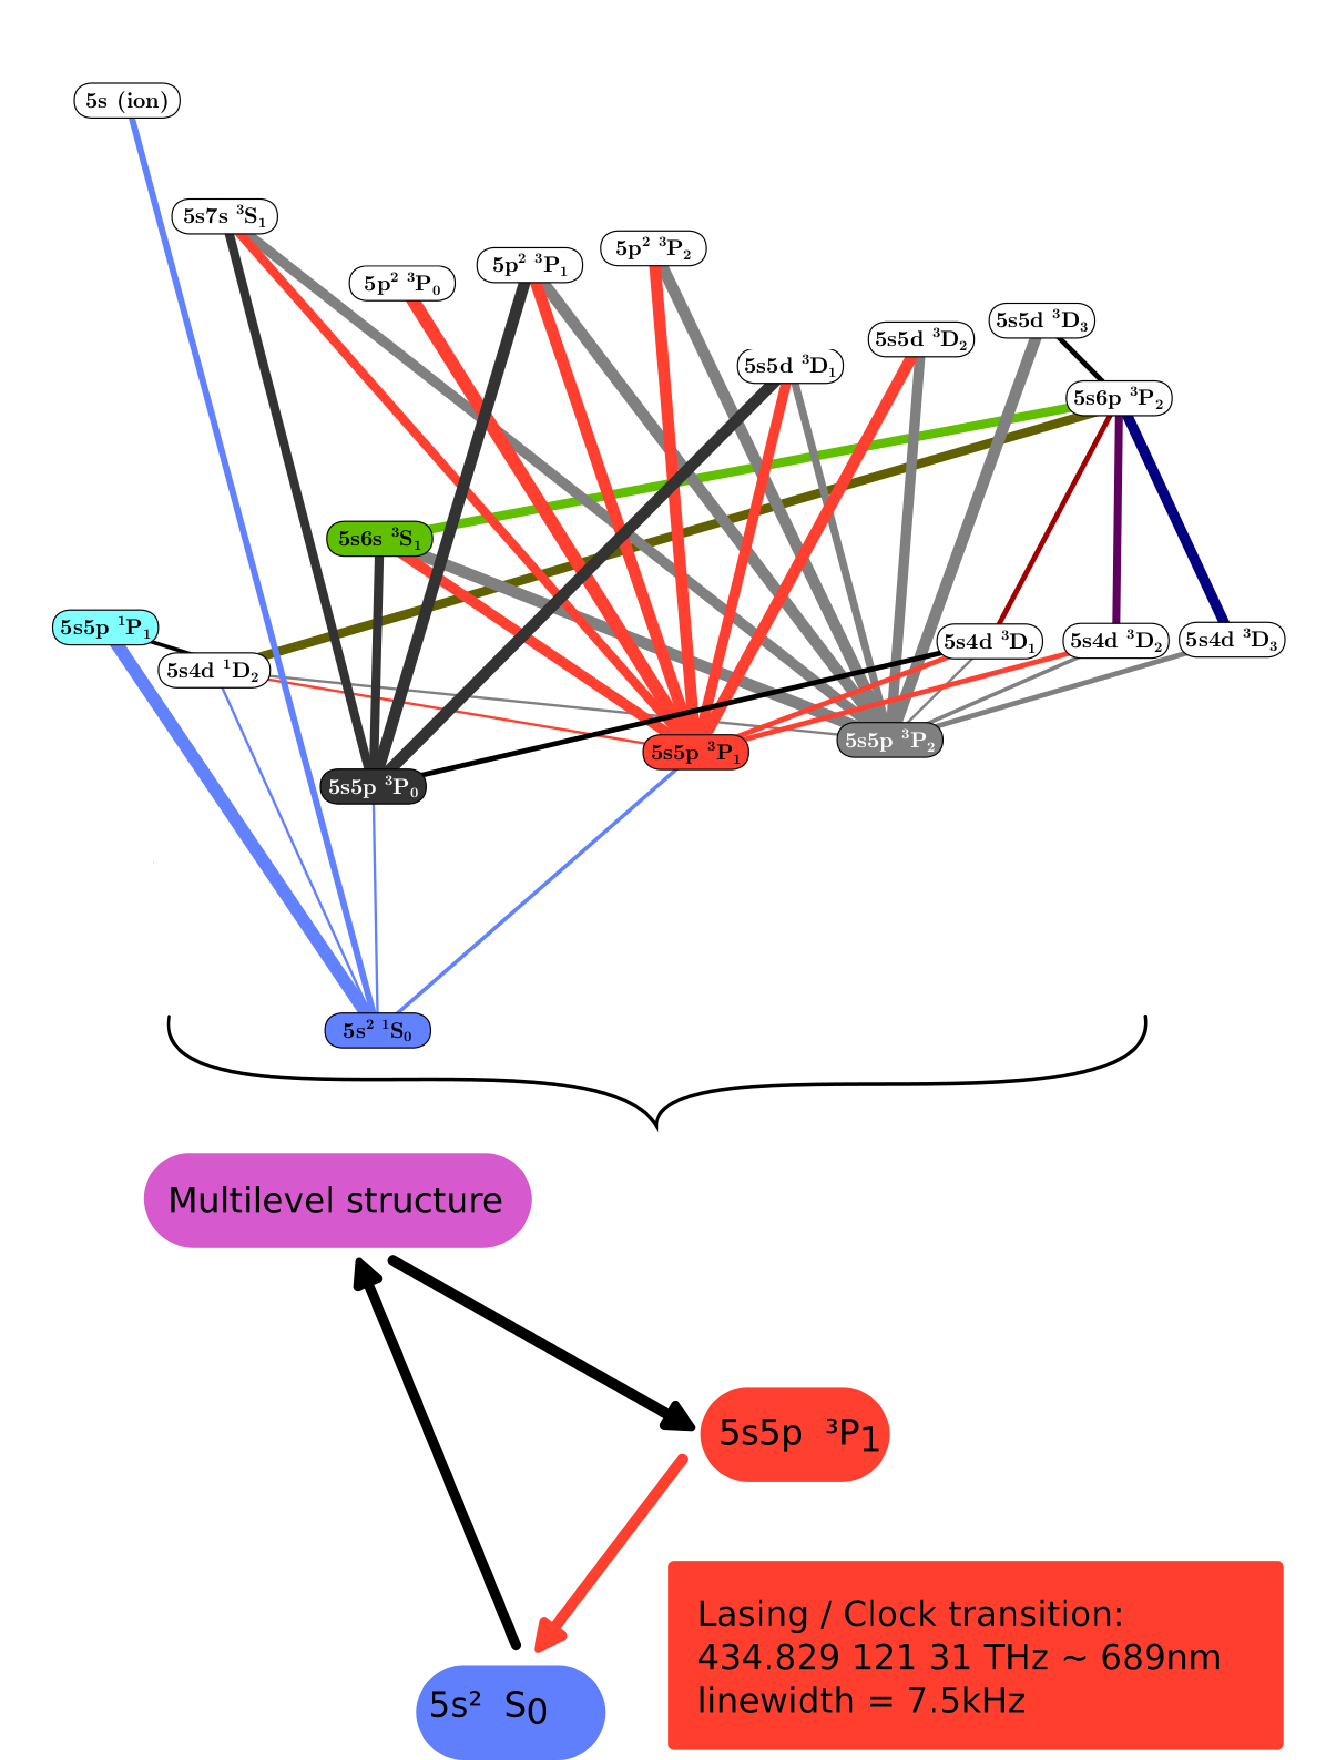
\includegraphics[width=\textwidth]{sr88}
\label{fig:sr88}
\end{figure}

In the quantum metrology group at the Niels Bohr institute, the atom used as the gain medium for this experiment is the strontium atom; more precisely, $^{88}$Sr. Among others, here are the main properties which led to this choice. $^{88}$Sr is the most abondant isotope of strontium at $\sim$82\% by mass. $^{88}$Sr has no nuclear spin, which gives it a simpler level structure compared to other isotopes and makes it easier to work with, especially for the many transitions involved in the repumping/cooling scheme. Strontium atoms have two electrons in their outermost shell, which gives them a structure of electronic transitions that is particularly useful in quantum metrology. The transition  $^1S_0$-$^3P_1$ of $^{88}$Sr has a linewidth of 7.5kHz. Note that the transition $^1S_0$-$^3P_0$ has a nearly null linewidth (if no magnetic field is present) but demands much more control from a technical point of view. Therefore, the transition $^1S_0$-$^3P_1$ is useful for exploring the physics of metrological systems and developing systems where simplicity is also important.

In figure \ref{fig:sr88}, the levels refer to the electrons in the outermost shell in the \textit{Russel-Saunders} notation $^{2S+1}L_J$ in addition of the standard electronical notation. Here $S$ is the total spin quantum number of the two electrons (as they are spin 1/2 particles, $S$ can be either 0 or 1). $L$ represents the orbital angular momentum quantum numbers by letters from spectroscopic notation ($S$ means 0, $P$ means 1 and $D$ means 2). $J$ denotes the total angular momentum quantum number from the spin-orbit coupling. The transition $^1S_0$-$^3P_1$ corresponds to the two-level structure modeled in the next chapter.



\chapter{Superradiance simulation}
\section{Optical Cavity}

We firstly introduce the \textit{optical cavity}. It consists of two mirrors mounted facing each other: the angle formed by one mirror and the optical axis is a right angle. The idea behind this simple setup is to select a discrete range of wavelengths defined by the space between the mirrors. 

Indeed, one can model the cavity as a one-dimensional box, then apply the wave equation $ \square \vv{E} = 0$ where $\square$ is the d'Alembertian operator and $\vv{E}$ the electric field's amplitude, together with the Maxwell equations $\nabla \cdot \vv{E} = \partial _x E = 0$. As the wave must vanish at the boundaries of the box (meaning that the energy cannot propagate outside of the box's region) one would find that the solutions are linear combinations of sinusoidal functions, each of them having a wavenumber multiple of $\frac{\pi}{L}$ where $L$ denotes the length of the box/cavity. We shall consider that our model is situated in a vacuum chamber, leading to the refractive index $n=1$ for the void and the well known constant $ c$ for the speed of light. Then, thanks to the relation $\omega = ck$ we see that the angular frequency is also quantized.\footnote{R.Loudon derives rigorous equations in sections 1.1 and 1.2 of \textit{Quantum Theory of Light}.} It is important to note that the argument is valid for other refractive indices and higher dimensions (i.e in 2D, 3D, ...).

With a more pragmatic point of view, one can think of this wavelength selection as an interferometer. In fact, let's imagine for a while that we emplace a cavity in front of the sun, fast enough to capture a beam of sunlight. Then we stop the clock before further propagation. Mathematically, the waves which are different from the selective frequency vansih instantaneously, because of the presence of the cavity. However, physically, the full spectrum of the sun still resides between the two mirrors. Then if we run the clock again, the light is reflected from the back mirror. As we captured a continous stream, the $\pi$-dephased reflected light encouters the incoming light: interference happens and after a couple of round-trips, only the waves generating an in-phase match at each round-trip (i.e with a space-frequency or wave-number $\frac{n\pi}{L}, n\in \llbracket 0, +\infty \llbracket $) remains by constructive interference, creating standing waves of the same frequency. On the other hand, all the other frequencies produce after reflection, on average over some round-trips, a destructive phase difference: the sum shall give a null coefficient in terms of amplitude for those given frequencies. Although this is a simple explanation, two things are important to note:
\begin{itemize}
  \item For the constructive interference case, we say that we need to be in-phase after one round-trip, meaning that after two reflections, which happens after hitting both back and front mirrors of the cavity, the wave must replicate the same amplitude at any position. However, the electric field is not static but moves in space. Then, it becomes more evident that twice the length of the cavity must be a multiple of the frequency in order to give the exact same phase.
  \item  For all the other frequencies, the phase difference is not random but actually well behaved. Nevertheless, After a couple of round-trips, the set of generated phase difference is unformly distributed among $ \left[ -\pi, \pi \right] $.
\end{itemize}

Thereby, that is why the device created by C.Fabry and A.Pérot in 1899 is called an \textit{interferometer} as, in their case, the light hit the mirrors with an angle, creating the famous pattern of fringes. Equivalently, this category of instrument is often named \textit{resonator} as the amplitude of the electric field is enhanced in the case of resonance with the cavity or decreases in other cases: by conception, it can be modeled as a classical harmonic oscillator or with the quantum equivalent.\footnote{As we will see later, each resonant frequency has a linewidth as a classical oscillator, in contrary to the quantum equivalent where the energy ladders (i.e the frequencies, in virtue of the relation $ \hbar \omega$) are well defined.}

In real experiments, the device is static and one prefers to let the light enter partially, to feed the cavity, and exit partially to collect the selected waves: only a part of the light is reflected into the cavity. In that way, we use \textit{partially reflective} mirrors parametrized by an electric field reflection coefficient $r$ and an electric field transmission coefficient $t$ obeying the relation $r^2 + t^2 = 1$ (the squared terms are the respective coefficient for the intensity of the field), meaning that all the absorbed energy must be re-emitted by the mirror, which is of course not fully true as some amount of the energy is scattered due to surface roughness. However, current manufacturers creates mirros with less than $0.01\%$ of loss and the above formula is sufficient for most of the applications.

One common approach to express the cavity response is the Airy distribution which represents the intensity ratio between the internal electric field and the \textit{launching} electric field (i.e the amount of \textit{feeding}-field succeding to transmit through the first mirror and penetrate the cavity), as a function of the phase accumulated for each round-trip\footnote{Of course, this is not the mathematical definition of the Airy distribution. However, we will see that this \textit{physical} distribution gives an actual Airy distribution.}:
\begin{equation}
\label{eqairy}
\textrm{Airy distribution} : A(\phi) = \frac{I_{circ}}{I_{launch}}(\phi)
\end{equation} 
In other words, it just makes the link between the enhancment factor of the cavity and the constructive-destructive interference phase pattern. In order to derive it, we shall use the circulating field approach \footnote{A. E. Siegman, section 11.3, \textit{Lasers}}:
\begin{itemize}
	\item A launching field: $ E_{launch} $
	\item A round-trip electric field which is the field after one complete round-trip: one reflection on the back mirror plus another on the front mirror. We call it $ E_{RT}$
	\item A circulating electric field which is the sum of the launched field and the round-trip one: $ E_{circ} =  E_{launch} + E_{RT}$. It is by definition the internal electric field after one rounde-trip (if we use an infinite sum instead, this would be the definition of the total electric field inside of the cavity).
\end{itemize}

Here, we use the phasor representation where the electric field (a real analytic signal) is split into two conjugate complex numbers:
\begin{align} 
\label{eq1}
E(x, t) &= \overline{E}(x, t) + \overline{E}^*(x, t) \quad \textrm{such that} \quad E(x, t) \in \mathbb{R}, \quad \overline{E}(x, t) \in \mathbb{C} \\\label{eq2}
&= 2 \Re \{  \overline{E}(x, t) \} 
\end{align}
Then, we consider fields evolving in time and in space along the optical axis $ x$. Moreover, one considers only the amplitude of the fields and deals with scalar equations. One can assume linearly polarized input field to get the same mathematical treament but the Airy distribution is valid for any kind of polarization and can be generalized for vectorial equations (i.e at higher dimension). Note that \eqref{eq1} is not a definition sign "$\stackrel{\text{def}}{=}$" as any analytic signal can be written in that form.\footnote{More explanations about the hypothesis and what an analytic signal implies in section ??}

Rewriting the equation for the circular field gives:
\begin{equation}
2\Re\{\overline{E}_{circ}\} = 2\Re\{\overline{E}_{launch}\} + 2\Re\{\overline{E}_{RT}\}
\end{equation}
which, by linearity and analyticity of the signal, is equivalent to:
\begin{equation}
\label{eqecirc}
\overline{E}_{circ} = \overline{E}_{launch} + \overline{E}_{RT}
\end{equation}

Now, one can express the round-trip field from the circular one, dephased by a certain angular amount. Indeed, one knows that each mirror add a phase of $\pi$ to the original field and the amplitude is modified by the reflection factor $r$. As a field of wave-number $k$ and propagating over a distance $l$ is shifted by:
\begin{equation}
ck \times \textrm{"propagation time"} = kl = \frac{\omega}{c}l
\end{equation} 
Then, after a complete round-trip, one obtains for the $E_{RT}$ a total angular shift of:
\begin{equation}
2\phi \stackrel{\text{def}}{=} \frac{2L}{c}\omega + 2\pi
\end{equation} 
where $\phi$ is the same phase as in \eqref{eqairy}. Thereby:
\begin{equation}
\label{eqrt}
\overline{E}_{RT} = r_1 r_2 e^{-i2\phi} \overline{E}_{circ}
\end{equation}
where $r_{1,2}$ are the reflection coefficients of the front and back mirror respectively. In other words, instead of propagating the field from its original value $ \overline{E}_{circ}$ through time or space to get a phase, we compute the relative phase $\phi$ from the length of the cavity $L$ with the field's frequency $\omega$.

One can highlight that for a characteristic space-frequency of the cavity $k=\frac{n\pi}{L}$, we have:
\begin{equation}
\label{phimodif}
2\phi = \frac{2L}{c} \times \frac{cn\pi}{L} + 2\pi = 2\pi(n + 1) \quad = \quad 0 \quad [2\pi]
\end{equation}
meaning that those frequencies generate constructive inteferences, thus, standing waves.

Putting \eqref{eqrt} in \eqref{eqecirc} leads to:
\begin{equation}
\frac{\overline{E}_{circ}}{\overline{E}_{launch}} = \frac{1}{1 - r_1 r_2 e^{-i2\phi}}
\end{equation}
Then, one uses the relation $ I \simeq \vert\overline{E}\vert^2$, which is valid for an average of the intensity over some periods of the $\overline{E}$-field \footnote{See section ??} and by the definition \eqref{eqairy}, one obtains:
\begin{equation}
\label{airyformula}
A(\phi) = \frac{1}{(1 - r_1 r_2)^2 + 4 r_1 r_2 \sin^2(\phi)}
\end{equation}
Moreover, to get the actual distribution that we observe through the cavity, that is to say, the enhancment factor at the output of the cavity, we set:
\begin{equation}
\label{airyformulasec}
A'(\phi) = (1-r_1^2)(1-r_2^2)\times A(\phi)
\end{equation}
where one uses the intensity transmission coeffcients $t_{1,2}^2 = 1-r_{1,2}^2$. Now, in order to sketch the function, independent of the size of the cavity $L$, we shall use the third term of the equality \eqref{phimodif} to reparametrize the round-trip dephasing variable $\phi$:
\begin{equation}
\label{phidef}
\phi = \pi(x+1) \quad = \quad \pi x \quad [\pi]
\end{equation}
where the integer variable $n$ has been replaced by the continuous one $x \in \mathbb{R}$ so that one can also investigate the behavior of the enhancment factor $A'(\phi) \sim A'(x)$ away from the resonant frequencies. Figure \ref{fig:airy-dist} is a normalized drawing\footnote{One divides the whole graph by $A'(0)$} of the airy distribution for a short amount of negative and positive resonant frequencies through a couple of reflexion coefficient $r_{1,2}$. 

\begin{figure}[h]
\caption{Normalized Airy distribution plot from -5 to 5 rads for three different sets of mirrors.}
\centering
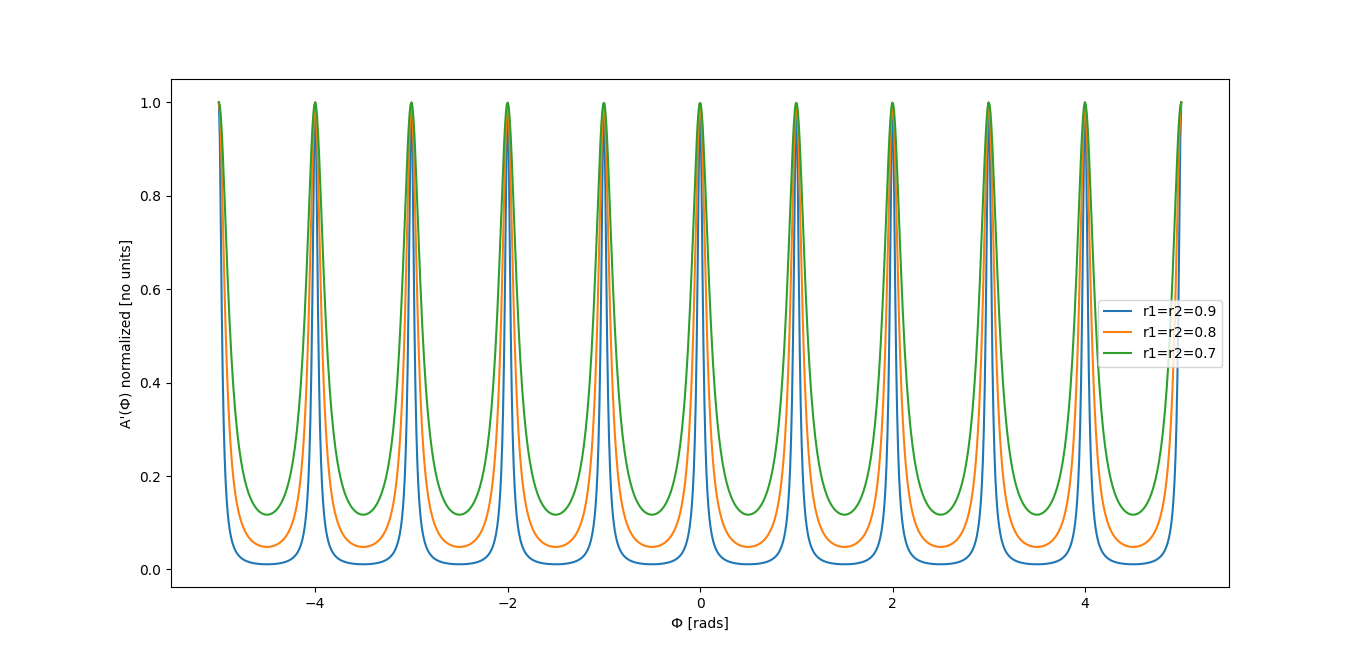
\includegraphics[width=\textwidth]{airy-dist}
\label{fig:airy-dist}
\end{figure}

To clarify, the abscisse coordinate is the factor quantity between two caracteristic frequencies $\frac{n\pi}{L}$, which can be equivalently spatial or temporal as we get ride of the constant $c$ in our calculation: then $x$ is a frequency divided by the free spectral range (FSR) In other words, for $x=\frac{1}{2}$, one gets the enhancment factor $A'$ for exactly a frequency halfway between two resonances, whereas $x=1$ gives the $A'$ factor for the first resonant frequency of the cavity.\footnote{One could say that the first resonant frequency is $x=0$ according to the figure or even the formula \eqref{airyformula} itslef. However, $x=0$ also means $n=0$: the launched field would have null frequency, which is not a physical solution.}

From those previous results, we can now define the \textit{full width at half maximum} (FWHM) which approximately represents how broad is the range around a resonant frequency where the field is modulated by more than one-half. Thanks to \eqref{airyformula}, one obtains $ A(0) / 2$ when the denominator respects:
\begin{equation}
(1 - r_1 r_2)^2 = 4 r_1 r_2 \sin^2(\Delta\phi) \Rightarrow \Delta\phi = \arcsin \left(\frac{1 - r_1 r_2}{2\sqrt{r_1r_2}} \right)
\end{equation}
with, in virtue of \eqref{phidef}:
\begin{equation}
\Delta\phi = \frac{\pi}{2}\Delta\nu
\end{equation}
where $\textrm{FWHM} \stackrel{\text{def}}{=} \Delta\nu$.

Finally, one can sketch the FWHM as a fonction of the mirror reflectivities $r_{1,2}$ and obtain figure \ref{fig:airy-fmwh}.

\begin{figure}[h]
\caption{FMWH (unit is frequency in rad/s) as function of the mirror reflectivities $r_{12} = r_1 = r_2$. As FSR is unity then the ordinate axis is the inverse of the finesse by definition.}
\centering
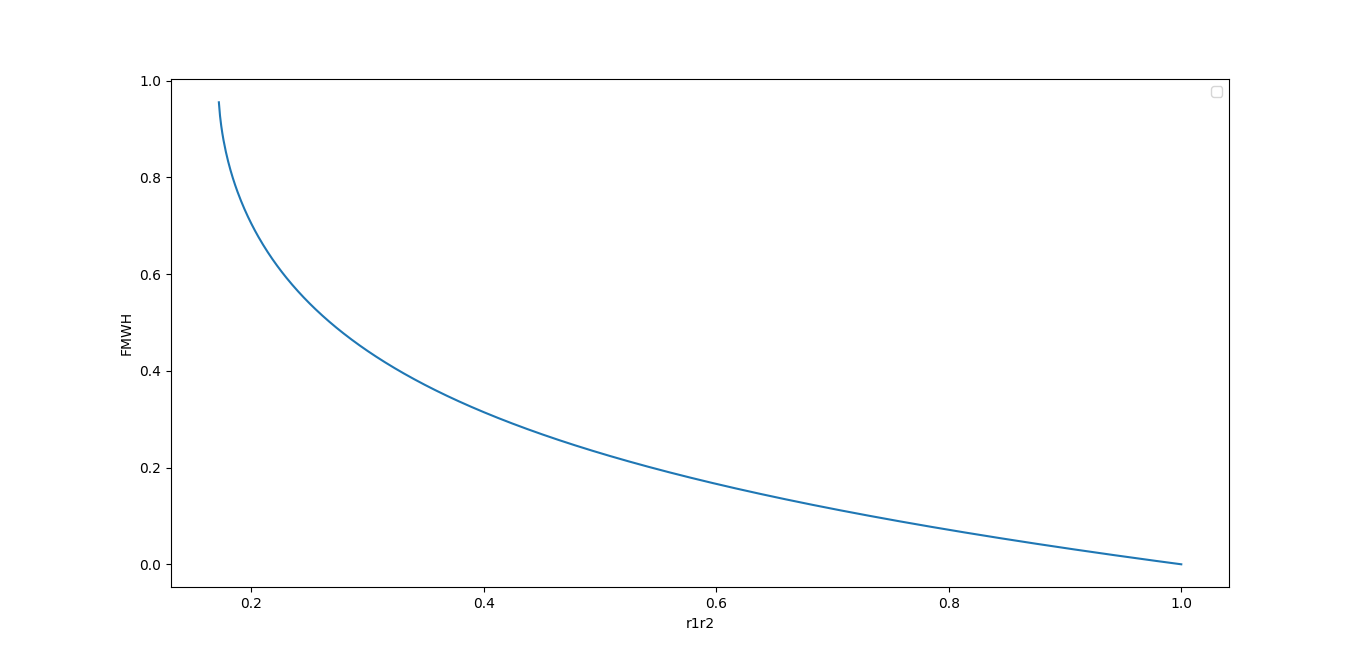
\includegraphics[width=\textwidth]{airy-fmwh}
\label{fig:airy-fmwh}
\end{figure}

Two important points are noticeable:
\begin{itemize}
	\item The linewidth of a cavity is invertly dependent on the mirrors reflectivity. In other words, larger is the transmission factor of the mirrors, the broader the frequency range around resonances, giving a \textit{less selective} cavity, and reciprocally. Then, two perfeclty reflective mirrors allow the FWHM to tend to zero: the cavity selects only and exactly the resonant frequencies $\frac{n\pi}{L}$. Formally, the \textit{selectivity} of a cavity is defined by its \textit{finesse} which reads $F \stackrel{\text{def}}{=} \frac{\textrm{FSR}}{\Delta\nu}$ where $FSR$ is the \textit{free spectral range}: one normalizes the distance (in term of frequency) separating two resonances by the linewidth.
	\item The function modeling the FWHM tends to infinity below a certain value which can be evaluated to approximately $r_1r_2 \approx 0.17$. That is due to the behavior of the $\arcsin$ which is not defined beyond $x=1$ for $x \in \mathbb{R}^+$. 
\end{itemize}

Nevertherless, it is always possible to build an experiment involving mirrors with high losses (i.e very low reflection or very high transmission). This is a limitation case of this \textit{Airy}-model and in the common scientific description of a cavity, one utilizes the Lorentzian approach where one defines a coherent time of the light from the reflection coefficient and the cavity length, then gets a differential rate equation of the amount of photons (i.e an exponential decay of the electric field) which, by virtue of the Fourier transform, gives a Lorentzian as a spectrum around one resonant frequency. Then, to obtain the full cavity spectrum, one has to sum each Lorentzian of all the resonances on the same graph.\footnote{Note that when treating the spontaneaous emission of an atom (or more formally, a two-level atomic system), one also deals with differential rate equations, which represents the exponential lifetime decay of the excitation, giving a Lorentzian as a spectrum: longer it takes to the system to decay, broader is the bandwidth. However, the analogy stops here: for a cavity, the whole electric field spectrum is affected by the linewidth, whereas, for a two-level atom, the spectrum represents the frequency uncertainty as the atom can spontaneously emit a photon with frequency slightly different from what the atom has been excited with.}

The Lorentzian model is highly faithfull to the real world experiment for all the possible reflective coefficients and tends to give the same caracteristic values (linewidth, finesse, ...) as the Airy-model from half to full reflective mirrors. However, it may seem to be less intuitive even if the derivation is straigthforward and, after all, the goal here was to show the principle of interference inside a cavity due to the round-trip dephasing term.

Finally, the next step for an optical cavity is, as many of physical systems, to interact with its environment. In other words, what happens if one adds an element, let's say atoms, inside of the cavity? This is basically the principle of lots of current experiments and advanced optical tools, namely the \textit{laser} among others, and the next section is decidated to the mathematical formulation of one first model for a cavity filled with a gain medium.

\section{Jaynes-Cummings model}

First of all, our system is composed of:
\begin{itemize}
	\item An electric field inside a cavity: this E-field is quantized and can only be a superposition of resonances.
	\item A single two-level system: this system has a structure of ground-excited state and can represent a transition of an atom for example.
\end{itemize}

When quantizing the E-field inside of a box of volume $V = L^3$ (i.e the cavity in three dimensions), one finds that the corresponding hamiltonian operator is [??Loudon p143]:
\begin{align}
\hat{H}_{cav} &= \int_{cavity} \left[\epsilon_0 \hat{E}(\vv{r}, t) \cdot \hat{E}(\vv{r}, t) + \mu_0^{-1} \hat{B}(\vv{r}, t) \cdot \hat{B}(\vv{r}, t)\right] \quad dV\\
&= \sum_{\vv{k}} \sum_{\lambda} \hbar \omega_{c,\vv{k}} \left( \hat{a}_{\lambda \vv{k}}^\dag \hat{a}_{\lambda \vv{k}} + \frac{1}{2} \right)
\end{align}
where $\hat{E}(\vv{r}, t)$ and $\hat{B}(\vv{r}, t)$ are respectively the electric and magnetic operators; $\epsilon_0$ and $\mu_0$ the electric and magnetic susceptibility of the vacuum respectively, $\omega_{c,\vv{k}}$ the frequency mode; $\lambda=\pm 1$ the polarization; $\hat{a}_{\lambda \vv{k}}^\dag$ with $\hat{a}_{\lambda \vv{k}}^\dag$ the ladders operator of the field.

Now, we define the electric field as exactly a unique mode with a unique polarization. Thereby:
\begin{equation}
\hat{H}_{cav} = \hbar \omega_c \left( \hat{a}^\dag \hat{a} + \frac{1}{2} \right)
\end{equation}
where we dropped the subscripts $\vv{k}$ and $\lambda$. In other words, we represent the electric wave as a perfectly coherent field which fits a resonance of the cavity at frequency $\omega_c$. As we can see, this one-mode cavity system is treated as a quantum harmonic oscillator.

Then comes the choice of the model for the ground-excited system. Sometimes, in the litterature [??MandelWolf], one utilizes another quantum harmonic oscillator with bosonic modes, namely:
\begin{equation}
\label{sec_bosonic_mw}
\hat{H}_{atom} = \hbar \omega_a \left( \hat{b}^\dag \hat{b} + \frac{1}{2} \right)
\end{equation}
where $\hat{b}$ is the bosonic operator of the two-level system. However, this model allows mutliple excited levels and the energy of the atom-system is artifically restrained to the first two levels.

In fact, an advantageous choice is to use the spin-half quantum system:
\begin{equation}
\hat{H}_{atom} = \hbar \omega_a \hat{\sigma_z}
\end{equation}
where $\hat{\sigma_z}$ is the third Pauli matrix.
This model allows us to use the spin-down $\ket{\downarrow}$ as the ground state with an energy: \begin{equation}
E_g \stackrel{\text{def}}{=} \bra{\downarrow}\hat{H}_{atom}\ket{\downarrow} = -\hbar\omega_a
\end{equation}
and $\ket{\uparrow}$ as the excited state with an energy:
\begin{equation}
E_e \stackrel{\text{def}}{=} \bra{\uparrow}\hat{H}_{atom}\ket{\uparrow} = \hbar\omega_a
\end{equation} Moreover, the Pauli matrices can exponentiates to the Lie algebra of SU(2) then follows similar commutator relations, namely:
\begin{equation}
\label{sigma_commut}
{\displaystyle [\hat{\sigma} _{j},\hat{\sigma} _{k}]=2i\varepsilon _{jkl}\,\hat{\sigma} _{l}}
\end{equation} 
where $\varepsilon _{jkl}$ is the Levi-Civita symbol. For the ladder operators $\hat{\sigma}_{\pm}=\hat{\sigma}_x \pm i\hat{\sigma}_y$, one can esasily prove the following projections:
\begin{equation}
\label{sigmapm_rules}
\hat{\sigma}_+ \ket{\downarrow} = \ket{\uparrow} \quad\quad
\hat{\sigma}_- \ket{\downarrow} = 0 \quad\quad
\hat{\sigma}_- \ket{\uparrow} = \ket{\downarrow} \quad\quad
\hat{\sigma}_+ \ket{\uparrow} = 0 \quad\quad
\end{equation}
which means that one can excite a ground state or damp an excited state but one cannot excite an already excited state or damp a ground state: the spin-1/2 model is restrained to a pair of states by definition.\footnote{From an autor to another, the eigenvalues may differ from a constant (in particular by a factor of $2$). Keep in mind that the Pauli matrix operators are taken from $\hat{\sigma}_i = \frac{2}{\hbar}\hat{S}_i$ where $\hat{S}_i$ is the spin operator.}

Now that we got the hamiltonian operators for the cavity field and the two-level system, we use the tensor product in order to create a quantum system all-encompassing those two systems:
\begin{equation}
\hat{H}_{JC} = \hat{H}_{atom} \otimes \mathbb{1}_{cav,2} + \mathbb{1}_{atom,n} \otimes \hat{H}_{cav} + \hat{H}_{int}
\end{equation}
where $\mathbb{1}_{cav,2}$ and $\mathbb{1}_{atom,n}$ are the identity operators for the Hilbert-space of the cavity and the atom respectively. Naturally, by their definition the Hilbert-space of the atom is of dimension $2$ (i.e two states form the basis) whereas the Hilbert-space of the cavity is of dimension $n$ as the quantum harmonic oscillator is associated to a Fock-space of the same dimension (i.e one has $n$ possible different levels of energy for the electric field). In other words, we build another Hilbert-space of dimension $2n$ from two separated system.\footnote{$\hat{H}_{atom}$ and $\hat{H}_{cav}$ are often refered to the energy of the atom and the cavity field respectively, which is a bit tendencious as this is only true when one takes those two systems separately, but falls down as soon as we mix them and add the interaction term: the eigenvalues (i.e energies) with an interaction are very different from the eigenvalues of the separated systems. Moreover, a hamiltonian operator corresponds to the energy if and only if it is \textit{explicitly} independent of time (which is the case here but it is always nice to precise the reason).} We also defined $\hat{H}_{int}$ as an additional hamiltonian operator belonging to an Hilbert-space which is of dimension $2n$ by construction: this new term arises from the physical interaction of the two systems but not by the \textit{mixture} of the cavity and atom systems (i.e there is nothing related with the tensor product). This interaction term can be mathematically formulated with the electric field's acting on the dipole constitued by the atom:
\begin{equation}
\hat{H}_{int}  \stackrel{\text{def}}{=} -\hat{d}\cdot\hat{E}(\vv{r}, t)
\end{equation}
where $\hat{d}$ is the dipole operator in term spin-half operators (using Pauli matrices) and $\hat{E}$ the quantized electric field of the cavity. After centering the frame on the atom with $\vv{r} = 0$, the interaction hamiltonian transforms as:
\begin{equation}
\hat{H}_{int} = \hbar g \left[ (\hat{\sigma}_+ - \hat{\sigma}_-) \otimes (\hat{a}^\dag - \hat{a})\right]
\end{equation}
where $g$ is the coupling constant arising from multiple constant terms belonging to the dipole and electric operators: $g$ defines \textit{how strong/often} the cavity field and the atom will exchange energy.
Finally, one obtains the complete hamiltonian operator for the Jaynes-Cummings model:
\begin{align}
\hat{H}_{JC} &\stackrel{\text{def}}{=} \hat{H}_0 + \hat{H}_{int}\\
&= \hbar \omega_c \left( \hat{a}^\dag \hat{a} + \frac{1}{2} \right) \otimes \mathbb{1}_{cav,2} + \mathbb{1}_{atom,n} \otimes \hbar \omega_a \hat{\sigma_z} + \hbar g \left[ (\hat{\sigma}_+ - \hat{\sigma}_-) \otimes (\hat{a}^\dag - \hat{a})\right]\\
\label{hjc_original_frame}
&= \hbar \omega_c \hat{a}^\dag \hat{a} + \hbar \omega_a \hat{\sigma_z} + \hbar g \left[ (\hat{\sigma}_+ - \hat{\sigma}_-) (\hat{a}^\dag - \hat{a})\right]
\end{align}
where we omit the tensor product on the last line and remove the $\frac{1}{2}\hbar\omega_c$, which is only a choice of reference for the vacuum energy (i.e here we set zero). In the future, the \textit{atomic} operators will lies on the right of the \textit{field} operators in order to remind the implicit tensorial structure of the system.\footnote{Note that we can reverse the tensor product order as long as one does not involve the coefficient of the states and this artifical sort is only present to clarify the notation and equations.}

Then, we shall change the reference frame of the hamiltonian in order to deal only with the frequency difference $\Delta\omega \stackrel{\text{def}}{=} \omega_c - \omega_a$, called \textit{detuning}. It will be advantageous for the simulation part and also allow us to apply a very common approximation. In this way, we use a U(1) symmetry for the JC-hamiltonian in this manner:
\begin{align}
\hat{H}_{JC} &\rightarrow U\hat{H}_{JC}U^{-1} + i\hbar\dot{U}U^{-1}\\
\ket{\psi} &\rightarrow U\ket{\psi}
\end{align}
where $\ket{\psi}$ is a solution of the Schrödinger equation for the JC-hamiltonian; $U$ is a unitary operator with its inverse $U^{-1}$ belonging to its dual space, involving $U^{-1}=U^{\dag}$; $\dot{U}$ is the one-time derivative of $U$. It can be proven that the transformed hamiltonian and $U\ket{\psi}$ vector plugged into the Schrödinger equation, give the same equation as the JC-hamiltonian and $\ket{\psi}$. Thereby, if one finds a solution $\ket{\phi}$ of the transformed system, then $U^{\dag}\ket{\phi}$ gives $\ket{\psi}$ which is a solution of the original system.

In our case, we choose the unitary transformation as:
\begin{equation}
\label{unitary_trans_def}
U \stackrel{\text{def}}{=} e^{\frac{i\omega_at}{\hbar}\hat{H}_0} = e^{i\omega_at(\hat{n} + \hat{\sigma}_z)}
\end{equation}
where we utilize the common photon number operator of the field, $\hat{n} = \hat{a}^{\dag}\hat{a}$. As the U(1) symmetry is essentially a rotation along the complex unitary circle, we explicitly choose here a rotation of $\omega_at$ which means that the transformed hamiltonian will be placed in the same frame as the atom: one calls this frame the \textit{rotating frame}.

One finally obtains the following parts for the transformed hamiltonian\footnote{See appendix \ref{unit_transfo}}
\begin{align}
i\hbar \dot{U} U^{\dag} &= -\hbar\omega_a(\hat{n} + \hat{\sigma}_z)\\
U\hbar \omega_c\hat{n} U^{\dag} &= \hbar\omega_c\hat{n}\\
U\hbar \omega_a\hat{\sigma}_z U^{\dag} &= \hbar\omega_a\hat{\sigma}_z\\
U\hbar g\hat{\sigma}_+\hat{a} U^{\dag} &= \hbar g\hat{\sigma}_+\hat{a}\\
U\hbar g\hat{\sigma}_-\hat{a}^{\dag} U^{\dag} &= \hbar g\hat{\sigma}_-\hat{a}^{\dag}\\
\label{rwa_1}
U\hbar g\hat{\sigma}_+\hat{a}^{\dag} U^{\dag} &= e^{2i\omega_at}\hbar g\hat{\sigma}_+\hat{a}^{\dag}\\
\label{rwa_2}
U\hbar g\hat{\sigma}_-\hat{a} U^{\dag} &= e^{-2i\omega_at}\hbar g\hat{\sigma}_-\hat{a}
\end{align}
As we shall us the detuning $\Delta\omega$ for the transformed hamiltonian instead of the respective cavity and atom frequency, it makes sense to write down a strong hypothesis on the system: $\omega_a \sim \omega_c$ which means that one assumes that the cavity and atom frequencies have the same order of magnitude. Thereby, the terms \eqref{rwa_1} and \eqref{rwa_2} are rotating extremely fast compared to our reference frame, about twice the cavity or atom frequency, and are qualified of \textit{anti-resonant}. Then, those terms average to zero over some cycles and can be discarded. This approximation is called the \textit{rotating wave approximation} (RWA).\footnote{Here, we firstly change the reference frame in order to introduce the RWA. However, this is not necessary. Indeed, the RWA only influence the interaction hamiltonian and one can apply this approximation directly in \eqref{hjc_original_frame} through the interaction picture evolution.}

At the end of the day, one finds the transformed hamiltonian:
\begin{equation}
\label{HJC}
\hat{H}_{JC} \rightarrow \hbar\Delta\omega\,\hat{n} + \hbar g \left(\hat{\sigma}_+ \hat{a} + \hat{\sigma}_- \hat{a}^{\dag} \right)
\end{equation}
that we rename by convenience and without ambiguity $\hat{H}_{JC}$. One may first notice that the atomic hamiltonian term vanished and only the field operator remains of $\hat{H}_0$: that is due to the new frame which \textit{follows} the atomic frequency, then the transformed $\hat{H}_{cav}$ is proportional to the detuning. It is also interesting to see how a \textit{generic} JC-state (i.e $\ket{\uparrow} \otimes \ket{n}$ or $\ket{\downarrow} \otimes \ket{n}$ which are also called \textit{bare states}) is influenced by the transformed interaction hamiltonian:
\begin{align}
\hat{H}_{int} \cdot \ket{\uparrow} \otimes \ket{n} &= \hbar g \left[ (\hat{\sigma}_+ \otimes \hat{a}) \cdot (\ket{\uparrow} \otimes \ket{n}) + (\hat{\sigma}_- \otimes \hat{a}^{\dag}) \cdot (\ket{\uparrow} \otimes \ket{n}) \right]\\
&= \hbar g \left[ \hat{\sigma}_+\ket{\uparrow} \otimes \hat{a} \ket{n} + \hat{\sigma}_- \ket{\uparrow} \otimes \hat{a}^{\dag} \ket{n} \right]\\
&= \hbar g \left[ 0 + \ket{\downarrow} \otimes \sqrt{n+1}\ket{n+1} \right]\\
&= \hbar g \ket{\downarrow} \otimes \sqrt{n+1}\ket{n+1} \stackrel{\text{def}}{=} \hbar g \sqrt{n+1} \ket{\downarrow, n+1}
\end{align}
where we used \eqref{sigmapm_rules}. Equivalently:
\begin{align}
\hat{H}_{int} \cdot \ket{\downarrow, n} &= \hbar g \left[ \hat{\sigma}_+ \hat{a} \ket{\downarrow, n} + \hat{\sigma}_- \hat{a}^{\dag} \ket{\downarrow, n} \right]\\
&= \hbar g \sqrt{n} \ket{\downarrow, n-1}
\end{align}
In other words, in the first case, an excited two-level system decays into its ground state, releasing a photon into the field (i.e the total energy is conserved), whereas in the second case, an atom \textit{at rest} absorbs a photon of the field and ends up in its excited state: this is intuitively how one may imagine the interaction between the atom and the cavity field system.

In order to solve the system evolution, one wants to diagonalize the hamiltonian by finding the eigenstates and the eigenvalues. It turns out that $\hat{H}_{JC}$ can be written by $2\times 2$ blocks in the JC-states:\footnote{The reason comes from the bare states being degenerated with eigenvalue $n+1$ when applied on the non-transformed base hamiltonian $\hat{H}_0$.}
\begin{equation}
\label{jc_block}
\hat{H}_{JC} = \bigotimes_n \begin{bmatrix}
\hbar \Delta\omega \, (n-1) & \hbar g \sqrt{n}\\
\hbar g \sqrt{n} & \hbar \Delta\omega \, n
\end{bmatrix}
\end{equation}
where $n$ under the tensor product is the fock space dimension associated to the cavity system.

After diagonalizing\footnote{See appendix \ref{eigen_vals_states}} each block of \eqref{jc_block}, one finds the following eigenvalues and eigenstates:
\begin{align}
\label{jc_eigens}
E_{n, \pm} &\stackrel{\text{def}}{=} \hbar\Delta\omega\,(n-\frac{1}{2}) \pm \hbar\sqrt{4g^2n + \Delta\omega ^2}\\
\ket{n, +} &\stackrel{\text{def}}{=} \cos\left(\frac{\theta_n}{2}\right) \ket{\uparrow, n - 1}  + \sin\left(\frac{\theta_n}{2}\right) \ket{\downarrow, n}\\
\ket{n, -} &\stackrel{\text{def}}{=} \cos\left(\frac{\theta_n}{2}\right) \ket{\downarrow, n}  - \cos\left(\frac{\theta_n}{2}\right) \ket{\uparrow, n - 1}
\end{align}
with:
\begin{equation}
\label{tan_theta_n}
\tan\left(\theta_n\right) = -\frac{2g\sqrt{n}}{\Delta\omega}
\end{equation}

To finish with the JC-model, we shall demonstrate one relevant case: the \textit{Rabi flopping} (or more explicitly the Rabi oscillations) when the detuning is null or can be assimilated as vanishing (i.e $\Delta\omega = 0$). Thereby, one starts with the two-level system as excited with an \textit{empty} cavity field:
\begin{equation}
\ket{\psi(0)} \stackrel{\text{def}}{=} \ket{\uparrow, n = 0} = \cos\left(\frac{\theta_{1}}{2}\right) \ket{1, +} - \sin\left(\frac{\theta_{1}}{2}\right) \ket{1, -}
\end{equation}
where we rewrite the initial state in terms of eigenstates.

Then, applying the spatial evolution operator, one finds\footnote{See appendix \ref{spatial_evol_op}}
\begin{align}
\ket{\psi(t)} &= e^{-\frac{i}{\hbar}\hat{H}_{JC}t}\\
&= \cos\left(\Omega t\right) \ket{\uparrow, 0} - i \sin\left(\Omega t\right) \ket{\downarrow, 1}
\end{align}
where we defined the Rabi frequency $\Omega = 2g$. Making the projection (i.e a measurement) along $\ket{\uparrow, 0}$ or $\ket{\downarrow, 1}$ and one ends up with the Rabi oscillations sketched on figure  \ref{fig:rabi-no-delta} where we set $g=1$:

\begin{figure}[h]
\caption{Rabi oscillations for the simple initial state $\ket{\uparrow, 0}$.}
\centering
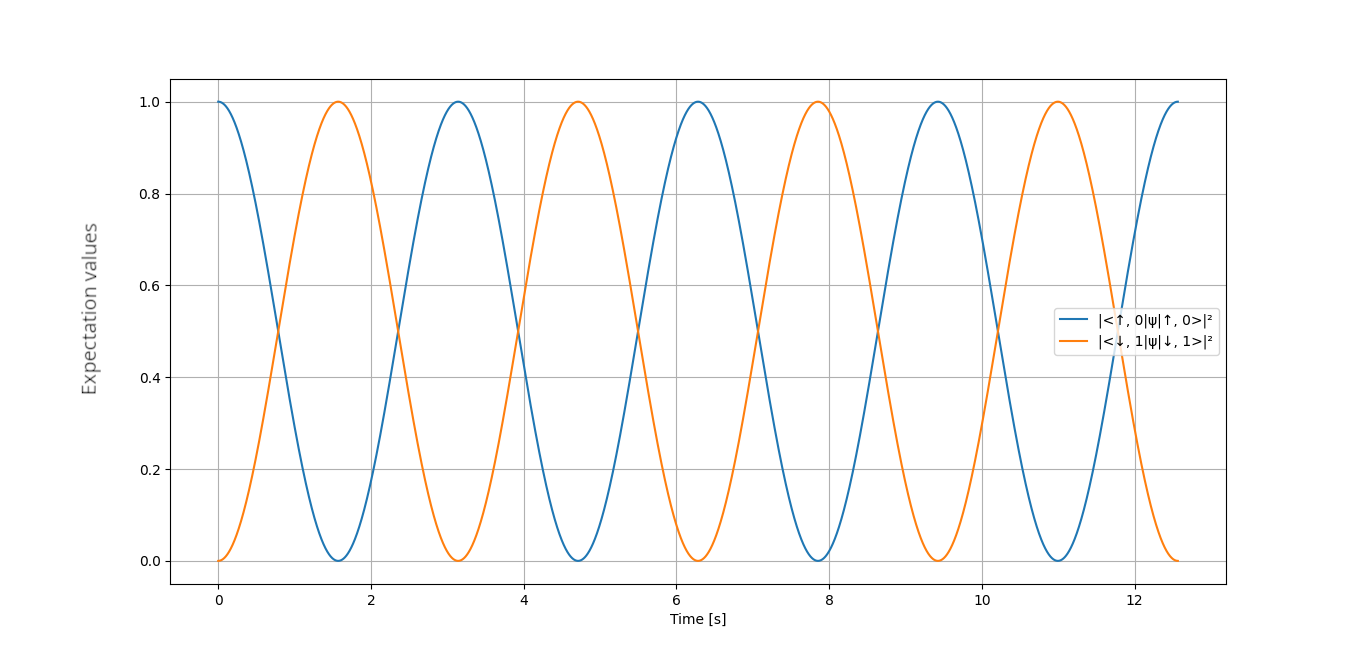
\includegraphics[width=\textwidth]{rabi-no-delta}
\label{fig:rabi-no-delta}
\end{figure}

As we can see on figure \ref{fig:rabi-no-delta}, the probabilities of finding one photon with the atom in its ground state, while no photon with the atom in the excited state, oscillate in opposite phase.

\begin{figure}[h!]
\caption{Rabi oscillations for the initial state $\ket{\uparrow, 0}$ with different detunings.}
\centering
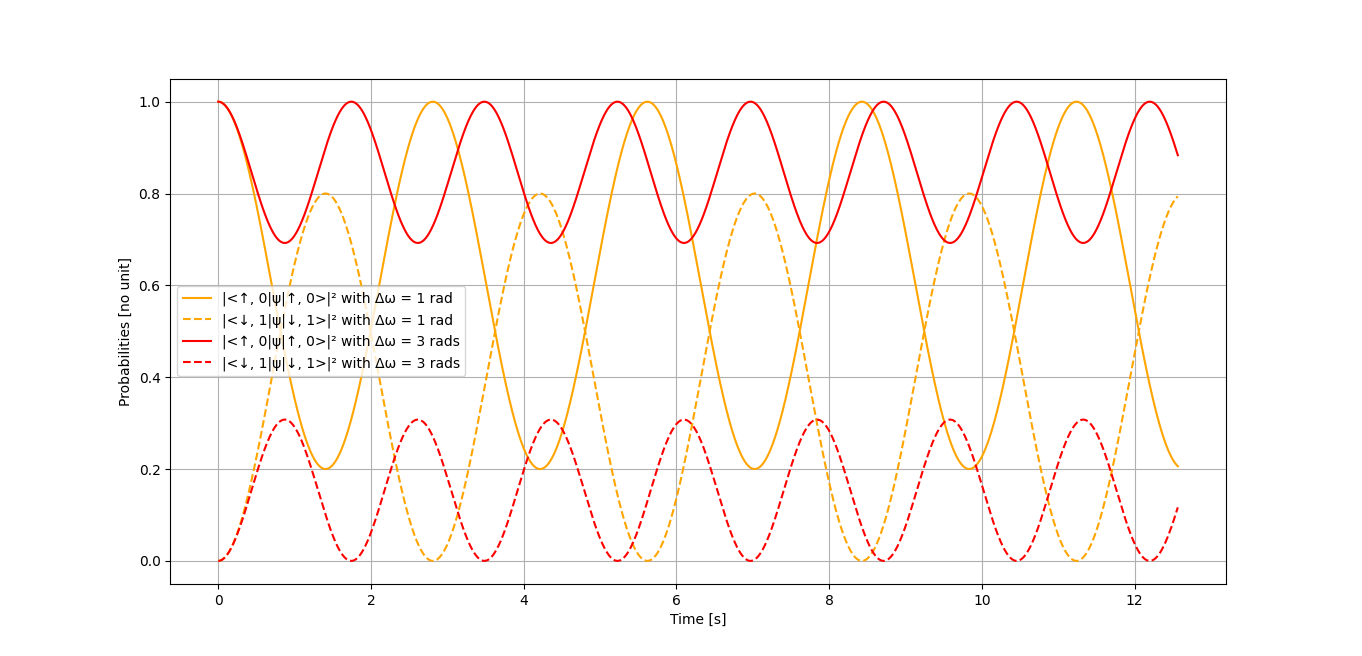
\includegraphics[width=\textwidth]{rabi-prog-delta}
\label{fig:rabi-prog-delta}
\end{figure}

Numerically, if one puts progressively a small detuning (i.e $\omega_a$ is still about the same order of magnitude of $\omega_c$), one can numerically sketch figure \ref{fig:rabi-prog-delta} where we see that the energy transfer is progressively discarded as we increase the detuning: the probabilities of inverting the intial state decreases.\footnote{Of course, it depends on the initial state. Here we chose to work with the pair $\ket{\uparrow, 0}$ and $\ket{\downarrow, 1}$ but similar behaviors happen for other states.} However, the \textit{rate}, at which the energy \textit{may} be transfered, increases: this behavior follows from \eqref{tan_theta_n}.

As we can notice, this model is mainly limited by its atomic level capability which is of number of two. Thereby, one would probably like to theoretically predict the behavior for many two-level systems (or equivalently several spins). Then, we shall introduce an extension of this model in the next section.

\section{Tavis-Cummings model}


In order to include more atoms, one needs to extend the Hilbert space involved into the JC-model. In fact, there are two ways of coupling more two-level systems, linked to the question: "Are the sub-systems distinguishable?". Indeed, here is the first \textit{naïve} idea to introduce $N$ atoms:
\begin{align}
\label{dist_sig_1}
\hat{\sigma}_i &\rightarrow \hat{\sigma}_i^1 \otimes \mathbb{1}^{2,...,N} + \mathbb{1}^{1} \otimes \hat{\sigma}_i^2 \otimes \mathbb{1}^{3,...,N} + ... + \mathbb{1}^{1,...,N-1} \otimes \hat{\sigma}_i^N\\
\label{dist_sig_2}
&\stackrel{\text{def}}{=} \sum_{j=1}^{N} \hat{\sigma}_i^j
\end{align}
where $i \in \left[x,y,z\right]$ and the upper indices indicate the Hilbert spaces involved into the operator owning them: $\mathbb{1}^{k,...,m}$ is the identity operator for the group of spaces from $k$ to $m$.\footnote{We intentionnaly split the tensor product in the transformation \eqref{dist_sig_1} for the sake of clarity even if the tensor product can be reversed. However, we drop the tensor notation in definition \eqref{dist_sig_2} for simplicity.}
As this transformation is made of linear combination of two-level system and as the unitary transformation in the previous section, involving commutator rules from the Pauli matrices, are still valid by independency of a system to another (i.e \eqref{sigma_commut} can be upper indexed for each Hilbert space), this leads to an equivalent hamiltonian of \eqref{HJC}:
\begin{equation}
\hbar\Delta\omega\,\hat{n} + \hbar g \sum_{j=1}^{N} \left(\hat{\sigma}_+^j \hat{a} + \hat{\sigma}_-^j \hat{a}^{\dag} \right)
\end{equation}
Thereby, this extended system is composed of $N+1$ independent sub-system with dimension scaling as $2^N \times N_{Fock}$ where $N_{Fock}$ is the space dimension of the cavity system. By \textit{independent}, we mean that each atom-like system is distinguishable from another. However, we do not have good reason to modelize our original experiment with independent atoms. Even worse, the superradiant effect is allowed by a collective ensemble, that is to say the atoms are indistinguishable and react as a whole multi-level system.\footnote{The second harmonic oscillator defined in \eqref{sec_bosonic_mw} could make sense but as the original argument in the JC-model, this bosonic structure doesn't allow a closed set of energies (i.e the atom group excitation could tend to infinity).} Indeed, R.H. Dicke, in its original paper [??] of coherent radiation process, states that the atom to atom distance (hence the gaz volume) must be much smaller than the wavelength of the surrounding electric field in order to reach an enhanced and coherent radiation. Nevertheless, in our experiment, the atomic cloud does not respect this condition for superradiance but as the atoms are enclosed into a cavity, this leads to collective interaction from the field to the cloud of atoms, hence indistinguishability.

Therefore, as the spins are assumed to be identical in \eqref{dist_sig_2}, one uses instead the collective spin operator:
\begin{equation}
\label{sig_change_s}
\sum_{i=1}^{N} \hat{\sigma}_j^i \rightarrow \frac{2}{\hbar} \hat{S}_j
\end{equation}
where $\hat{S}_j$ follows the spin algebra similar to the Pauli matrices with, among other relations, the commutator:
\begin{equation}
{\displaystyle [\hat{S} _{j},\hat{S} _{k}]=i\hbar\varepsilon _{jkl}\,\hat{S} _{l}}
\end{equation}
The change of variable \eqref{sig_change_s} allows to write, in the case of spin-$1/2$, $\hat{\sigma}_j = \frac{2}{\hbar}\hat{S}_j$ Then, one obtains the following hamiltoninan for indistinguishable N two-level systems:
\begin{equation}
H_{TC} \stackrel{\text{def}}{=} \hbar\Delta\omega\,\hat{n} + g \left(\hat{S}_+ \hat{a} + \hat{S}_-\hat{a}^{\dag} \right)
\end{equation}
where the constant $g$ \textit{swallows} a factor of 2 (i.e $2g \rightarrow g$). Historically, this type of hamiltonian refers to the Tavis-Cummings (TC) model as it only includes a co-rotating term by the RWA (which is the actual interaction part of the TC-hamiltonian) then the TC-model keep the U(1) symmetry. However, R.H. Dicke proposes another hamiltonian involving a counter-rotating term of $\hat{S}_- \hat{a} + \hat{S}_+\hat{a}^{\dag}$ (without unitary transformation) which breaks the U(1) symmetry: we shall not utilize the Dicke model here because a posteriori (by simulation), the additional term is unnecessary.

This model may represent a group of N atom where each atom can be in its ground state or excited state, interacting with a radiation field. For practical reason, this system of two-level system is often called a \textit{gain medium} as models involving such systems can be utilized for LASER simulation where the the lasing beam is enhanced by population inversion.

By construction, if one choose a unique atom with $N=1$, the spin structure is quantized as:
\begin{equation}
s = \frac{1}{2} \quad; \quad m = \pm \frac{1}{2}
\end{equation}
which allows two pure states, similar to $\ket{\uparrow}$ and $\ket{\downarrow}$. Morevover, if one increases the number of atom to $N=2$, one get three pure states:
\begin{align*}
s = 1 \,;\, m = -1 \quad &\sim \quad \ket{\downarrow, \downarrow}\\
s = 1 \,;\, m = 1 \quad &\sim \quad \ket{\uparrow, \uparrow}\\
s = 1 \,;\, m = 0 \quad &\sim \quad \ket{\downarrow, \uparrow} \quad \textrm{or} \quad \ket{\uparrow, \downarrow}\\
\end{align*}
where the last case involves two well different states of the two distinguishable systems. However, our atoms are represented as a collective spin structure which means that they are indistinguishable leading to considerate those two different states as identical from an energy point of view. In that way, our system of collective spin system scales as $2 \times \frac{N}{2} + 1 = N + 1$ for $N$ two-level systems and the global system involving the field scales now as $(N+1) \times N_{Fock}$ which looses the exponential behavior from the distinguishable case: this is a great advantage from a simulation point of view.

In other words, one can create a global excitation state $\ket{s = N/2, m = N/2}$ where all the atoms are excited and, at the opposite, a global ground state $\ket{s = N/2, m = -N/2}$. However, for other values of $m$, one cannot \textit{say} or predict which atom or sub-group of atoms are excited: this leads to degeneracies determined by the binomial coefficient,
\begin{equation}
\textrm{Number of "equivalent state"} = \frac{N!}{N_{excited}!(N-N_{excited}!)} = \begin{pmatrix}
N\\
N_{excited}
\end{pmatrix} 	
\end{equation}
where $N_{excited}$ is the number of excited two-level syste, and the \textit{equivalent} term holds for a collective spin system point of view. It is well known that the maximum of the binomial coefficient is reached for $N_{excited} = \frac{N}{2}$ meaning that the maximum amount of degeneracies is reached when the gain medium is half-populated of excited entities.

Finally, we obtained a hamiltonian which looks very close to the JC-model and the natural question which now arises is: "How does one populate the gain medium of excitation? How the photons may leak oustside of the cavity?". For the first case, one may start with a state of the desired excited population. However, it exists another approach where our quantum system is included into a quantum \textit{bath}, allowing energy to leak in and out.\footnote{We do not go further into the spectrum caracterisation of $\hat{H}_{TC}$, even if it may be done, because the master equation shall complexify the exact solution at a point that we use another approach for the numerical simulation.}

\section{Open quantum systems and the master equation}

Firstly, we introduce the density operator in order to also treat probabilistic mixtures:
\begin{equation}
\label{def_dens_mat}
\rho \stackrel{\text{def}}{=} \sum_i p_i \ket{\psi_i}\bra{\psi_i}
\end{equation}
where $\left\lbrace \ket{\psi}, p_i \right\rbrace$ is a set of pure state associated to a probability. Equivalently, if we fix an arbitrary basis $\left\lbrace \ket{i} \right\rbrace$ of the Hilbert space, we can write:
\begin{equation}
\label{deftwo_dens_mat}
\rho = \sum_{i,j} \rho_{i,j} \ket{i}\bra{j}
\end{equation}
where $\rho_{i,j}$ are the matrix coefficient of $\rho$ in the the given basis. It can be shown that a density matrix fulfill three essential conditions which are equivalent in regard of \eqref{def_dens_mat}:
\begin{itemize}
	\item $\rho$ is positive semi-definite: $\bra{v} \rho \ket{v} \geqslant 0, \quad \forall \ket{v}$
	\item $\rho$ is hermitian: $\rho = \rho^\dagger$
	\item $\rho$ is trace one: $\sum_i p_i = \sum_i \rho_{i, i} = 1$
\end{itemize}

As a ket state obeys to Schrodinger's equation, one can derive a similar equation of evolution for a density matrix, called \textit{Liouville - von Neumann} equation. Indeed, one may consider the two following equations:
\begin{equation}
i\hbar\partial _t\ket{\phi} = \hat{H}\ket{\phi} \Leftrightarrow -i\hbar\partial _t\bra{\phi} = \bra{\phi}\hat{H}
\end{equation}
where $\ket{\phi}$ is any solution to the Schrodinger equation. Then coupling those to \eqref{def_dens_mat} one shall find:
\begin{equation}
\label{vonneuman}
i\hbar\dot{\rho} = \left[ \hat{H}, \rho \right] \Leftrightarrow \dot{\rho} = -\frac{i}{\hbar} \left[ \hat{H}, \rho \right]
\end{equation}
where we define $\dot{\rho} \stackrel{\text{def}}{=} \partial _t \rho$.One can notice that this equation relies on the Schrodinger point of view, where the states evolves in time whereas the operators are static. At the opposite, the Heinsenberg picture gives:
\begin{equation}
\dot{\hat{X}} = \frac{i}{\hbar} \left[ \hat{H}, \hat{X} \right]
\end{equation}
where $\hat{X}$ is any operator without explicit time dependence (i.e $\partial _t \hat{X} = 0$).\footnote{This brutal change of picture shall be crucial for the section introducing $g^1$ and $g^2$ simulation with the cumulant expansion technique.}

At this point, we are able to simulate the evolution of the closed quantum TC-model for any initial state. It turns out that our experiment involves several \textit{leaks} (in and out) in term of global energy: they are three in number:
\begin{itemize}
	\item Cavity leak: as mentionned in section 1.1, the cavity purpose is to release a part of the electric field (at the cost of the linewidth broadened) in order to actually collect the radiation. In other words, some photons are transmitted through one of the mirror: this is a global energy loss in our TC system.
	\item Gain medium leak: counter-intuitively, the atoms (or dipole systems) may incoherently release a photon with frequency very different to the actual cavity resonances. Those photons does not couple to the surrounding electric field and are lost: this effect is another global energy loss and is called \textit{spontaneous decay into free space}.
	\item Gain medium repump: as the expriments works on a \textit{quasi}-continous radiation, even starting with excited atoms (which is not the case), we need to add some energy in order to compensate the phase coherent decay of our atoms which produce the actual radiation (through the cavity leak). This is a global energy gain in the system.
\end{itemize}

Therefore, we introduce a quantum \textit{bath} system which represent the environment of our TC quantum system. The total hamiltonian reads\footnote{For simplicity, we drop the tensor product but it is important to keep in mind that the total hamiltonian lives into an Hilbert space with higher dimension than the TC system.}
\begin{equation}
\hat{H}_{total} = \hat{H}_{TC} + \hat{H}_{bath} + \hat{H}_{TC-bath}
\end{equation}
Then, one chooses the interaction picture where the evolution is set by the interaction hamiltonian $\hat{H}_{TC-bath}$ between the bath and our system. One starts with a bath and our system without cross correlation. Afterward, the time evolution of the density matrix of the total system can be written in term of an infinite iterative equation: one uses the \textit{Born} approximation stating that the bath-TC interaction coupling is weak compared to the size of the bath, allowing to \textit{cut} the inifinte serie as the bath evolution is independent of the system evolution. Then, one makes a last assomption that the bath has a \textit{short memory} meaning that the correlations are not significant for long time intervals if the bath is subject to fast dynamics: this is the \textit{Markov} approximation.

At the end of the day, one obtains the open quantum system equation, often called the \textit{master equation}:
\begin{equation}
\dot{\rho} = -\frac{i}{\hbar} \left[ \hat{H}, \rho \right] + \sum_j \gamma_j \left( \hat{L}_j \rho \hat{L}_j^\dagger - \frac{1}{2} \left\lbrace \hat{L}_j^\dagger \hat{L}_j, \rho \right\rbrace \right)
\end{equation}
where $j$ indexes the different \textit{leak} operators $\hat{L}_j$, often called \textit{jump} operators or more simply \textit{lindblad} operators. Also, $\gamma_j$ are the associated \textit{damping} rate (even if the operator's purpose may be to add energy) and the curly brackets are the anti-commutator relation.
Equivalently for the Heisenberg picture, we find:
\begin{equation}
\label{master_eq_heis}
\dot{\hat{X}} = \frac{i}{\hbar} \left[ \hat{H}, \hat{X} \right] + \sum_j \gamma_j \left( \hat{L}_j^\dagger \hat{X} \hat{L}_j - \frac{1}{2} \left\lbrace \hat{L}_j^\dagger \hat{L}_j, \hat{X} \right\rbrace \right)
\end{equation}
where one may notice the sign difference in front of the commutator and the opposite dagger symbol on the lindblad operator of the first term of the sum.
In our case, we get three lindblad operators, representing the various \textit{leaks} of the TC quantum system:
\begin{itemize}
	\item The cavity leak or \textit{cavity decay} operates at a rate $\kappa$. The associated lindblad operator is the destruction operator of the cavity field $\hat{a}$: this ladder operator removes energy from the harmonic oscillator.
	\item The spontaneous decay into free space operates at a rate $\gamma$. The associated lindblad operator is the collective spin ladder operator $\hat{S}_-$ which \textit{collectively} removes energy from the atomic system.
	\item The repump operates at a rate $\nu$ and is associated to the lindblad operator $\hat{S}_+$: we assume that an external laser \textit{feeds} collectively the ensemble of two-level system, which has for effect to add energy into the TC quantum system.
\end{itemize}

To summarize, the density matrix evolution responds to the following first order differential equation:
\begin{align}
\label{rho_master_eq}
\begin{split}
\dot{\rho} = &\left[ \rho \, , \, i\Delta\omega\,\hat{n} + \frac{i}{\hbar} g \left(\hat{S}_+ \hat{a} + \hat{S}_-\hat{a}^{\dag} \right)\right]\\
&+ \kappa \left( \hat{a}^\dagger \rho \hat{a} - \frac{1}{2} \left\lbrace \hat{a}^\dagger \hat{a}, \rho \right\rbrace \right)\\
&+ \gamma \left( \hat{S}_- \rho \hat{S}_+ - \frac{1}{2} \left\lbrace \hat{S}_+ \hat{S}_-, \rho \right\rbrace \right)\\
&+ \nu \left( \hat{S}_+ \rho \hat{S}_- - \frac{1}{2} \left\lbrace \hat{S}_- \hat{S}_+, \rho \right\rbrace \right)
\end{split}
\end{align}
where with have taken $\hat{H}_{TC}$ as the hamiltonian. There is a similar equation (close to a sign and dagger operators) for any operator $\hat{X}$. This differential equation is a system of linear differential equation in a sense that each time derivated term of the density matrix is dependent of linear terms of the density matrix. In other words:
\begin{equation}
\dot{\rho_{i,j}} = \sum_{k,l} \alpha_{k,l}^{i,j} \rho_{k,l}
\end{equation}
where $\rho_{i,j}$ are the density matrix components with indices $(i,j)$ $\alpha_{k,l}^{i,j}$ are fixed complex coefficent dependent on operator values and constants. 

Thereby, this system is numerically solvable with standard integration methods as the Runge-Kutta approach.\footnote{Note that the Runge-Kutta method is not restricted to linear systems as, by definition, this approach treats any function $f$ where $\dot{y} = f(y, t)$ and $y$ can be any variable of any vector space: $y \in \mathbb{R}, \mathbb{R}^2, \mathbb{R}^3, ..., \mathbb{C}, \mathbb{C}^2, \mathbb{C}^3, ...$ for examples.} As one could think, if the system is linear, it should be diagonalizable hence exactly solvable by exponentiation. However, this approach is not possible in the form of \eqref{rho_master_eq} as the equation is treating the density operator as, obsviously, a matrix. 

Nevertheless, one may introduce a new concept called the \textit{linearization} of the density operator. In fact, the density matrix lies in the Hilbert space $\mathscr{H}_{TC} = \mathscr{H}_{cav} \otimes \mathscr{H}_{atoms}$ and one may transform this matrix into a vector lying in the new space $\mathscr{H}_{TC} \otimes \mathscr{H}_{TC}$, which is often called the \textit{Fock-Liouville space}. In this way, \eqref{deftwo_dens_mat} becomes:
\begin{equation}
\rho = \sum_{i,j} \rho_{i,j} \ket{i}\bra{j} \rightarrow \sum_{i,j} \rho_{i,j} \ket{i} \otimes \ket{j} = \begin{pmatrix}
\rho_{0,0}\\
\rho_{0,1}\\
\vdots\\
\rho_{n-1,n-1}
\end{pmatrix}
\stackrel{\text{def}}{=} \kket{\rho}
\end{equation}
where $n$ is the dimension of $\mathscr{H}_{TC}$. Then, the von-Neumann equation \eqref{vonneuman} transforms as:
\begin{equation}
\dot{\rho} = -\frac{i}{\hbar}\left( \hat{H}\rho - \rho\hat{H} \right) \rightarrow \kket{\dot{\rho}} = -\frac{i}{\hbar} \mathcal{H}\kket{\rho}
\end{equation}
where $\mathcal{H}$ is a superoperator defined as $\mathcal{H}\kket{\cdot} \rightarrow \left[ \hat{H}, \cdot \right]$.\footnote{This is not a definition symbol because the left side does not lie in the same space as the right side: $\mathcal{H}$ belongs to the \textit{superspace} $\mathscr{H}_{TC} \otimes \mathscr{H}_{TC}$ whereas the commutator lies in $\mathscr{H}_{TC}$ only.} Similarly, one may define the lindblad superoperator:
\begin{equation}
\mathcal{D}[\hat{L}_j] \kket{\rho} \rightarrow \hat{L}_j \rho \hat{L}_j^\dagger - \frac{1}{2} \left\lbrace \hat{L}_j^\dagger \hat{L}_j, \rho \right\rbrace
\end{equation}
and the master equation becomes:
\begin{align}
\begin{split}
\kket{\dot{\rho}} &= -\frac{i}{\hbar} \mathcal{H}\kket{\rho} + \kappa \mathcal{D}[\hat{a}] \kket{\rho} + \gamma \mathcal{D}[\hat{S}_-] \kket{\rho} + \nu \mathcal{D}[\hat{S}_+] \kket{\rho}\\
&= \left(-\frac{i}{\hbar} \mathcal{H} + \kappa \mathcal{D}[\hat{a}] + \gamma \mathcal{D}[\hat{S}_-] + \nu \mathcal{D}[\hat{S}_+]\right)\kket{\rho} \\
&= \mathcal{L}\kket{\rho}
\end{split}
\end{align}
where we defined the Liouvillian superoperator $\mathcal{L}$ from the second line of the equation. From that, it is possible to calculate the eigenvalues and eigenvectors in order to find the exact values of $\kket{\rho}$ at any time $t$.\footnote{Note that as the Liouvillian superoperator is not hermitian by construction, the right and left eigenvectors are associated to different eigenvalues. See [??] for more details.}

However, the first limitation of this method is the size of the system. Indeed, as $\mathscr{H}_{TC}$ scales according to $(N+1) \times N_{Fock}$ then the Fock-Liouville space scales as the square:
\begin{equation}
\textrm{dim}\left(\mathscr{H}_{TC} \otimes \mathscr{H}_{TC}\right) = \left((N+1) \times N_{Fock}\right)^2
\end{equation}
In order to hold the decay of the atoms, the Fock space associated to the cavity field must be at least the same dimension as the number of two-level systems.\footnote{In practice, we take twice the size for \textit{security} and a double check of the photon number, after computation, asserts that we are not overflowing the Fock space.} Then, for $N$ dipoles as a gain medium:
\begin{equation}
\textrm{dim}\left(\mathscr{H}_{TC} \otimes \mathscr{H}_{TC}\right) \sim N^4
\end{equation}
Thereby, the number of components for the vector $\kket{\rho}$ scales according to the same rule. Moreover, the number of components inside the \textit{super}-matrix representing the Liouville superoperator scales as the square of it, namely as $N^8$. For instance, let's say that we want to numerically simulate our model with one hundred atoms: the super-matrix owns $10^{16}$ components. As each component is a complex number represented by two floats of 32-bit each (in the low precision case): 8 byte per component. At the end of the day, we need approximately $80,000$ TB only to store the Liouvilian superoperator\footnote{1TB = 1000 GB which is somehow a common hard-drive capacity for the family computers on the current tech-market (2024).}. Ideally, we would like to simulate a couple of millions of atoms.

Unfortunately, the first method of solving, involving the RK intergation, suffers the same problem for many particles: as we stay in the original Hilbert space $\mathscr{H}_{TC}$, the power scale is less important but many atoms simulation is still unreachable for more than a few hundreds of atoms. Even worse, this solution is not exact, in a sense that we get the solution for a finite time interval where the computation time is dependent on it!

This case is a good example of the classical computer limitation and this sort of problem is part of the reason of building a quantum computer/simulator. Indeed, one could make use of the parallelism behavior of the qubit in order to simulate many cross interaction at the same time. However, those kind of projects are not yet achieved and we have to find a \textit{smart} solution, in a sense that we are ready to lose a bit of precision in exchange of computation power and memory space. In fact, all the crossed terms essentially represent the multiple interaction holded by each atom. Secondly, the question we have to ask is: "what mesure do we want from the simulation?". As we shall see in later section, our interested correlation function are, roughly, the expectation values of operators accross the time. In other words, we absolutely do not care about the behavior of individual terms. So, what happens if one plugs directly the excpectation value on the "Heisenberg version" of the master equation \eqref{master_eq_heis}? This is the subject of the next section.

\section{Cumulant expansion method}

Firstly, even if we go into more details in chapter ?? about their signification, we have to recall what are the first and second order correlation function in term of quantum operators in order to visualize which sort of values we need to extract from the master equation.

Thereby, in the case of a non-stationary electric field, one can define the first order correlation function as:
\begin{equation}
\label{g1_classic_def}
{\displaystyle g ^{1}(t_{1},t_{2})\stackrel{\text{def}}{=}{\frac {\left\langle E^{*}(t_{1})E(t_{2})\right\rangle }{\sqrt{\left\langle \left|E(t_{1})\right|^{2}\right\rangle \left\langle \left|E(t_{2})\right|^{2}\right\rangle }}}}
\end{equation}
where $E(t) \in \mathbb{C}$ is the phasor representation of the electric field and the mean symbol $\left\langle \cdot \right\rangle$ is an ensemble average over a set of electric signal. Note that we also make the assumption that the correlation measurement is done at $r_1 = r_2 = 0$ for both detectors of the electric field.

In turns out that any eletric field can be quantized  with the help of an artificial \textit{quantization box} of volume $V$ and the associated formulas are:
\begin{equation}
{\displaystyle {\hat {E}}^{+}=i\sum \limits _{\vv {k} ,\lambda }{\sqrt {\frac {\hbar \omega _{k}}{2\epsilon _{0}V}}}{\hat {a}}_{\vv {k} ,\lambda }e^{i\vv {k} .\vv {r} }\vv {e} _{\vv {k} ,\lambda }} \quad \quad {\displaystyle {\hat {E}}^{-}=-i\sum \limits _{\vv {k} ,\lambda }{\sqrt {\frac {\hbar \omega _{k}}{2\epsilon _{0}V}}}{\hat {a}}^\dagger_{\vv {k} ,\lambda }e^{-i\vv {k} .\vv {r} }\vv {e}^* _{\vv {k} ,\lambda }}
\end{equation}
where ${\displaystyle \omega _{k}}$ is the mode frequency associated to the polarization vector ${\displaystyle \vv {k} }$, 
${\displaystyle \vv {e} _{\vv {k} ,\lambda }} \in \mathbb{C}^3$ is the unit vector perpendicular to 
${\displaystyle \vv {k} }$, with 
${\displaystyle \lambda }$ signifying one of the two vectors that are perpendicular to the polarization vector. Now, making the assumption that the electric field is composed of one frequency (i.e a unique mode of the \textit{fake}-cavity) and replacing the electric field phasor components by their quantum operator counterparts, one finds the quantum equivalent of the first order correlation function:
\begin{equation}
g^1(t_1, t_2) = \frac{\left\langle \hat{a}^\dagger(t_1)\hat{a}(t_2) \right\rangle}{\sqrt{\left\langle \hat{a}^\dagger(t_1)\hat{a}(t_1) \right\rangle \left\langle \hat{a}^\dagger(t_2)\hat{a}(t_2) \right\rangle}}
\end{equation}
where we may notice that the denominator terms are function of the mean photon number $\hat{n}$ at time $t_1$ and $t_2$. Moreover, we considered the time evolution of the electric field as the time evolution of the operators, in other words, the Heisenberg picture. This consideration comes from the fact that the numerator is a mean value of two operators evaluated at a different time each. Indeed, we define the mean value of any operator $\hat{X}$ as the quantum measurement of $\hat{X}$ over a pure state $\ket{\psi}$ or a density matrix $\rho$:\footnote{Equation \eqref{quantum_meas} is directly derivated from the second postulate (\textit{measurement postulate}) of the Quantum Mechanic Theory.}
\begin{equation}
\label{quantum_meas}
\left\langle \hat{X} \right\rangle_{\psi \, or \, \rho} = \bra{\psi}\hat{X}\ket{\psi} \quad or \quad \Tr \left[ \rho \hat{X} \right]
\end{equation}
Which leads, for the time evolution of the mean value, to the two famous pictures (considering a density matrix as the measured state):
\begin{align}
\begin{split}
\textrm{Schrödinger picture:} \quad\quad \left\langle \hat{X} \right\rangle_{\rho} (t) = \Tr \left[ \rho(t)\cdot \hat{X} \right]\\
\textrm{Heisenberg picture:} \quad\quad \left\langle \hat{X} \right\rangle_{\rho} (t) = \Tr \left[ \rho\cdot \hat{X}(t) \right]\\
\end{split}
\end{align}
If we set $\hat{X}(t_1,t_2) = \hat{Y}(t_1)\hat{Z}(t_2)$, it becomes obvious that the Heinsberg picture is appropriate:
\begin{equation}
\left\langle \hat{X} \right\rangle _{\rho} (t_1, t_2) = \Tr \left[ \rho \cdot \hat{Y}(t_1) \cdot \hat{Z}(t_2)\right]
\end{equation} 
In other words, we are looking for the time evolution of $\hat{a}^\dagger$ and $\hat{a}$ but not the time evolution of the initial state. By the way, those previous equations shows that the quantum $g^1$ is dependent on the choice of the initial state.

It is important to note that $g^1$ is by definition a 2D map\footnote{Only in its non-stationary form.}. As we are going to run numerical simulations through it, we can consider $t_2$ as a fixed value and compute the time evolution of $g^1$ according to $t_1$:
\begin{equation}
\label{quantum_g1_1D_map}
g^1(t_1)_{t_2} = \frac{\left\langle \hat{a}^\dagger(t_1)\hat{a}_{t_2} \right\rangle}{\sqrt{\left\langle \hat{n}(t_1) \right\rangle \left\langle \hat{n}_{t_2} \right\rangle}}
\end{equation}
which is a 1D map (i.e a function), then repeat the process for every $t_2$ of the targeted time interval.

Moreover, in the stationary case, the distribution of the the electric signal is independent of time and one may find that $g^1$ is only dependent on the time difference $t_1 - t_2 \stackrel{\text{def}}{=} \tau$:
\begin{equation}
g^1(\tau)_{stationary} = \frac{\left\langle \hat{a}^\dagger(t_2 + \tau)\hat{a}(t_2) \right\rangle}{\sqrt{\left\langle \hat{n}(t_2 + \tau) \right\rangle \left\langle \hat{n}(t_2) \right\rangle}}=\frac{\left\langle \hat{a}^\dagger(\tau)\hat{a}(0) \right\rangle}{\sqrt{\left\langle \hat{n}(\tau) \right\rangle \left\langle \hat{n}(0) \right\rangle}}
\end{equation}
where we set $t_2 = 0$ as the process is considered as stationary, hence, independent on the reference time. Note the similarities with the non-stationary case \eqref{quantum_g1_1D_map} from a computational point of view: the reference time $t_2$ is just a question of initial value of the operators $\hat{a}$ and $\hat{n}$.

Similarly, for the classical second order correlation fonction, one defines:
\begin{equation}
{\displaystyle g ^{2}(t_{1},t_{2})\stackrel{\text{def}}{=}{\frac {\left\langle E^{*}(t_{2})E^{*}(t_{1})E(t_{1})E(t_{2})\right\rangle }{\left\langle \left|E(t_{1})\right|^{2}\right\rangle \left\langle \left|E(t_{2})\right|^{2}\right\rangle}}}
\end{equation}
Then, the quantum equivalent reads as:
\begin{equation}
{\displaystyle g ^{2}(t_1, t_2)={\frac {\left\langle \hat{a}^\dagger(t_2)\hat{a}^\dagger(t_1)\hat{a}(t_1)\hat{a}(t_2)\right\rangle }{\left\langle \hat{n}(t_1) \right\rangle \left\langle \hat{n}(t_2) \right\rangle}}}
\end{equation}
As before, the stationary assumption allows us to write\footnote{It is possible to define $t_2 - t_1 \stackrel{\text{def}}{=} \tau$. This time reverse step does not affect the function itself as $g^2(\tau) = g^2(-\tau)$ for a stationary process. The same property hold for $g^1$.}:
\begin{equation}
{\displaystyle g ^{2}(\tau)={\frac {\left\langle \hat{a}^\dagger(0)\hat{a}^\dagger(\tau)\hat{a}(\tau)\hat{a}(0)\right\rangle }{\left\langle \hat{n}(\tau) \right\rangle \left\langle \hat{n}(0) \right\rangle}}}
\end{equation}

At the end of day, the desired quantities are complex values dependent on operator evolution. That is to say, we actually want the quantum measurement of the ladder and photon number operators. Then, let's start with the value $\left\langle\hat{a}^\dagger\right\rangle$ from the differential equation:
\begin{align}
\label{dtad_rough}
\begin{split}
\frac{d}{dt}\hat{a}^\dagger = &\quad\frac{i}{\hbar}\left[ \hat{H}_{TC}\, , \, \hat{a}^\dagger \right]\\
&+ \kappa \left( \hat{a}^\dagger \hat{a}^\dagger \hat{a} - \frac{1}{2} \hat{a}^\dagger \hat{a} \hat{a}^\dagger - \frac{1}{2} \hat{a}^\dagger \hat{a}^\dagger \hat{a} \right)\\
&+ \gamma \left( \hat{S}_+ \hat{a}^\dagger \hat{S}_- - \frac{1}{2} \hat{S}_+ \hat{S}_- \hat{a}^\dagger - \frac{1}{2} \hat{a}^\dagger \hat{S}_+ \hat{S}_- \right)\\
&+ \nu \left( \hat{S}_- \hat{a}^\dagger \hat{S}_+ - \frac{1}{2} \hat{S}_- \hat{S}_+ \hat{a}^\dagger - \frac{1}{2} \hat{a}^\dagger \hat{S}_- \hat{S}_+ \right)
\end{split}
\end{align}
which is the \textit{Heisenberg} equivalent of \eqref{rho_master_eq}.\footnote{We intentionally omit the artificial order of the operators that we made earlier for the implicit representation of the tensor structure: no ordering allows us to highlight the lindblad operators.} One uses the standard commutation relations, remembering that the collective spin operator does not lie into the same space as the cavity ladder operators then one obtains\footnote{See appendix \ref{cumu_exp_for_ad}}:
\begin{equation}
\label{ad_pure}
\frac{d}{dt}\hat{a}^\dagger = \left(i\Delta\omega - \frac{\kappa}{2} \right) \hat{a}^\dagger + \frac{ig}{\hbar} \hat{S}_+
\end{equation}
Making measurement according to a state $\rho$ and knowing that a projection is a linear operation on a time derivative, one gets:
\begin{equation}
\label{ad_mean_field}
\frac{d}{dt}\left\langle\hat{a}^\dagger\right\rangle = \left(i\Delta\omega - \frac{\kappa}{2} \right) \left\langle\hat{a}^\dagger\right\rangle + \frac{ig}{\hbar} \left\langle\hat{S}_+\right\rangle
\end{equation}
which is again a differential equation involving only complex (or real) numbers: we have lost all the cross interaction information contained inside the operator and reduced it to the mean value of the operators. However, this first order differential equation is of two variable instead of one as the master equation with the variable $\rho$. Indeed, $\left\langle\hat{S}_+\right\rangle$ is also time dependent and one needs its time evolution in order to solve the equation: in fact, we are actually treating a system of equations and are now looking for the second member. Then, we can reengage the process with the operator $\hat{S}_+$ instead and the differential equation is this time:
\begin{equation}
\frac{d}{dt}\left\langle\hat{S}_+\right\rangle = -2ig\left\langle\hat{S}_+ \hat{a}^\dagger\right\rangle + \hbar (\nu - \gamma)\left\langle \hat{S}_z \hat{S}_+\right\rangle - \nu \hbar ^2 \left\langle\hat{S}_+\right\rangle
\end{equation}
Unfortunately, this new equation leads to new variables, namely: $\left\langle\hat{S}_+ \hat{a}^\dagger\right\rangle$ and $\left\langle \hat{S}_z \hat{S}_+\right\rangle$. Moreover, the mean value or cross-correlation between two operators (or even for two random variable from a classical point of view) is not equal to the multiplication of the individual correlations: 
\begin{equation}
\left\langle \hat{X}\hat{Y} \right\rangle \neq \left\langle \hat{X} \right\rangle \left\langle \hat{Y} \right\rangle
\end{equation} 
Therefore, it makes sense to write:
\begin{equation}
\left\langle \hat{X}\hat{Y} \right\rangle = \left\langle \hat{X} \right\rangle \left\langle \hat{Y} \right\rangle
\end{equation} 
only if we assume that $\hat{X}$ and $\hat{Y}$ are independent in term of probability representation. In that case, one loses all the quantum interaction happening in the correlated variables: this approximation is named \textit{mean field approximation}.

If one applies this approximation, one shall obtain:
\begin{equation}
\label{sp_mean_field}
\frac{d}{dt}\left\langle\hat{S}_+\right\rangle = -2ig\left\langle\hat{S}_+ \right\rangle\left\langle\hat{a}^\dagger\right\rangle + \hbar (\nu - \gamma)\left\langle \hat{S}_z \right\rangle\left\langle\hat{S}_+\right\rangle - \nu \hbar ^2 \left\langle\hat{S}_+\right\rangle
\end{equation}
Now the only missing variable equation evolution is $\left\langle \hat{S}_z \right\rangle$. Then we repeat the process again and we find two more equations.
\begin{equation}
\label{sz_mean_field}
\frac{d}{dt}\left\langle\hat{S}_z\right\rangle = -ig\left\langle\hat{S}_+ \right\rangle\left\langle\hat{a}\right\rangle + ig\left\langle\hat{S}_- \right\rangle\left\langle\hat{a}^\dagger\right\rangle + \hbar (\gamma - \nu)\left\langle \hat{S}_- \right\rangle\left\langle\hat{S}_+\right\rangle - 2\nu \hbar ^2 \left\langle\hat{S}_z\right\rangle
\end{equation}
One can be tented to develop two more variables which would be $\left\langle\hat{S}_- \right\rangle$ and $\left\langle\hat{a}\right\rangle$. However, those two operators are the conjugate transpose of $\hat{S}_+$ and $\hat{a}^\dagger$ respectively and their quantum measurement is just complex conjugate:
\begin{equation}
\left\langle\hat{S}_- \right\rangle = \left\langle\hat{S}_+ \right\rangle^* \quad\quad \left\langle\hat{a}\right\rangle = \left\langle\hat{a}^\dagger\right\rangle^*
\end{equation}
Therefore, the three differential equations \eqref{ad_mean_field}, \eqref{sp_mean_field} and \eqref{sz_mean_field} form a complete system of equation, hence, can be solved taking the initial values as:
\begin{equation}
\left\langle \hat{a}^\dagger \right\rangle (t=0) = \Tr\left[ \rho \hat{a}^\dagger_0 \right]
\end{equation}
where $\rho$ is the initial density matrix of the system and $\hat{a}^\dagger_0$ is the common constructor operator\footnote{Note that a $t=0$, quantum measurements according to the Schrödinger or Heisenberg picture are equivalent.}. One may say that this system of equation is a \textit{closed} form in a sense that, with the mean field approximation, if one chooses any of the five operators $\hat{a}^\dagger$,$\hat{a}$, $\hat{S}_+$, $\hat{S}_-$ or $\hat{S}_z$ at the start, then the final set of differential would be exactly the same as \eqref{ad_mean_field}, \eqref{sp_mean_field} and \eqref{sz_mean_field} (taking into account the complex conjugated equations).

Now, we have to remember that, in addition of retrieving the quantum correlation lost with the mean field approximation (i.e a first order approximation), our goal is to get the evolution of correlation functions involving several operators. In fact, it is clear that if we develop a differential equation with $\left\langle\hat{S}_+ \hat{a}^\dagger\right\rangle$ for example, we shall get correlation variables involving three or more operators. Repeating the process will certainly give an infinity amount of differential equations. In other words, we have to \textit{break the loop} with a certain order of approximation. In this way, one may invoke the definition of the \textit{joint cumulant}:
\begin{equation}
\left\langle\hat{X}_1\hat{X}_2...\hat{X}_n\right\rangle_c \stackrel{\text{def}}{=} \sum_{p \in P(\mathcal{I})} (\vert p \vert - 1)!(-1)^{\vert p \vert -1} \prod_{B \in p} \left\langle \prod_{i \in B}\hat{X}_i\right\rangle
\end{equation}
where $\mathcal{I} = \left\rbrace 1,2, ..., n \right\rbrace$, $P(\mathcal{I})$ is the set of all partition of $\mathcal{I}$, $\vert p \vert$ is the length of the partition and B is successively each element of the partition. It is possible to prove (ref ??) that the joint cumulant is null if any operator $\hat{X}_i$ is independent of all the others (in term of probabilities). Then, the main approximation is to assume that, at a certain number of operator $m$ inside the cumulant, at least one of the operator among them is independent of the others. This implies $\left\langle\hat{X}_1\hat{X}_2...\hat{X}_m\right\rangle_c = 0$ and one may write:
\begin{equation}
\left\langle\hat{X}_1\hat{X}_2...\hat{X}_m\right\rangle = \sum_{p \in P(\mathcal{I})/\mathcal{I}} (\vert p \vert - 1)!(-1)^{\vert p \vert -1} \prod_{B \in p} \left\langle \prod_{i \in B}\hat{X}_i\right\rangle
\end{equation}
where $\mathcal{I} = \left\lbrace 1,2, ..., n \right\rbrace$ and $P(\mathcal{I})/\mathcal{I}$ is the set of all the partitions of $\mathcal{I}$ without $\mathcal{I}$ itslef. From that, it is obvious that the mean field approximation is condidering  this formula  with $m=2$. Then, for $m=3$:
\begin{equation}
\left\langle\hat{X}_1\hat{X}_2\hat{X}_3\right\rangle = \left\langle\hat{X}_1\hat{X}_2\right\rangle\left\langle\hat{X}_3\right\rangle + \left\langle\hat{X}_1\hat{X}_3\right\rangle\left\langle\hat{X}_2\right\rangle + \left\langle\hat{X}_2\hat{X}_3\right\rangle\left\langle\hat{X}_1\right\rangle - 2\left\langle\hat{X}_1\right\rangle\left\langle\hat{X}_2\right\rangle\left\langle\hat{X}_3\right\rangle
\end{equation}
and so on for $m>3$. This approximation is named the \textit{cumulant expansion method}.

At the end of day, the algorithmic approach is choosing an order $m$ where, if one finds a correlation variable with $m$ or more operators inside of the correlation brackets when developing the set of equations, one applies the cumulant expansion in order to transform a correlation variable of $m$ operators into several correlation variables of $m-1$ operators. In other words, $m$ is the amount of operators where one \textit{breaks the loop}. Finally, one may choose any order of approximation knowing that greater is the order (i.e, more operator we have inside the correlation brackets), more quantum correlations one takes into account (i.e more precision in the simulation) \textit{but} more equations one has to treat and more computational power is needed. The question is then to find a good compromise.

Nevertheless, at any order of the expansion one can go, the time evolution of the correlation variable involve the time evolution of all the operators inside of it at the same time reference. That is to say:
\begin{equation}
\left\langle\hat{X}_1\hat{X}_2\right\rangle (t) = \left\langle\hat{X}_1(t)\hat{X}_2(t)\right\rangle
\end{equation}
for instance. In other words, one cannot access the $g^1$ and $g^2$ values directly from this method as those two correlation invlove different time evolution of the operators. However, one may see from \eqref{quantum_g1_1D_map} that the desired differential equation needed for $g^1$ before making the quantum measurment (i.e before applying $\left\langle \cdot \right\rangle$) reads:
\begin{equation}
\frac{d}{dt_1} \left(\hat{a}^\dagger(t_1)\hat{a}_{t_2}\right) = \frac{d}{dt_1} \left(\hat{a}^\dagger(t_1)\right)\hat{a}_{t_2}
\end{equation}
where $\hat{a}_{t_2}$ is treated as a constant compared to $t_1$. We can see that the right term of the previous equation calls the already derivated formula \eqref{ad_pure} of $\hat{a}^\dagger$, which is of the form:
\begin{equation}
\frac{d}{dt_1} \hat{a}^\dagger(t_1) = f(\hat{a}^\dagger(t_1)) 
\end{equation}
where $f$ is basically the heisenberg version of the master equation. Then multiplying by a tme constant operator (compared to $t_1$), namely $\hat{a}_{t_2}$ \footnote{We make this choice of $\hat{a}_{t_2}$ in order to fit the $g^1$ notation but it is important to keep in mind that it could be any constant operator.}, one obtains:
\begin{equation}
\frac{d}{dt_1} \left(\hat{a}^\dagger(t_1)\right) \hat{a}_{t_2} = f(\hat{a}^\dagger(t_1)) \hat{a}_{t_2}
\end{equation}
which, in the case of \eqref{ad_pure}, reads as:
\begin{equation}
\frac{d}{dt_1}\left(\hat{a}^\dagger(t_1)\right)\hat{a}_{t_2} = \left(i\Delta\omega - \frac{\kappa}{2} \right) \hat{a}^\dagger(t_1)\hat{a}_{t_2} + \frac{ig}{\hbar} \hat{S}_+(t_1)\hat{a}_{t_2}
\end{equation}
Now, one can make a quantum measurement and gets:
\begin{equation}
\label{g1_explicit_cumu}
\frac{d}{dt_1}\left\langle\hat{a}^\dagger(t_1)\hat{a}_{t_2}\right\rangle = \left(i\Delta\omega - \frac{\kappa}{2} \right) \left\langle\hat{a}^\dagger(t_1)\hat{a}_{t_2}\right\rangle + \frac{ig}{\hbar} \left\langle\hat{S}_+(t_1)\hat{a}_{t_2}\right\rangle
\end{equation}
Of course, this \textit{multiplication followed by quantum measurement} must be applied to the whole set of differential equation in order to \textit{update} all the correlation variables: before obtaining \eqref{g1_explicit_cumu}, one derived the closed system of equation containing $\left\langle\hat{S}_+(t_1)\right\rangle$ but not $\left\langle\hat{S}_+(t_1)\hat{a}_{t_2}\right\rangle$\footnote{Algorithmically speaking, the set is first derived without applying the brackets (i.e quantum measurement), then the multiplication and brackets are applied.}.

The initial value of \eqref{g1_explicit_cumu} is expressed as:
\begin{equation}
\left\langle\hat{a}^\dagger(t_1)\hat{a}_{t_2}\right\rangle (t_1=0) = \left\langle\hat{a}^\dagger_0\hat{a}_{t_2}\right\rangle
\end{equation}
However, we do not dispose to this information as we only know the initial operator values $\hat{a}^\dagger_0$ and $\hat{a}_0$ but not the time evolution of $\hat{a}_{t_2}$. Nevertheless, if we derive a set of equation to a certain order allowing the access to the correlation variable $\left\langle\hat{a}^\dagger(t)\hat{a}(t)\right\rangle$, then we can get any intial value of \eqref{g1_explicit_cumu} for $t_1=t_2$: solving the system of differential equation leads to solution with $t_1\geqslant t_2$ which represents the lower-half of the 2D map accoring to the diagonal $t_1=t_2$ as on Fig ??.

This initial value problem only stands for non-stationary processes. Indeed, for a stationary process, we firstly have to numerically compute a time interval long enough to reach the steady-state of the correlation variables. Then, as stated in the begining of this section, $g^1$ for a stationary process is dependent on the time difference $\tau$, that is to say, once $\left\langle\hat{a}^\dagger(t)\hat{a}(t)\right\rangle$ is stable after a certain amount of time, let's say at $t=t_{stable}$, we have the following relation:
\begin{equation}
\left\langle\hat{a}^\dagger(t_1 + t_{stable})\hat{a}_{t_2 + t_{stable}}\right\rangle = \left\langle\hat{a}^\dagger(t_1)\hat{a}_{t_2}\right\rangle
\end{equation}
hence, $\left\langle\hat{a}^\dagger(t_{stable})\hat{a}_{t_{stable}}\right\rangle$ becomes the initial value of \eqref{g1_explicit_cumu}. Obviously, the same argmuent applies for the whole system of differential equations.

Similarly, equivalent steps allow us to compute $g^2$. Indeed, this time the desired differential equation reads:
\begin{equation}
\frac{d}{dt_1} \left(\hat{a}^\dagger_{t_2}\hat{a}^\dagger(t_1)\hat{a}(t_1)\hat{a}_{t_2}\right) = \hat{a}^\dagger_{t_2} \left(\frac{d}{dt_1} \hat{a}^\dagger(t_1)\hat{a}(t_1)\right)\hat{a}_{t_2}
\end{equation}
which leads to calulate the differential equation (hence, the complete set of differential equation) for:
\begin{equation}
\frac{d}{dt} \left(\hat{a}^\dagger(t)\hat{a}(t)\right)
\end{equation}
then multiplying the full set on the left by $\hat{a}^\dagger_{t_2}$ and on the right by $\hat{a}_{t_2}$ before doing the quantum measurement (i.e applying the brackets). The initial values are computed from a complete set of equation involving:
\begin{equation}
\label{init_g2}
\left\langle\hat{a}^\dagger(t)\hat{a}^\dagger(t)\hat{a}(t)\hat{a}(t)\right\rangle
\end{equation}
Again, this allows time evolution only when $t_1\geqslant t_2$ for non-stationary process whereas we need to reach the steady-state of the set of differential equation involving \eqref{init_g2} in order to get the stable values hence a stationary process for $g^2(\tau)$.

In general, if one wants to numerically simulate the behavior of $g^1$ and $g^2$ of the quantum system (stationary or not), it is necessary to generate a complete set of equation at a minimum order of $m=5$ (i.e maximum four operators inside the correlation variables). From this set of equation, one must generate another set by multiplying the first set with $\hat{a}_{t_2}$ by the right. Finally, the last set is generated from the second one by mutliplying it with $\hat{a}^\dagger_{t_2}$ by the left. At the end of the day, one gets three independent complete set of differential equation of order, at least, $m=5$, $m=6$ and $m=7$. \footnote{The variable $m$ is \textit{artificially} incremented by one each time as the correlation variables get an additional operator constant: we do not derive explicitely a set with $m=6$ and $m=7$.}

\section{$g^1$ simulation results}

Firstly, we must  numerically determine all the constants of the generated set of equations.

\begin{itemize}
	\item Reduced Planck constant $\hbar$: from the master equation \ref{master_eq_heis} and the change of variable \ref{sig_change_s} from \textit{individual spin} to collective spin, we easily see that $\hbar$ vanishes equally. Numerically speaking, as the equations are not necessarily simplified, we set $\hbar$ to 1.
	\item Detuning $\Delta\omega$: we consider the cavity field in resonance with the atomic transition. Thus, $\Delta\omega$ is null.
	\item The cavity loss rate $\kappa$ is experimentally set to $2\pi \cdot 780$kHz.
	\item The decay rate into free space $\gamma$ is experimentally set to $2\pi \cdot 7.5$kHz.
	\item Individual coupling $g_0$:\footnote{The collective coupling is $Ng_0$. In the master equation, $g$ is equivalent to $g_0$: we implicitely used the individual coupling.} it is determine by the formula $g_0=\frac{1}{2}\sqrt{C_0\kappa\gamma}$ where $C_0$ is dependent on the Purcell factor $F$ with $C_0=\frac{6\lambda^2}{\pi^3w_0^2}F$. The wavelength $\lambda$ is $689nm$, $F=1000$ and $w_0=450$µm. This gives us $g_0\simeq5117.82$Hz. Thus, the parameters respect the condition $g_0\ll(\kappa, \gamma)$ for the weak coupling. To respect the strong collective coupling condition $(\kappa, \gamma) \ll Ng_0$ where $N$ is the number of atoms, the cavity must be filled with at least ten thousands atoms in order for $Ng_0$ to be an order of magniftude higher than $\kappa$.
	\item The repumping rate $\nu$ is numerically determined step by step in order to reach a null atomic inversion at steady state (In the actual experiment, the atomic inversion is kept slightly above zero). For a \textit{long time} $t_\infty$, we are looking for $\left\langle \hat{S}_z(t_\infty) \right\rangle \gtrsim 0$ which corresponds to a state $\ket{j=N/2, m \gtrsim 0}$. As the repumping rate is dependent on the number of atoms inside the cavity, the determination of $\nu$ is done for three set of atom numbers: ten thousand, a hundred thousand and three hundred thousands atoms. The repumping rate is evaluated in order to for the ratio:
\begin{equation}
\label{special_ratio}
\frac{\left\langle \hat{S}_z(t_\infty) \right\rangle + \left\langle \hat{S}_z \right\rangle _{max}}{2\left\langle \hat{S}_z \right\rangle _{max}} = \frac{\left\langle \hat{S}_z(t_\infty) \right\rangle}{2\left\langle \hat{S}_z \right\rangle _{max}} + \frac{1}{2} = \frac{\left\langle \hat{S}_z(t_\infty) \right\rangle}{N} + \frac{1}{2}
\end{equation}
to be approximately constant for the three sets of atom numbers (Here we implicitely set $\left\langle \hat{S}_z \right\rangle _{max} = N/2$.\footnote{This corresponds to having the Bloch vector at the same angle (relative to the plan) on the Block sphere for the three sets.}.
\end{itemize}

Three sets of differential equations are generated with order $m=2$, $m=3$ and $m=4$. The set $m=2$ is the lower limit of the order $m$: it allows to capture the minimum of quantum correlation for the correlation $\left\langle \hat{n} \right\rangle$.

The real experiments runs with a few tens of millions of atoms. However, most of them are \textit{waiting} in the different intermediate transitions\footnote{In order to populate the level $^3P_1$, multiple levels are used as intermediate stages with different repumps. Thereby, the atoms involving in those levels need a certain amount of time to be excited to the level $^3P_1$.}, then the number of atoms actually acting for the laser transition $^1S_0$-$^3P_1$ is evaluated to approximately one million.

As the quasi-continous lasing state is maintained up to approximately four milliseconds, the time interval used for the simulation is long of one millisecond.

In the data analysis chapter \ref{data_analysis_chapter}, we shall see that we can extract a stationary process out of the quasi-continous lasing state. Therefore, only $\vert g^1(\tau) \vert$ shall be computed with initial value. The initial values for the set of equations governing $\left\langle\hat{a}^\dagger(t_1)\hat{a}_{t_2}\right\rangle$ are taken at steady-state, i.e, for $t=1$ms.\footnote{We shall see in the results that 1ms is highly sufficient to reach the steady state of lasing.}

The coherence time $\tau_c$ is computed according to the definition given by R.Loudon in sections 3.4, namely:
\begin{equation}
\label{tau_c_loudon_def}
\tau_c \stackrel{\text{def}}{=} \int_{-\infty}^{+\infty} \vert g_1(\tau) \vert^2 \, d\tau
\end{equation} 

\pagebreak
\subsection{Simulation with 10,000 atoms inside the cavity}

We start with $N=10,000$. Thus, the initial state is $\ket{j=5000, m=0, n=0}$: half of the atoms are excited and zero photon is present inside the cavity. The repump rate is evaluated to $\nu \simeq \kappa / 103.95373$. The steady state shows $\left\langle \hat{S}_z(t_\infty) \right\rangle \sim 0.22$: the ratio is $0.500022$.

We clearly see on the figures that order $m=3$ and $m=4$ overlaps perfectly. It means that we succeed to capture all the quantum information/correlation at order $m=3$ for those paramters of the experiment. As only $N$ and $\nu$ are modified for the two remaining set of equations, we can safely restrict the computation to the order $m=3$.

\begin{figure}[h!]
\centering
\begin{subfigure}{.48\textwidth}
  \centering
  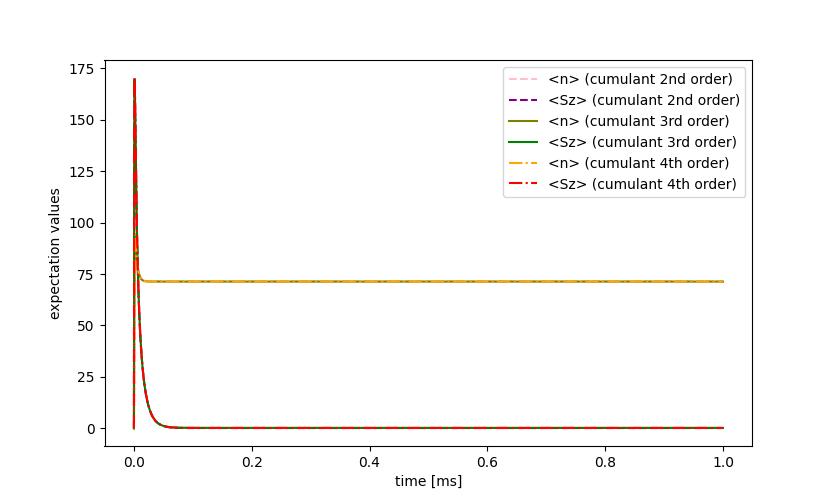
\includegraphics[width=1\linewidth]{10k_234_nsz}
  \caption{Original plot with full time interval (0 to 1ms)}
\end{subfigure}%
\hspace{1em}%
\begin{subfigure}{.48\textwidth}
  \centering
  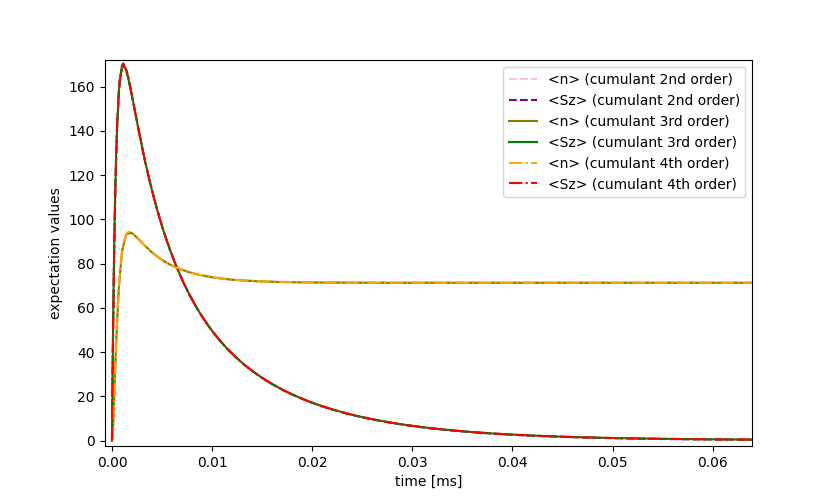
\includegraphics[width=1\linewidth]{10k_234_nsz_zoom_1}
  \caption{Zoom on the main features (from 0 to 60µs).}
  \label{10k_234_nsz_zoom_1}
\end{subfigure}
\caption{Simulation results for 10,000 atoms inside the cavity. Three set of equations are generated with order $m=2$ (denoted "2nd order"), $m=3$ (denoted "3rd order") and $m=4$ (denoted "4th order"). Two types of expectation values are plotted: the photon number $\left\langle \hat{n} \right\rangle$ inside the cavity and the atomic inversion $\left\langle  \hat{S}_z \right\rangle$}
\end{figure}

\begin{figure}[h!]
\centering
\begin{subfigure}{.48\textwidth}
  \centering
  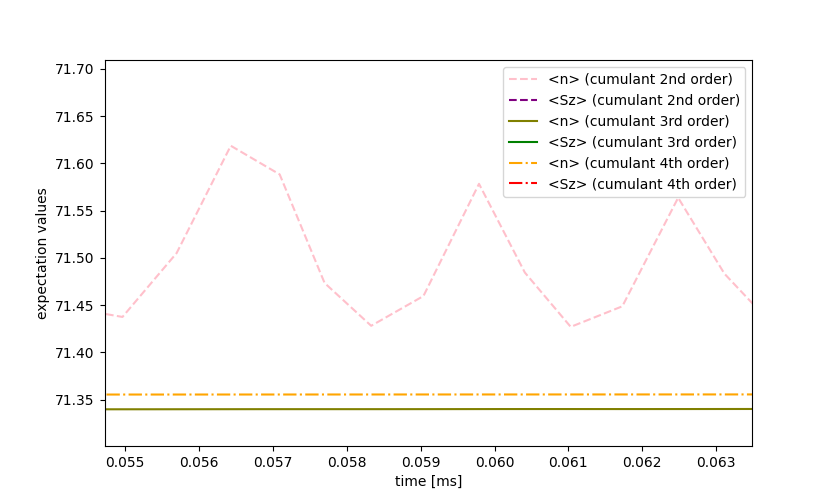
\includegraphics[width=1.1\linewidth]{10k_234_nsz_zoom_2}
  \caption{Steady-state of $\left\langle \hat{n} \right\rangle$. Pink dotted curve is of 2nd order. Olive solid curve is of 3rd order. Orange dot-dashed is of 4th order. The second order shows clear unstabilities at steady-state.}
  \label{fig:steady-2nd-unstable}
\end{subfigure}%
\hspace{1em}%
\begin{subfigure}{.48\textwidth}
  \centering
  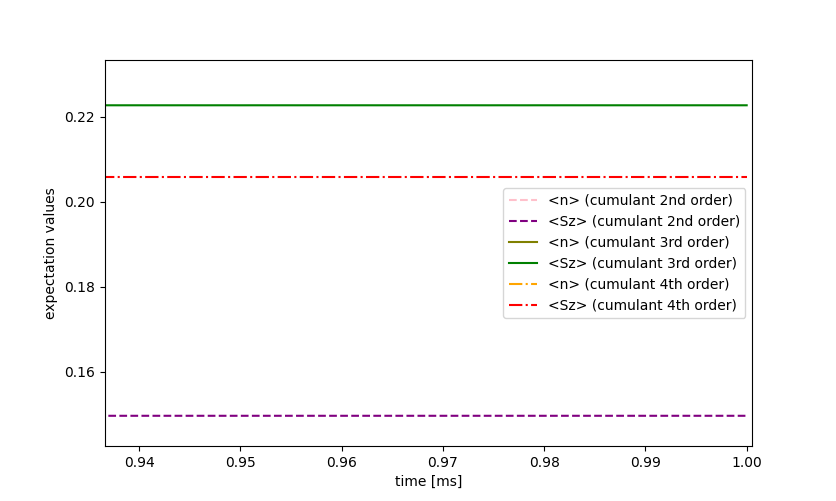
\includegraphics[width=1\linewidth]{10k_234_nsz_zoom_3}
  \caption{Steady-state of $\left\langle \hat{S}_z \right\rangle$. Purple dotted curve is of 2nd order. Green solid curve is of 3rd order. Red dot-dashed is of 4th order. We take the thrid order curve as the limit $\left\langle \hat{S}_z(t_\infty) \right\rangle$}
\end{subfigure}
\caption{Zoom on the convergent steady-state values for 10,000 atoms inside the cavity.}
\end{figure}

\begin{figure}[h!]
\centering
\begin{subfigure}{.48\textwidth}
  \centering
  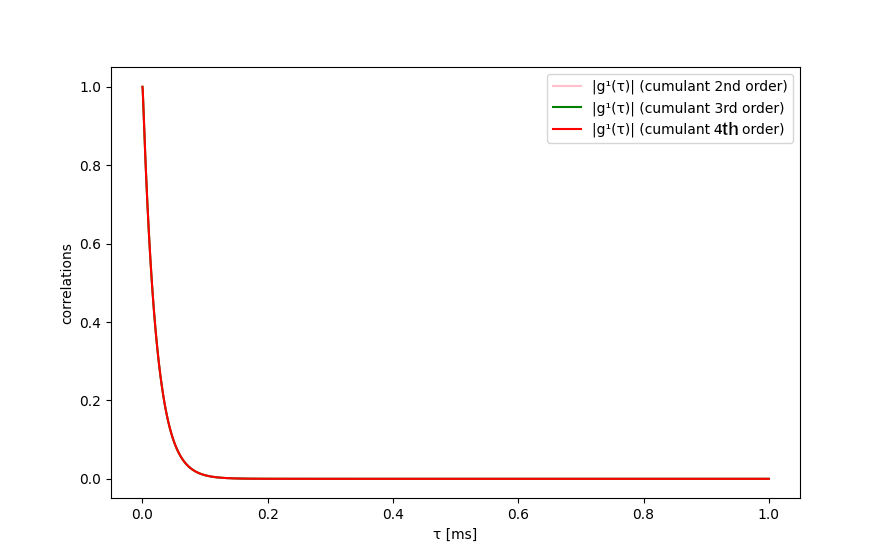
\includegraphics[width=1\linewidth]{10k_234_g1}
  \caption{Original plot with full time interval (0 to 1ms).}
\end{subfigure}%
\hspace{1em}%
\begin{subfigure}{.48\textwidth}
  \centering
  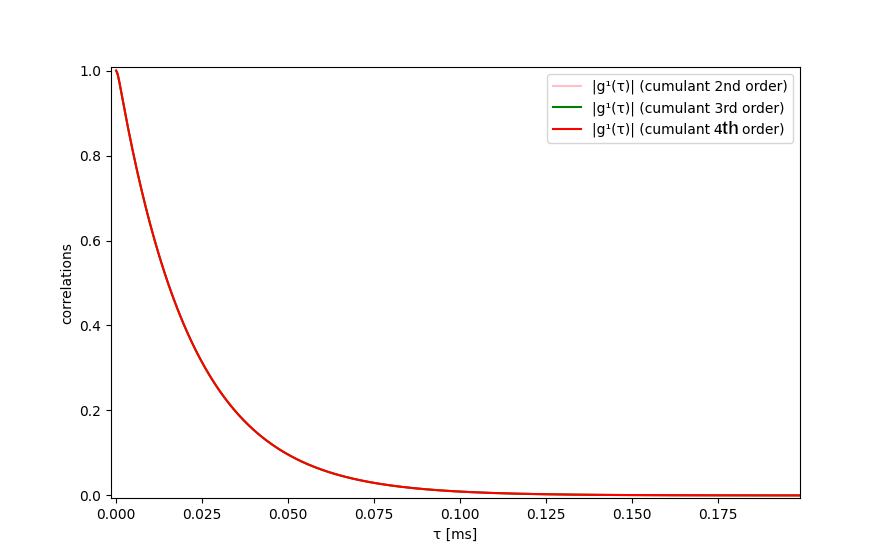
\includegraphics[width=1\linewidth]{10k_234_g1_zoom}
  \caption{Zoom on the main feature (from 0 to 175µs).}
  \label{10k_234_g1_zoom}
\end{subfigure}
\caption{Simulation results for 10,000 atoms inside the cavity. Plot of $\vert g^1(\tau) \vert$. The three sets clearly overlap and the last rendered curve is shown of top of the others (namely, the 4th order in solid red).}
\end{figure}

\begin{figure}[h!]
\caption{Extra zoom of $\vert g^1(\tau) \vert$ for 10,000 atoms inside the cavity. It is evident that showing the 2nd, 3rd or 4th order of the solution doesn't affect the results (or not enough to be considered).}
\centering
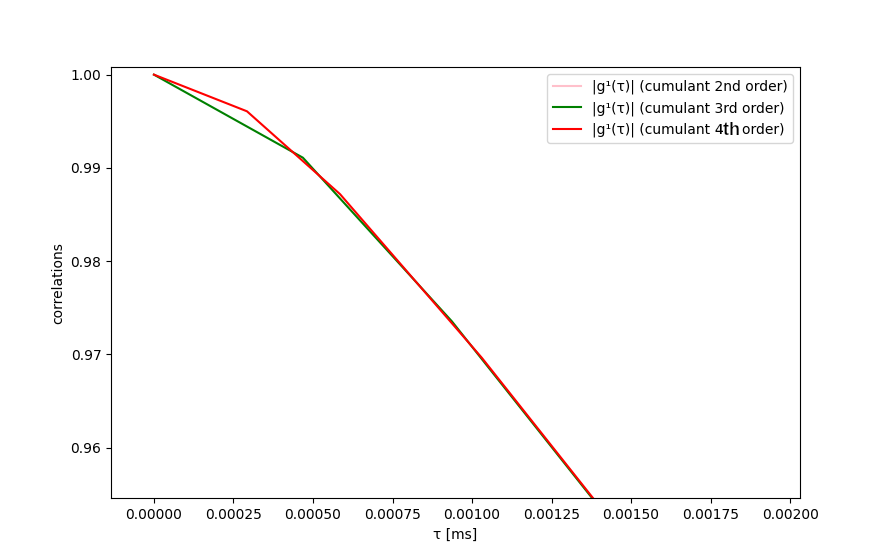
\includegraphics[width=0.6\textwidth]{10k_234_g1_zoom_2}
\end{figure}

\pagebreak
\subsection{Simulation with 100,000 atoms inside the cavity}

Then, we set $N=100,000$. Thus, the initial state is $\ket{j=50,000, m=0, n=0}$. The repump rate is evaluated to $\nu \simeq \kappa / 103.9537874$. The steady state shows $\left\langle \hat{S}_z(t_\infty) \right\rangle \sim 2$: the ratio is $0.50002$.

\begin{figure}[h!]
\centering
\begin{subfigure}{.48\textwidth}
  \centering
  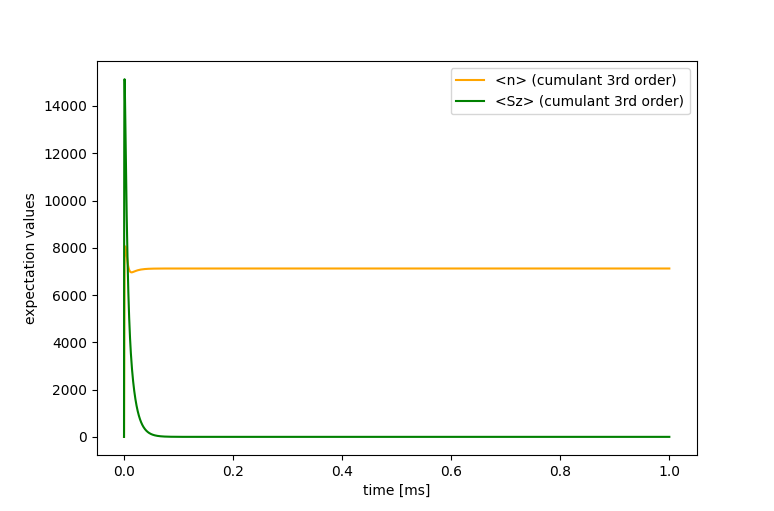
\includegraphics[width=1\linewidth]{100k_3_nsz}
  \caption{Original plot with full time interval (0 to 1ms)}
\end{subfigure}%
\hspace{1em}%
\begin{subfigure}{.48\textwidth}
  \centering
  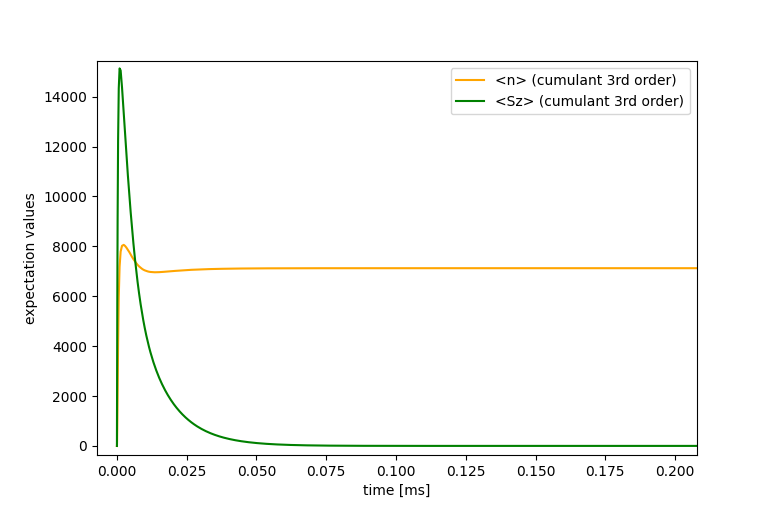
\includegraphics[width=1\linewidth]{100k_3_nsz_zoom_1}
  \caption{Zoom on the main features (from 0 to 200µs).}
  \label{100k_3_nsz_zoom_1}
\end{subfigure}
\caption{Simulation results for 100,000 atoms inside the cavity. Two types of expectation values are plotted: the photon number $\left\langle \hat{n} \right\rangle$ inside the cavity (green) and the atomic inversion $\left\langle  \hat{S}_z \right\rangle$ (orange)}
\end{figure}

\begin{figure}[h!]
\centering
\begin{subfigure}{.48\textwidth}
  \centering
  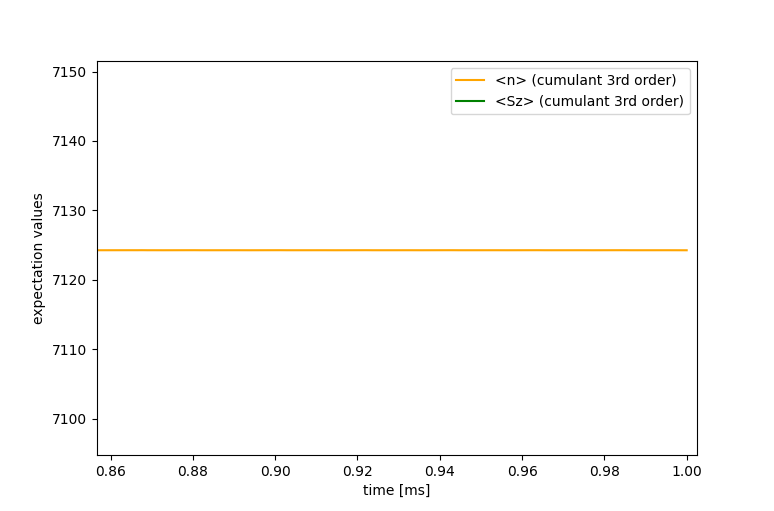
\includegraphics[width=1\linewidth]{100k_3_nsz_zoom_3}
  \caption{Steady-state of $\left\langle \hat{n} \right\rangle$.}
\end{subfigure}%
\hspace{1em}%
\begin{subfigure}{.48\textwidth}
  \centering
  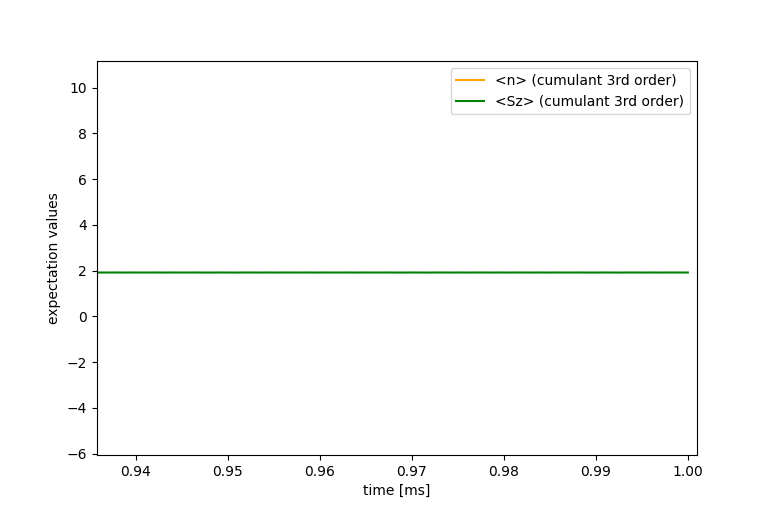
\includegraphics[width=1\linewidth]{100k_3_nsz_zoom_2}
  \caption{Steady-state of $\left\langle \hat{S}_z \right\rangle$.}
\end{subfigure}
\caption{Zoom on the convergent steady-state values for 100,000 atoms inside the cavity.}
\end{figure}

\begin{figure}[h!]
\centering
\begin{subfigure}{.48\textwidth}
  \centering
  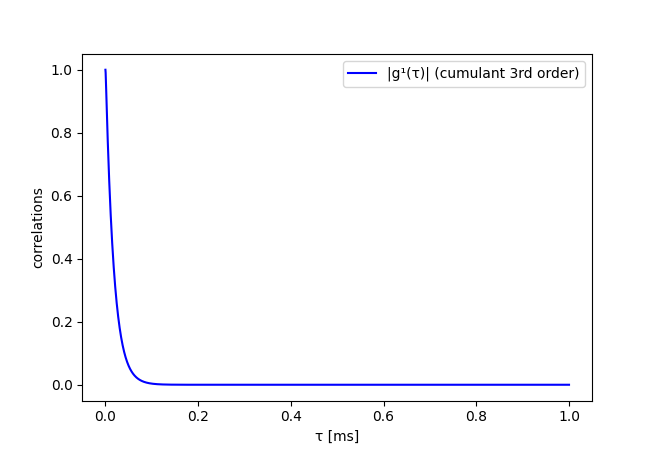
\includegraphics[width=1\linewidth]{100k_3_g1}
  \caption{Original plot with full time interval (0 to 1ms).}
\end{subfigure}%
\hspace{1em}%
\begin{subfigure}{.48\textwidth}
  \centering
  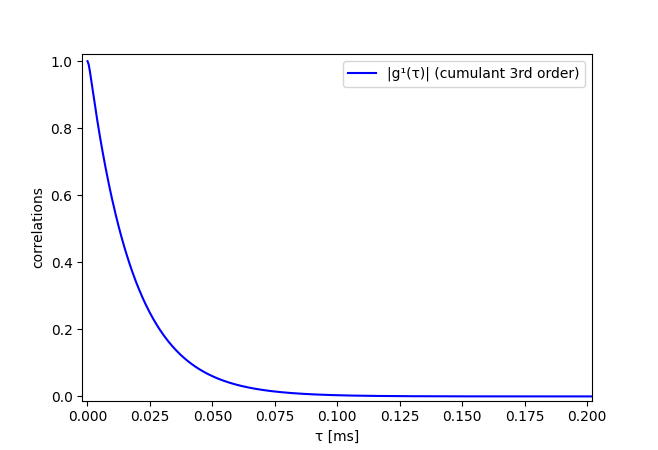
\includegraphics[width=1\linewidth]{100k_3_g1_zoom_1}
  \caption{Zoom on the main feature (from 0 to 200µs).}
  \label{100k_3_g1_zoom_1}
\end{subfigure}
\caption{Simulation results for 100,000 atoms inside the cavity. Plot of $\vert g^1(\tau) \vert$.}
\end{figure}

\pagebreak
\subsection{Simulation with 300,000 atoms inside the cavity}

Finally, we set $N=300,000$. We start to see on the figures some clear oscillations due to the high numbers stored in memory (i.e the stability is progressively lost as the number of atoms increases). This is the highest $N$ which gives coherent results with the  Thus, the initial state is $\ket{j=150,000, m=0, n=0}$. The repump rate is evaluated to $\nu \simeq \kappa / 103.954651$. The steady state shows $\left\langle \hat{S}_z(t_\infty) \right\rangle \sim 5.6$. : the ratio is approximately $0.5000187$.

\begin{figure}[h!]
\centering
\begin{subfigure}{.48\textwidth}
  \centering
  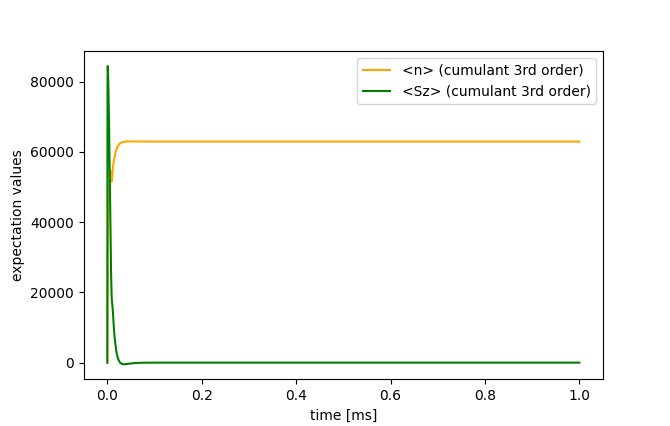
\includegraphics[width=1\linewidth]{300k_3_nsz}
  \caption{Original plot with full time interval (0 to 1ms)}
\end{subfigure}%
\hspace{1em}%
\begin{subfigure}{.48\textwidth}
  \centering
  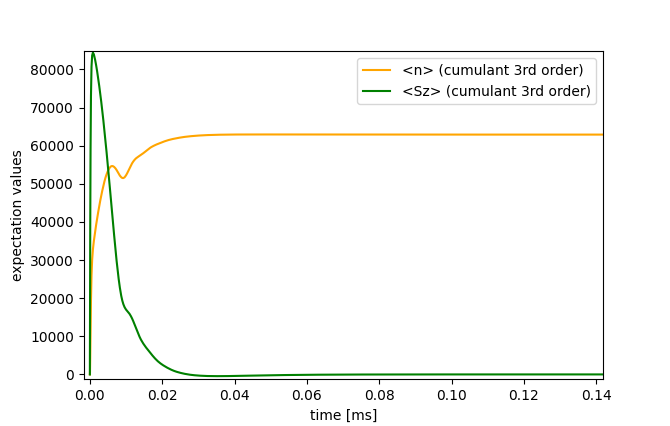
\includegraphics[width=1\linewidth]{300k_3_nsz_zoom_1}
  \caption{Zoom on the main features (from 0 to 140µs).}
  \label{300k_3_nsz_zoom_1}
\end{subfigure}
\caption{Simulation results for 300,000 atoms inside the cavity. Two types of expectation values are plotted: the photon number $\left\langle \hat{n} \right\rangle$ inside the cavity (green) and the atomic inversion $\left\langle  \hat{S}_z \right\rangle$ (orange)}
\end{figure}

\begin{figure}[h!]
\centering
\begin{subfigure}{.48\textwidth}
  \centering
  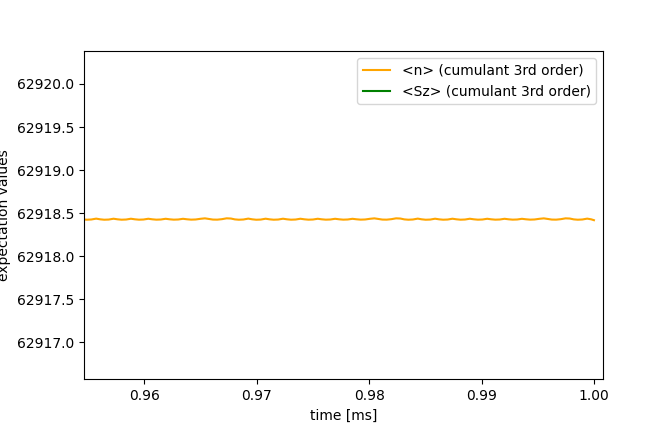
\includegraphics[width=1\linewidth]{300k_3_nsz_zoom_3}
  \caption{Steady-state of $\left\langle \hat{n} \right\rangle$.}
\end{subfigure}%
\hspace{1em}%
\begin{subfigure}{.48\textwidth}
  \centering
  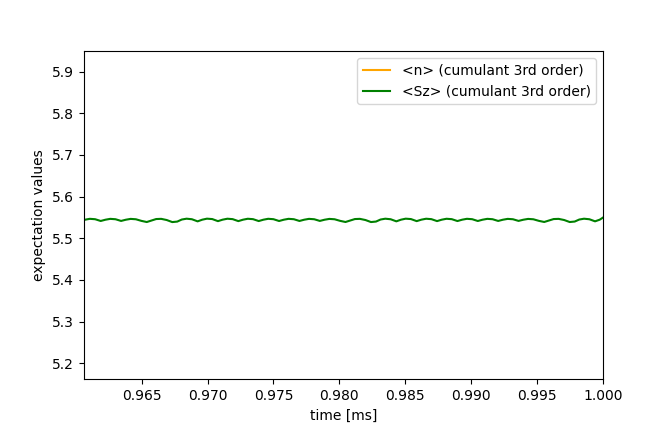
\includegraphics[width=1\linewidth]{300k_3_nsz_zoom_2}
  \caption{Steady-state of $\left\langle \hat{S}_z \right\rangle$.}
\end{subfigure}
\caption{Zoom on the convergent steady-state values for 300,000 atoms inside the cavity. We clearly see unstability of the solution by the small oscillations at "steady-state". Compared to the 2nd order in figure \ref{fig:steady-2nd-unstable} where the unstabilities were due to the lack of quantum correlation in the set of equations, here the unstability is due to the numerical values starting to exceed the float precision.}
\end{figure}

\begin{figure}[h!]
\centering
\begin{subfigure}{.48\textwidth}
  \centering
  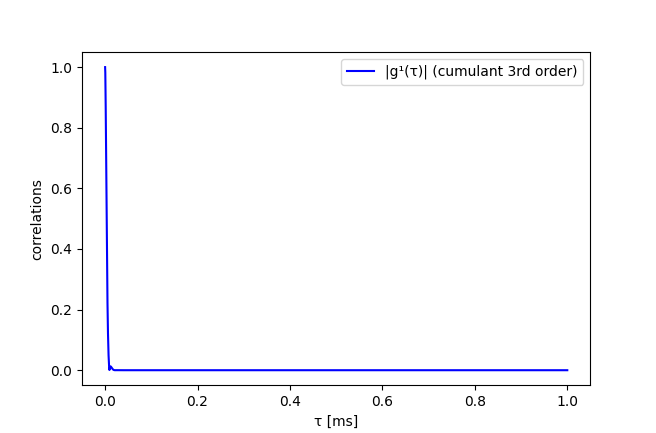
\includegraphics[width=1\linewidth]{300k_3_g1}
  \caption{Original plot with full time interval (0 to 1ms).}
\end{subfigure}%
\hspace{1em}%
\begin{subfigure}{.48\textwidth}
  \centering
  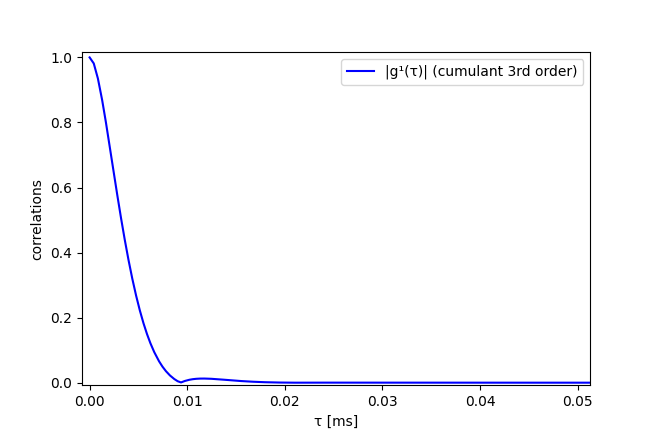
\includegraphics[width=1\linewidth]{300k_3_g1_zoom_1}
  \caption{Zoom on the main feature (from 0 to 50µs).}
  \label{300k_3_g1_zoom_1}
\end{subfigure}
\caption{Simulation results for 300,000 atoms inside the cavity. Plot of $\vert g^1(\tau) \vert$.}
\end{figure}

\pagebreak
\subsection{Discussion}

First of all, we can notice that we respect for the three cases the experimental condition of having approximately half of the atoms excited \footnote{And this proportion of excitation is kept almost constant across the three cases}. Moreover, as we shall see in chapter \ref{data_analysis_chapter}, the quantum system emits a a small additional burst of light in the first 10µs before reaching the steady-state for the two first cases (10,000 and 100,000) in figures \ref{10k_234_nsz_zoom_1} and \ref{100k_3_nsz_zoom_1}. This behavior corresponds excatly to the experimental signal. The behavior of the third case does not show an equivalent burst in figure \ref{300k_3_nsz_zoom_1} which gives a clue of its inaccuracy.\footnote{There is one oscillation in the same interval of time but it is not superior in value to the steady-state: this is not a burst.}

In order to compute the coherence time $\tau_c$, we integrate over:
\begin{equation}
\label{half_tau_c_loudon_def}
\int_{0}^{+\infty} \vert g_1(\tau) \vert^2 \, d\tau
\end{equation}
and make use of the relation $g^1(\tau)=g^1(-\tau)$ by doubling the result of \ref{half_tau_c_loudon_def} to obtain \ref{tau_c_loudon_def}. In that way, we get $\tau_c \simeq 22$µs for 10,000 atoms inside the cavity, $\tau_c \simeq 19$µs for 100,000 atoms, $\tau_c \simeq 4.8$µs for 300,000 atoms. We can notice that from 10,000 to 100,000 atoms, the number of atoms is multiplied by 10 (an order of magnitude higher) whereas the coherence time $\tau_c$ is reduced by 10-15\%. However, from 100,000 to 300,000 atoms, the number of atoms is multiplied by 3 (same order of magnitude) whereas the coherence time $\tau_c$ if almost divided by 4. Moreover, thanks to the re-evaluation of the repump rate $\nu$ and the computation of the ratio \ref{special_ratio}, we kept track of the equivalence of the atom excitation value which was somehow identical in proportion for the three cases of atoms inside the cavity. In other words, this difference in the reduction of $\tau_c$ does not come from the position of the Bloch vector of the system on the Block sphere. Nevertheless, for the difference of $\tau_c$ between 10,000 and 300,000 atoms, we can suspect the high amount of atoms as problematic for the float precision which \textit{collapses} the numerical solution.

Although the coherence time is not quite respected as we shall see in chapter \ref{data_analysis_chapter}, it is clear that $\vert g^1(\tau) \vert$ does not exhibit a lorentzian behavior for the cases 10,000 and 100,000 atoms in figures \ref{10k_234_g1_zoom} and \ref{100k_3_g1_zoom_1}. The third case shows a clear gaussian shape in figure \ref{300k_3_g1_zoom_1} but can be biased as we got some clues of the numerical unstability of the system for this case.

\chapter{Heterodyne experiment}
\section{Standard setup for $g^1$ and its limitations}

In this section, we shall describe a standard method of measuring the frist order correlation function of a given classical electric field. This is meant to introduce some concepts of wave mixing, intensity detection and noise limit. Some detection properties are limited in the present case and this give a justification of the setup used in the actual experiment for measuring $g^1$.

Firstly, let's consider a linearly poilarized electric field $E_1(x, t)$ in its phasor representation as in equation \eqref{eq1} where we droped the vector sign as the field can be described only by its amplitude. Note that at this point, we do not make any hypothesis about the frequencies bearing by this field except that the field is quasi-monochromatic (i.e the linewidth of the emited light is not null around the main frequency beat). This field is our field of interest, that is to say, we want to extract coherence information from it. Thereby, we mix it with another field $E_2(x, t)$ which trivially gives a total field of:
\begin{equation}
\label{e_tot_def}
E_{total} = E_1 + E_2
\end{equation}
Now, we place a detector at $x=0$ relatively to the total field. However, to highlight the phase difference from a field to another at the detector, we write the second electric field with a time delay $\tau$. In the classical view, the role of the detector is to transform a mean light intensity (i.e an amount of photon) into an electric intensity (i.e an amount of electron). With certain hypothesis \footnote{See section ?? (Data analysis)} one may approximate the intensity as:
\begin{align}
\begin{split}
I_{total}(t, \tau) \simeq \vert\overline{E}_{total}(t)\vert^2 &= (\overline{E}_1(t) + \overline{E}_2(t + \tau))(\overline{E}_1^*(t) + \overline{E}_2^*(t + \tau))\\
&= \vert \overline{E}_1(t) \vert^2 + \vert \overline{E}_2(t + \tau) \vert^2 + 2\Re\left\lbrace \overline{E}_1(t)\overline{E}_2^*(t + \tau)\right\rbrace
\end{split}
\end{align}
that we may rewrite for simplicity:
\begin{equation}
I_{total}(t, \tau) = I_1(t) + I_2(t + \tau) + 2\Re\left\lbrace \overline{E}_1(t) \overline{E}_2^*(t + \tau)\right\rbrace
\end{equation}
where the approximation sign is implicit.

Then, we assume that the dectector transfer exactly $100\% $ of the received light into the eletric wire (i.e quantum efficiency $\eta = 1$) and that the collected intensity is the mean value of the total intensity for an interval of time $T$:
\begin{equation}
I_{detected}(\tau) \stackrel{\text{def}}{=} \left\langle I_{total}(t) \right\rangle_T = \left\langle I_1(t) \right\rangle_T + \left\langle I_2(t + \tau) \right\rangle _T + 2\left\langle \Re\left\lbrace \overline{E}_1(t) \overline{E}_2^*(t + \tau)\right\rbrace \right\rangle _T
\end{equation}
with:
\begin{equation}
\left\langle \cdot \right\rangle _T = \int_T \cdot \,\,dt
\end{equation}

We introduce the correlation variable:
\begin{equation}
\label{gamma_corr_def}
\gamma_{1,2}(\tau) \stackrel{\text{def}}{=} \frac{\left\langle E_1(t) E_2^*(t + \tau) \right\rangle _T}{\sqrt{\left\langle I_1(t) \right\rangle_T \left\langle I_2(t + \tau) \right\rangle _T }} \in \mathbb{C}
\end{equation}
This previous definition transforms $I_{detected}$ as:
\begin{equation}
I_{detected}(\tau) = I_1 + I_2 + 2\sqrt{I_1 I_2} \Re \left\lbrace \gamma_{1,2}(\tau) \right\rbrace
\end{equation}
where we interchanged $\Re \left\lbrace \cdot \right\rbrace$ with $\left\langle \cdot \right \rangle$ \footnote{In other words, the mean value of the real part is equivalent to the real part of the mean value, by linearity.} and where we dropped the time dependences of the intensity terms (from integration, those terms becomes constant according to the time $t$).
By its normalization factor (i.e the denominator in \eqref{gamma_corr_def}), one may say that the norm of gamma is included between $0$ and $1$ where $0$ holds for complete incoherence whereas $1$ holds for full coherence. This means that we can write two extrema:
\begin{align}
I_{detected, max} &= I_1 + I_2 + 2\sqrt{I_1 I_2} \vert \gamma_{1,2} \vert\\
I_{detected, min} &= I_1 + I_2 - 2\sqrt{I_1 I_2} \vert \gamma_{1,2} \vert
\end{align}
Moreover, we define a last variable $\nu$ called the \textit{visibility}\footnote{Sometimes, $\nu$ is named the \textit{fringes visibility} in order to recall the periodicity involved in interference experiments.}:
\begin{align}
\label{def_visibility}
\nu \stackrel{\text{def}}{=} \frac{I_{max} - I_{min}}{I_{max} + I_{min}}
\end{align}
which represents the maximal contrast that one may observe for an intensity signal. From the dectector point of view, that is to say, the visibility of the electric signal after the wire reads:
\begin{align}
\nu = \frac{I_{detected, max} - I_{detected, min}}{I_{detected, max} + I_{detected, min}} = \frac{2\sqrt{I_1 I_2} \vert \gamma_{1,2} \vert}{I_1 + I_2}
\end{align}
In other words, the visibility two mixed electric field is proportional to the coherence term $\left\langle E_1(t) E_2^*(t + \tau) \right\rangle _T$.

Now, we make two final hypothesis:
\begin{itemize}
	\item The second electric field is coming from the same source as the first one: $E_1 = E_2 = E$. However, the two field are still delayed from each other by a time $\tau$. Experimentally, this may be reproduced with a simple Michelson interferometer which allows to vary the delay thanks to the difference of the optic path length of the two arms.
	\item The mean value of the total intensity $I_{total}$ is constant over the time. This assumption is not necessarily obvious in a sense that our previous development could involve pulses of light, gaussian envelopes, etc. However this hypothesis lets us write that the detected intensity does not vary with time, hence the mean of interval lengths $T$ taken at  different origins give the same value: $\left\langle I(t) \right\rangle_T = \left\langle I(t + \tau) \right\rangle _T$.
\end{itemize}
At the end of the day, we obtain:
\begin{equation}
\nu = \vert \gamma_{1, 2} \vert = \frac{\vert\left\langle E(t) E^*(t + \tau) \right\rangle _T\vert}{\vert I \vert} = \vert g^1(\tau) \vert
\end{equation}
that is to say, for a quasi-monochromatic input field, the detection of the output field of a Michelson interferometer produces a detected intensity through the connected oscilloscope which, after maths done, gives the norm of the first order correlation function. Then, varying the path length difference allows to sketch the norm of $g^1$ according to the time delay $\tau$. It is important to notice that if we set:
\begin{equation}
I_{detected}(\tau) \stackrel{\text{def}}{=} \eta \left\langle I_{total}(t) \right\rangle_T
\end{equation}
Then, when defining the visbility in \eqref{def_visibility}, the quantum efficiency vanishes equally through the division. In other words, measuring $g^1$ in this way is not dependent on the dectector efficiency: loosing photons at the arrival does not change the statistics with the visibility approach.

However, although the Michelson interferometer is a simple setup which gives nicely $g^1$, this method suffer from three major incovenients:
\begin{itemize}
	\item The detector must follow the frequency of the input field: as we are overlapping the same field (i.e the same frequency), the resulting field gives only component of null, same or twice the original frequency. In other words, as the actual experiment works with lasers involving a few hundreds of THz, our detector must follow those frequencies. No real dectector can achieve it in those days.\footnote{Actually, the detector is able to show the mean intensity value, that is to say a DC signal, in the presence of \textit{any} light (depending on the specification). However, because of the \textit{dead time} and other technical reasons, modern detectors are not able to follow the high frequency variations of orders of THz.}
	\item As the theory is facing experiment, it is worth to notice that the detector \textit{always} has a specific range of possible power inputs. In other words, for to low or to high laser power, the detector does not send any electric signal, which is critical for the first case as the cavity output gives superradiant lasing of a few nano watts.
	\item This configuration is highly sensitive to the noise. Indeed, any variation in the detected intensity is concidered as a variation from the electric field, thus, a variation for $g^1$. However, those variations are not necessarily only representative of the output field generated by the quantum system but also by other external perturbations called \textit{noise} which can be classical (electric current noise for example) or quantum\footnote{The quantum noise is not directly related to the quantum system in itlsef but by the fundamental photon statistics generated from the system.}.
\end{itemize}

At the end of the day, this setup turns out to not be optimal for rigorous and/or advanced measurements. Therefore, the next section shall present another approach as well as the basic concept involved in order to solve the three previous inconvenients.

\section{Balanced heterodyne setup}

An heterodyne setup is, as stated by its name, an experiment involving two mixed electric fields of \textit{different} frequencies\footnote{"Hetero" is the Greek prefix meaning "irregularity" and "dyne" suffix for "dynamic" in contrary to "homo" (= "same") for a homodyne setup with equal frequencies.} which are collected by two detectors. The electric current produced by both detected intensity, that we call \textit{photocurrent}, is then substracted and the resulting electric signal can be recorded on an oscilloscope for example. 

A simple version of the heterodyne setup used in the actual experiment is summarysed in figure \ref{fig:heterodyne-fst}.

\begin{figure}[h!]
\caption{Heterodyne setup diagram.}
\centering
\includegraphics[width=\textwidth]{heterodyne-fst}
\label{fig:heterodyne-fst}
\end{figure}

\begin{itemize}
 \item $\vv{E}_{cav}$ is the electric field generated at the ouput of the cavity.
 \item $\vv{E}_{LO}$ stands for the electric field named the \textit{local oscillator} and sometimes abbreviated as the \textit{reference} laser. Its frequency diverges from the cavity field frequency. It is in general emited from a laser and hence is concidered as \textit{nearly}\footnote{$\vv{E}_{LO}$ cannot be perfectly coherent from an experimental point of view but we consider it as such in the theoretical developement.} perfectly coherent source.
 \item The beam splitter essentially mix the input fields in a way described in section ?? (Data analysis) which roughly gives, as outputs, the added or substracted input fields.
\end{itemize}

In order to show the different frequency components involved into the detected intensity, we mix the two E-fields as in \eqref{e_tot_def} with the following definitions:
\begin{align}
\label{e_cav_e_lo}
\begin{split}
\vv{E}_{cav}(t) &=\frac{\vv{E}_{cav}}{2} e^{i\omega_{c}t} + \frac{\vv{E}_{cav}}{2} e^{-i\omega_{c}t} \\
\vv{E}_{LO}(t) &= \frac{\vv{E}_{LO}}{2} e^{i\omega_{LO}t} + \frac{\vv{E}_{LO}}{2} e^{-i\omega_{LO}t}
\end{split}
\end{align}that is to say, we consider $\vv{E}_{cav}(t)$ as perfectly coherent (i.e monochromatic) and we omit the phase difference, the whole for the sake of simplicity as the excpected result effects would be similar in case of phase unmatch and quasi-monochromatic cavity field. Note that $\vv{E}_{cav/LO}$ without the time dependence $t$ is the \textit{vector}-amplitude of the respective field (i.e a constant vector). Now appling the exact formula:
\begin{equation}
I_{total}(t) = \vv{E}_{total}(t)^2 = \left(\vv{E}_{cav}(t) + \vv{E}_{LO}(t)\right) \cdot \left(\vv{E}_{cav}(t) + \vv{E}_{LO}(t)\right)
\end{equation} 
one gets four different terms:
\begin{align}
I_{total,a}(t) &= \vert\vv{E}_{cav}\vert^2\left(1 + \cos(2\omega_{cav}t)\right)\\
I_{total,b}(t) &= \vert\vv{E}_{LO}\vert^2\left(1 + \cos(2\omega_{LO}t)\right)\\
I_{total,c}(t) &= \vv{E}_{cav}\cdot\vv{E}_{LO}\cos\left((\omega_{cav} - \omega_{LO})t\right)\\
I_{total,d}(t) &= \vv{E}_{cav}\cdot\vv{E}_{LO}\cos\left((\omega_{cav} + \omega_{LO})t\right)
\end{align}
where $I_{total}(t) = I_{total,a}(t) + I_{total,b}(t) + I_{total,c}(t) + + I_{total,d}(t)$.

The experiement is configured as the input electric fields being linearly and parallely polarized: so we consider $\vv{E}_{cav}$ and $\vv{E}_{LO}$ as such. This simplifies the equation by only taking into account the amplitude of the fields instead of their vector components. Also, as the intensity calculation involve a scalar product of the electric vector fields, the collinear polarization allows to maximise the light power when mixing two E-fields. We obtain:
\begin{align}
I_{total,a}(t) &= E_{cav}^2\left(1 + \cos(2\omega_{cav}t)\right)\\
I_{total,b}(t) &= E_{LO}^2\left(1 + \cos(2\omega_{LO}t)\right)\\
\label{mix_hetero_ic}
I_{total,c}(t) &= E_{cav}E_{LO}\cos\left((\omega_{cav} - \omega_{LO})t\right)\\
\label{mix_hetero_id}
I_{total,d}(t) &= E_{cav}E_{LO}\cos\left((\omega_{cav} + \omega_{LO})t\right)
\end{align}

In other words, the detected intensity, which is propotional to the total intensity, has four \textit{beat mode} as one would see on a spectrum analyzer: $2\omega_{cav}$, $2\omega_{LO}$, $\omega_{cav} - \omega_{LO}$ and $\omega_{cav} + \omega_{LO}$. As stated in the previous section, the cavity frequency is in order of THz, which is undetectable for a realistic detector. Now, if we set the frequency of the local oscillator of the same order of magnitude as $\omega_{cav}$ but \textit{slightly} shifted with $\omega_{LO} = \omega_{cav} + \delta\omega$ and $\delta\omega$ is a frequency belonging to the bandwidth of the detector, then we get again four beats:
\begin{equation}
\label{list_comp_light_mix}
2\omega_{cav}, \quad\quad 2\omega_{cav} + 2\delta\omega, \quad\quad \delta\omega, \quad\quad 2\omega_{cav} + \delta\omega
\end{equation}
The only detected beat is $\delta\omega$ as all the others are of order of $2\omega_{cav}$ (i.e in few hundreds of Thz). Thereby, the detector is sensitive to the frequency variations of $I_{total,c}(t)$ only. Moreover, this is not the only advantage of adding a local oscillator. Indeed, one may notice that the intensity term \eqref{mix_hetero_ic} is dependent to the amplitude of the cavity field \textit{and} the amplitude of the local oscillator. In that way, we are able to tune the total light intensity observed and face the problem of low power from the cavity field: the local oscillator is a well controlled laser and if, for example, the $E_{cav}$-field power is in order of picowatts (i.e well below the range of detected power), it is enough to power up the reference laser in order to detect the expected beat again.

Finally, the principle of photocurrent substraction is called a balanced detection. As we substract the two photocurrent, the resulting electric signal should be null in the case where both fields are equal. In that way, a very samll variation in one arm should give a non-null signal: this setup is extremely sensitive to small variations. However, even with the exact same field hitting both diodes of the dectector, some noise still resides. We distinguish two types of noise:
\begin{itemize}
	\item The shot noise: it reflects the statistical randomness of the light and is only dependent on the quantum uncertainties of the photons. That is why, it is often called equivalently \textit{quantum noise}. For Poissonian distribution of the photons (i.e for classical light) the photocurrent noise is also amplified and is linearly dependent to the mean intensity light\footnote{See section 2.5}.. For sub-Poissonian lights, where the photons are anti-bunched, it is possible to detect light below the shot noise limit (which is defined by the classical limit of detection for Poissonian light)\footnote{See Fox ??}.
	\item The eletrical noise: all the electric component induces a white noise into the resulting signal which is inner to the way the detector is manufactured.
\end{itemize} 
Those two types of noises are uncorrellated and just add together while the amplification through the circuit, naturally increases those two noises. 

Thus, the idea behind balanced detection is to cancel the classical noise which can randomly appear on both diodes of the detector at the same time. Indeed, if any correlated variation of the signal apperas in both emited photocurrent, the substraction \textit{erases} this correlated variation (i.e noise) in a sense that the resulting signal then owns the quantum noise, the uncorrelated photocurrent noise (which may be amplified) as well as the electric noise (which is a white noise, hence uncorrelated). Nevertheless, the remaining noise may be considered as very small for our purpose and the detector is made in order to reduce the electrical and amplified power noise in the bandwidth of interest. This reduction of noise by electronic design is the subject of the next section.

\section{Balanced low-noise detector}

In theory, the electronic circuit does not produce any additional noise. That is to say, if there is any variation of the photocurrent at the entry of the circuit, thus after the diodes, the output noise corresponds to this variation (except the amplification of the noise which is a side effect from the purpose of the circuit). In a real world however, without any photocurrent input, the exit cable of the detector shows a random ouput voltage. Of course, the detector must be under voltage, otherwise, no ouput can be generated as some essential components need an external source of electric power. Moreover, this electrical noise being evaluated in term of power (dBm), is a critical parameter. Indeed, if the shot noise limit is lower than the electrical noise, it is possible to lose some part of the data, especially the very weak quantum correlations. Therefore, it is essential to reduce the electrical noise generated by the internal components as much as possible.

Firstly, we introduce a basic diagram on the working principle of the detector in figure \ref{fig:detector-fst}. It is mainly composed of two diodes (block (1)), which are also called \textit{photodiodes} as they react to the incoming light, plus an essential circuit called \textit{transimpedance amplifier} (block (2)) connected in between of the diodes.

\begin{figure}[h!]
\caption{Basic electric circuit showing the working principle of the detector.}
\centering
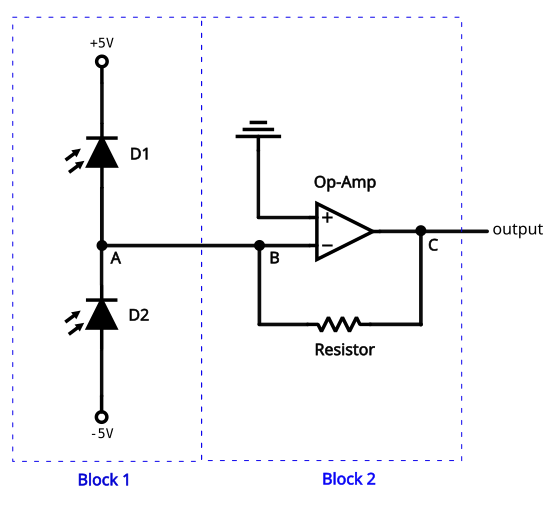
\includegraphics[width=0.6\textwidth]{detector-fst}
\label{fig:detector-fst}
\end{figure}

The photodiodes are placed in the so called \textit{photoconductive mode} where the region of reverse bias in figure \ref{fig:photodiode-vi} defines the relation bewteen the voltage and the current. In fact a basic diode, by principle, allows the current to flow through it only if the voltage is positive on the cathode and negative on the anode (i.e forward bias). Otherwise, when reverse biased, the current does not flow\footnote{In practice, there exists a a certain voltage called \footnote{breakdown voltage} where the current suddenly flow exponentially from the anode to the cathode.}. For a photodiode, the same idea applies except that when reverse biased, the current can flow through it only if the diode is illuminated. Note that even if the current flows, the difference of voltage between the anode and cathode stays the same: in other words, the photodiode does not act as a switch where the the voltage is homogeneous through the component when the current flow (i.e when the circuit is closed). 

\begin{figure}[h!]
\caption{Photodiode modes according the the applied voltage and light intensity.}
\centering
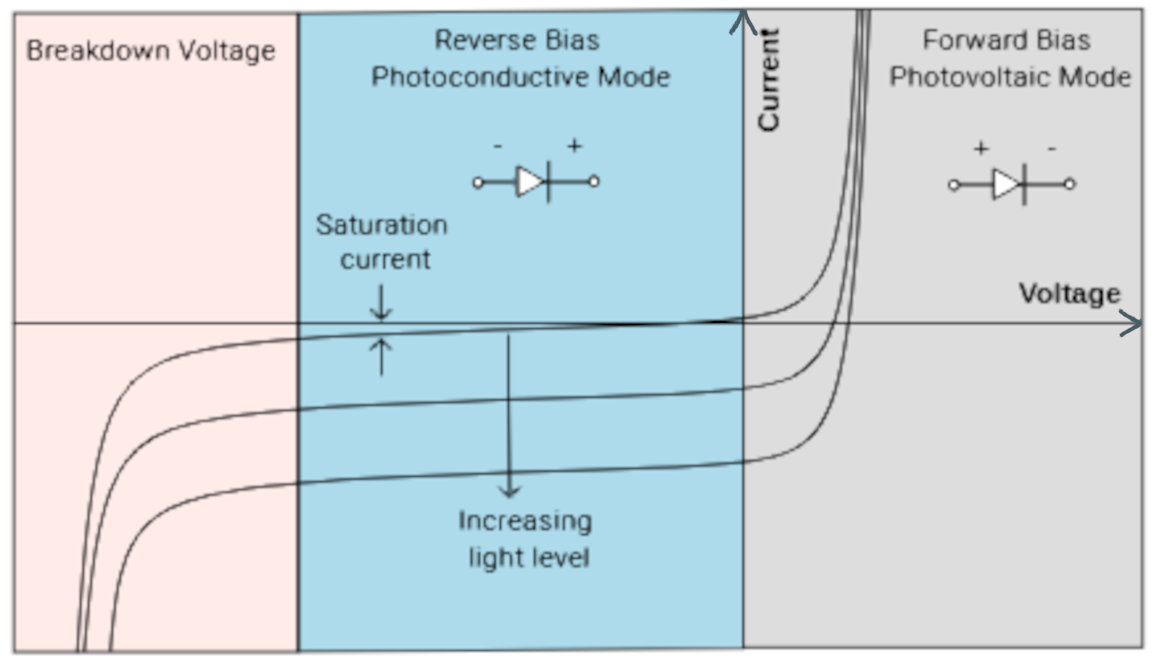
\includegraphics[width=0.7\textwidth]{photodiode-vi}
\label{fig:photodiode-vi}
\end{figure}

Thereby, if we isolate the block (1), the current flows through the positive voltage (+) above the first diode (D1), to the negative voltage (-) under the second diode (D2) when both photodiodes are illuminated. In that case, by Kirchhoff's current law, no current can flow through (A) to (B). Otherwise, we can distinguish two cases:
\begin{itemize}
 \item D1 is illuminated but not D2: as A is considered to be 0V, D1 is in reverse bias with a relative voltage of -5V (from cathode to anode) and the current flow from (+5V) to (A) and (B).
 \item D2 is illuminated but not D1: as A is considered to be 0V, D1 is in reverse bias with a relative voltage of -5V (from cathode to anode) and the current flow from (B) to (A) and (-5V).
\end{itemize}
Therefore, both photodiodes makes the current flow in opposite direction. As the current quantity $I$ is proportional to the illumination, the direction of the current flux is leaded by the diode being the most illuminated. When the illumination is balanced, no current flows. In that way, we reproduce electronically a substraction over the photocurrent.

Before, we considered (A) as grounded (zero voltage in theory) as well as (B) because the principle of the transimpedance amplifier is to transform the current into a voltage (with amplification of the signal) while while keeping its inputs grounded. In fact, block (2) owns a central component called \textit{operational amplifier} with two inputs:
\begin{itemize}
 \item Non-inverting input (+)
 \item Inverting input (-)
\end{itemize}
and an ouput\footnote{This is an active component so it needs to be under tension thanks to additional entries that we do not represent here.}. To understand how the op-amp works in our case, we apply the \textit{golden rules}:
\begin{itemize}
 \item The op-amp's output attempts to do whatever it is necessary to make the voltage difference between the inputs zero until a saturation ouput voltage
 \item The op-amp's inputs draw no current.
\end{itemize} As showed on Fig ??, the inverting input is grounded which involve (B) to be grounded. Now, let's say that the output saturation voltage of the op-amp is 10V (i.e the max ouput is 10V and min is -10V), if a current flows through B, by second golden rule, then the current flows through the resistance R and generate a voltage.
\begin{itemize}
	\item If $I = 10mA$ with $R = 500\Omega$ then $(C) = -5V$.
	\item If $I = 20mA$ with same resistance then $(C) = -10V$.
	\item If $I = 40mA$ with same resistance then $(C) = -10V$ as the op-amp is saturated but (B) is now +10V in order to satisfy the relative voltage of 20V at the resistance.
\end{itemize}
where we used the formula:
\begin{equation}
\label{ueqri}
U = R \times I
\end{equation}
with $U$ the tension in volts, $R$ the resistance in ohms, and $I$ the current in ampères. Evidently, those examples are representing a DC signal. However, the photodiodes react to a beat created by the overlap of two beams as described in the previous section\footnote{They react to the $\delta\omega$ term defined earlier which is in practice around 43MHz.}: this beat is an AC signal and from the previous example, the limit of photocurrent for saturation would variate periodically (according to the shape if the signal) between +20mA and -20mA.

In other words, the transimpedance amplifier circuit has a limited range of input current which can be transformed into a voltage. In fact, one has to be careful on the photocurrent involved after the diodes (i.e at (A)) by testing the ouput voltage of the detector according to the light power hiting the diodes. Otherwise, if the incoming light deliver a photocurrent leading to saturation, one loses the data. Actually, as the photocurrent are substracted, the range limits must be tested with one of the two diodes disabled \footnote{In practice, we just put a piece of paper in front of one photodiode.}. The actual detector has a limited range output of $\pm$15V and the saturation test of the circuit is tested in a further section.

In that configuration, one considers the electonical components as perfect or \textit{ideal}, meaning that their behavior follows their associated physical law (for example, \eqref{ueqri} is always respected). Therefore, except the amplified power noise which only increases the already existing photocurrent variance from the light, no additional noise is added. However, this concept is not real and the components add electrical noise by their own presence, especially the op-amp of the circuit\footnote{The op-amp is an \textit{active component} and is suspicious to create much more noise because of its tension inputs than its passive counter part which are the resistor, the capcaitor, the inductor, etc...}. Indeed, in reality, the non-inverting input, which is connected to the ground, may receive some nano-ampères (i.e somewhat a \textit{ghost} current) and, as stated earlier, the golden rules allows to generate a voltage at the ouput of the dectector even without incoming light. Thereby, we add one filter between (A) and (B) like sketched in figure \ref{fig:filter}.

\begin{figure}
\centering
\begin{subfigure}{.3\textwidth}
  \centering
  \includegraphics[width=0.7\linewidth]{filter}
  \caption{Electric circuit of the additional \textit{Notch} filter: in parallel of the circuit, a capacity, a resistor and an inductor in series.}
  \label{fig:filter}
\end{subfigure}%
\hspace{2em}%
\begin{subfigure}{.6\textwidth}
  \centering
  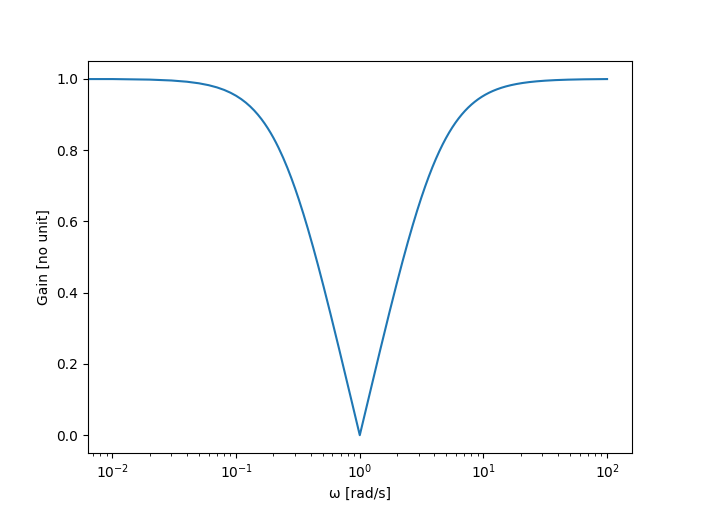
\includegraphics[width=\linewidth]{notch-resp}
  \caption{Typical Notch filter's response with $R = 10\Omega$, $C = 1 \,\textrm{Farad}(F)$ and $L = 1 \,\textrm{Henry}(H)$.}
  \label{fig:notch-resp}
\end{subfigure}
\caption{Notch filter design and its electrical response.}
\label{fig:test}
\end{figure}

This filter is commonly called a \textit{Notch filter} or \textit{band-stop filter} as its purpose is to block a certain range of frequency in the response of the circuit. The gain of such a circuit is dicted by the formula\footnote{See appendix \ref{notch_filter_formula}}:
\begin{equation}
\left\lvert \frac{V_{out}}{V_{in}} (\omega) \right\rvert = \frac{1}{\sqrt{1 + \left(\frac{R}{\omega L - \frac{1}{\omega C}}\right)^2}}
\end{equation}
where the figure \ref{fig:notch-resp} sketch a typical response of this RLC circuit. As we can see, the gain is set to 1 (i.e the output voltage has the same value than the input voltage) except for a band of frequency where the center of this gap is found to be:
\begin{equation}
\label{rlc_resonance}
\omega_0 = \frac{1}{\sqrt{LC}} \Leftrightarrow f_0 = \frac{1}{2\pi\sqrt{LC}}
\end{equation}
which is called the \textit{resonance} of the circuit caracterizing a null impedance of the LC component\footnote{Of course, it does not mean that L and C are null but \eqref{rlc_resonance} is an equivalent of removing the inductor and the capacitor from the Notch filter.}.

Moreover, the whole circuit, as depicted in figure \ref{fig:detector-fst} plus the Notch filter, has a hidden filter. Indeed, the photodiodes, when enabled and receiving light, may be theoretically replaced by an equivalent circuit between as represented in figure \ref{fig:equiv-diode}: one current source in parallele of a capacitor and a resistance.

\begin{figure}[h!]
\caption{Equivalent circuit for a photodiode.}
\centering
\includegraphics[width=0.2\textwidth]{equiv-diode}
\label{fig:equiv-diode}
\end{figure}

The two capacitors associated to those two photodiodes add with an internal capacitance of the op-amp for which the value may be found in its associated data sheet. Here, we deal with a THS4021 from Texas Instrument for the op-amp and two S5971 photodiodes from Hamamatsu\footnote{Those two diodes have a high speed response of 100MHz: far more than the expected frequency of 43MHz.}. In this configuration, those three capacitors are in parallele and the total capacitance reads:
\begin{equation}
C_{total} = C_{photodiode,1} + C_{photodiode,2} + C_{op-amp}
\end{equation}
In theory (i.e from the data sheets) we have a total capacitance of $9pF$ (pico-Farads) but in practice, and with further analyses of the dectector, it turns out that $C_{total}$ is around $14pF$. Note that this formula is clearly the same for resistors in series. Now, the figure \ref{fig:detector-sec} shows the simplified circuit of the dectector with the Notch filter and the \textit{hidden} filter, where we replaced the resistor .

\begin{figure}[h!]
\caption{Detetector's circuit design with the additional filters.}
\centering
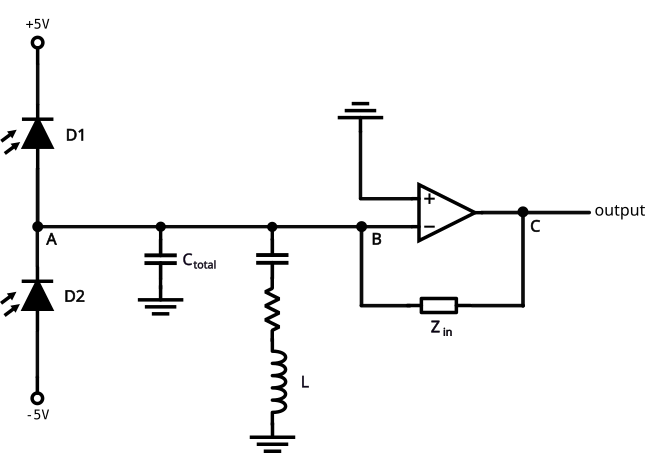
\includegraphics[width=0.7\textwidth]{detector-sec}
\label{fig:detector-sec}
\end{figure}

As we can see, this additional capacity $C_{total}$ is in parallele with the inductor $L$ of the Notch filter. This new LC component is called a \textit{tank filter} and, in contrary to its counter part LC in serie, the tank filter allows only a certain range of frequency to go through the circuit:
\begin{equation}
\left\lvert \frac{V_{out}}{V_{in}} (\omega) \right\rvert = \frac{1}{\sqrt{1 + R^2\left(\frac{1}{\omega L} - \omega C\right)^2}}
\end{equation}
where figure \ref{fig:tank} sketch a typical response of this LC circuit \ref{fig:tank}. 

\begin{figure}
\centering
\begin{subfigure}{.3\textwidth}
  \centering
  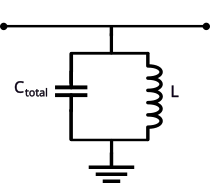
\includegraphics[width=0.8\linewidth]{tank}
  \caption{Electric circuit of the hidden tank filter: in parallel of the circuit, a capacity and an inductor in parallels.}
  \label{fig:tank}
\end{subfigure}%
\hspace{2em}%
\begin{subfigure}{.6\textwidth}
  \centering
  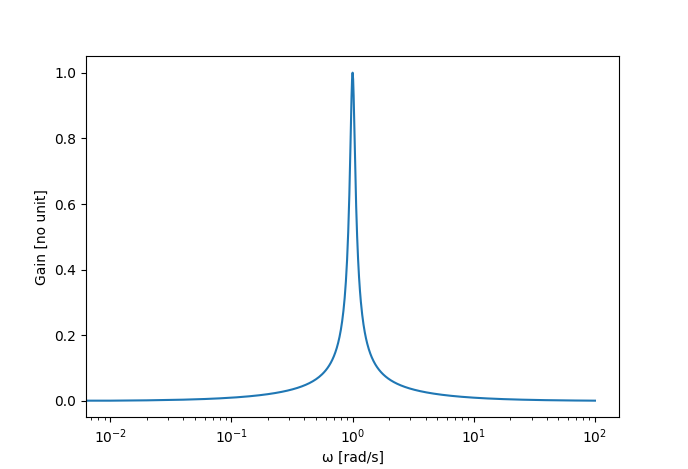
\includegraphics[width=\linewidth]{tank-response}
  \caption{Typical tank filter's response with $R = 10\Omega$, $C = 1 \,F$ and $L = 1 \,H$.}
  \label{fig:tank-response}
\end{subfigure}
\caption{Tank filter design and its electrical response.}
\end{figure}

The gain is set to 1 only for a very narrow frequency range (parametrized by the R, L and C values) which can be found to be the exact same as \eqref{rlc_resonance}: the resonance is reached when the impedance of this LC circuit is null.

As we can see, compared to the transimpedance amplifier, this circuit in figure \ref{fig:detector-sec} has an additional impedance $Z_{in}$ between the nodes (A) and (B). Considering the photodiodes as a current source, things get more complex than the transimpedance amplifier by the presence of $Z_{in}$. Actually, we use an \textit{electronic design automation software}, namely \textit{LTSpice}, in order to get the gain at the ouput of the actual detector. Then, from simulation, we get figure \ref{fig:total_gain_original} which clearly shows that the filters does not affect the interesting region which consist of a narrow bandwidth arround 43MHz: the expected signal collected from the photodiodes is amplified whereas high frequencies (i.e above 100Mhz) are removed from the output signal.

\begin{figure}[h!]
\caption{Total gain of the circuit with original components.}
\centering
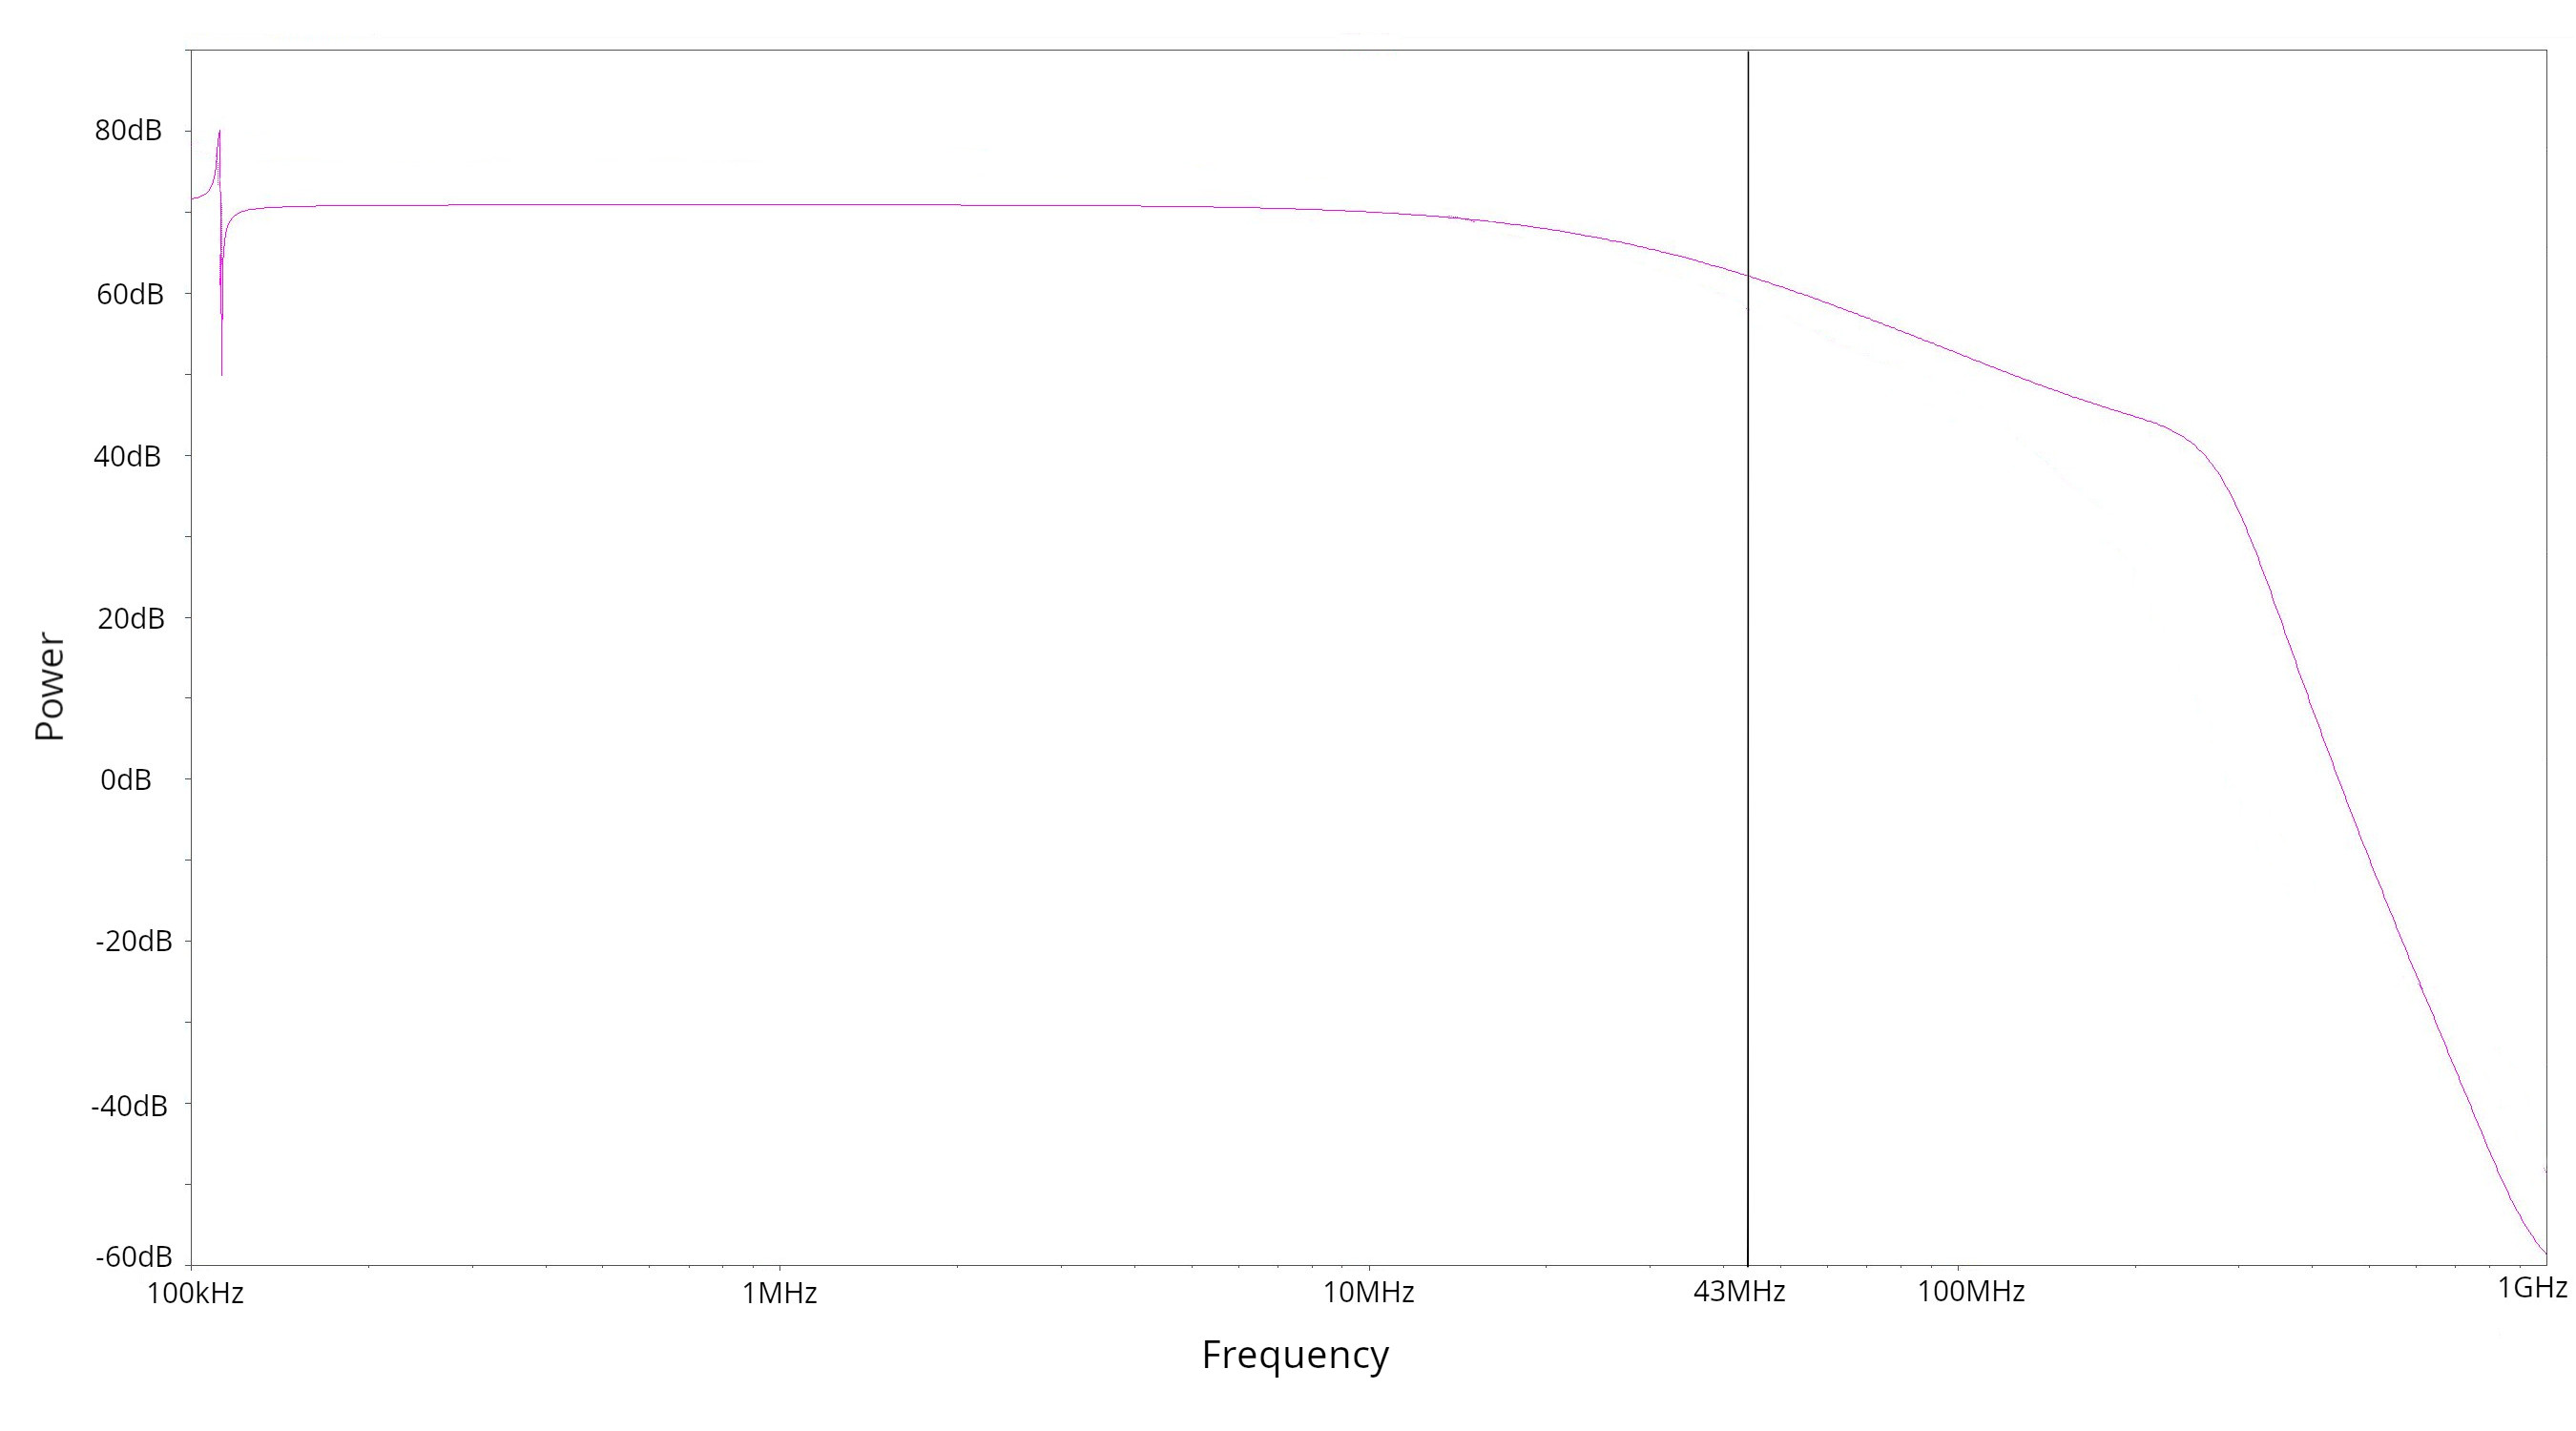
\includegraphics[width=\textwidth]{total_gain_original}
\label{fig:total_gain_original}
\end{figure}

However, we stated before that the noise is generated from the non-inverting input of the op-amp whereas the photodiodes does not receive light: the equivalent circuit corresponds to the simplified diagram which is given in figure \ref{fig:transimp}.

\begin{figure}[h!]
\caption{Basic circuit designa of a transimpedance amplifier. $V
_{in}$ is the voltage noise generated by the op-amp at its non-inverting input.}
\centering
\includegraphics[width=0.5\textwidth]{transimp}
\label{fig:transimp}
\end{figure}

This circuit is called a non-inverting voltage amplifier where the gain may be formulated as:
\begin{equation}
\textrm{Gain} = \frac{V_{out}}{V_{in}} = 1 + \frac{Z_{f}}{Z_{in}}
\end{equation}
where $Z_f$ is basically a resistor\footnote{On the real electronic scheme \ref{fig:elec-scheme}, the resistor owns an additional capacitor in parallele.} and $Z_{in}$ is composed of the filters (Notch plus Tank filter). Thanks to the inversion if the impedance, namely $1/Z_{in}$, the behavior of all the components $Z_{in}$ are inverted. In other words, the Notch filter corresponds now to a \textit{band-pass} filter whereas the Tank filter corresponds to a \textit{band-cut} filter for the electronical noise. Thereby, we need to match the band-cut filter resonance, that is to say where the gain of the electronic noise is minimum, to the main frequency of our incoming beam (i.e 43MHz).

\begin{figure}[h!]
\caption{Full electronic scheme of the actual detector. The actual component values may differ from reality as this figure has been produced for several \textit{type} of the same detector.}
\centering
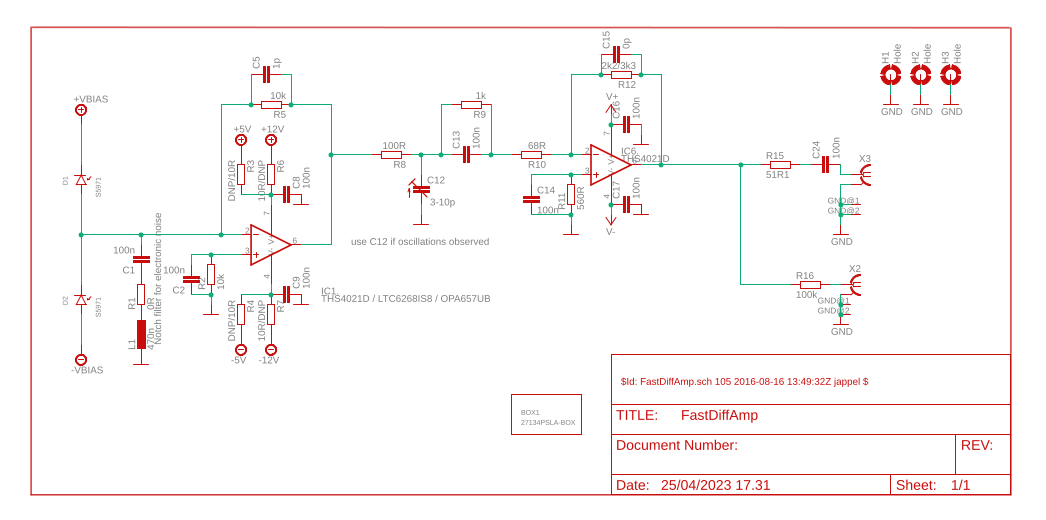
\includegraphics[width=0.95\textwidth]{elec-scheme}
\label{fig:elec-scheme}
\end{figure}

From simulation of the electronic scheme \ref{fig:elec-scheme}, we get the following gain graph \ref{fig:noise_gain_opamp_original}. 

\begin{figure}[h!]
\caption{Simulated noise gain graph with the original components.}
\centering
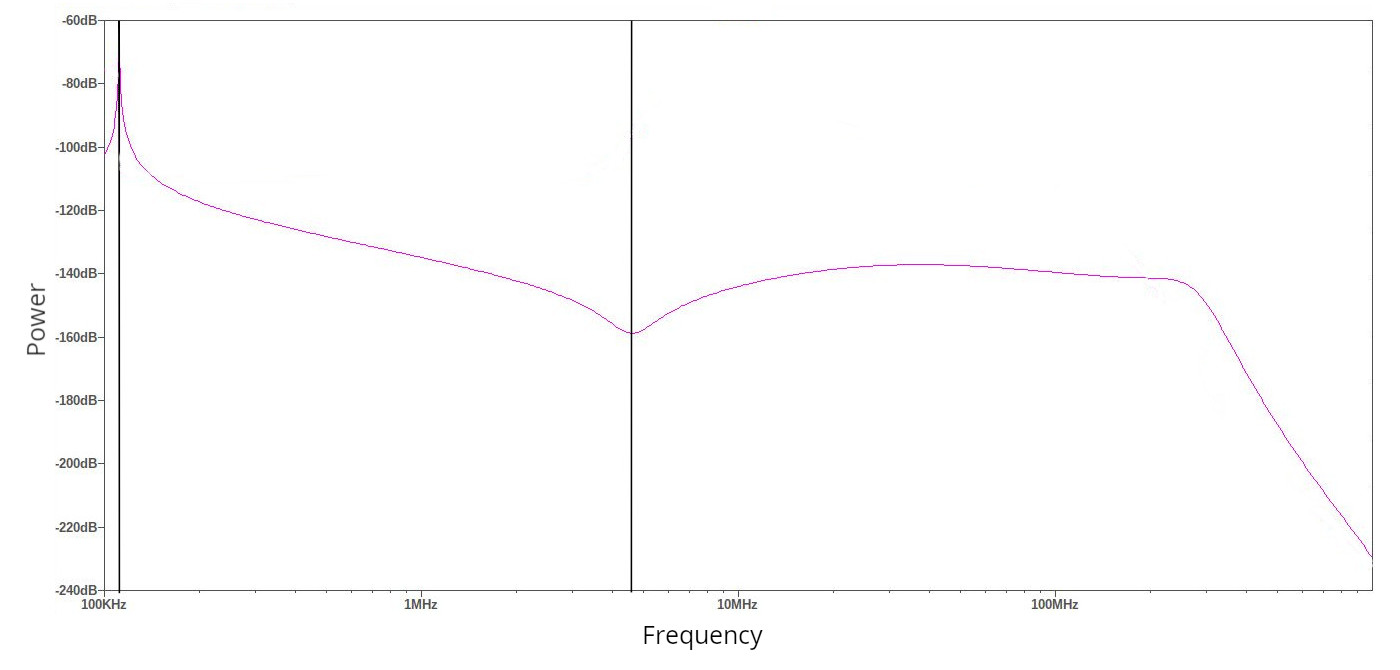
\includegraphics[width=0.8\textwidth]{noise_gain_opamp_original}
\label{fig:noise_gain_opamp_original}
\end{figure}

The peak clearly comes from the Notch filter with:
\begin{equation}
\label{peak_notch_original}
f_{notch} = \frac{1}{2\pi\sqrt{100 \times 10^{-6} \times 20 \times 10^{-9}}} \simeq 112kHz
\end{equation}
whereas the deep \textit{should} come from the Tank filter with:
\begin{equation}
f_{tank} = \frac{1}{2\pi\sqrt{100 \times 10^{-6} \times 14 \times 10^{-12}}} \simeq 4.2MHz
\end{equation}
Then, we can compare those values with the detector directly connect to the spectrum analyzer (detector under tension and photodiodes blocked from incoming light). We obtain both centered\footnote{"Centered" in a sense that the graph are localized around the interesting features.} experimental graphs \ref{fig:exp_spec_o}.

\begin{figure}[h!]
\centering
\begin{subfigure}{.45\textwidth}
  \centering
  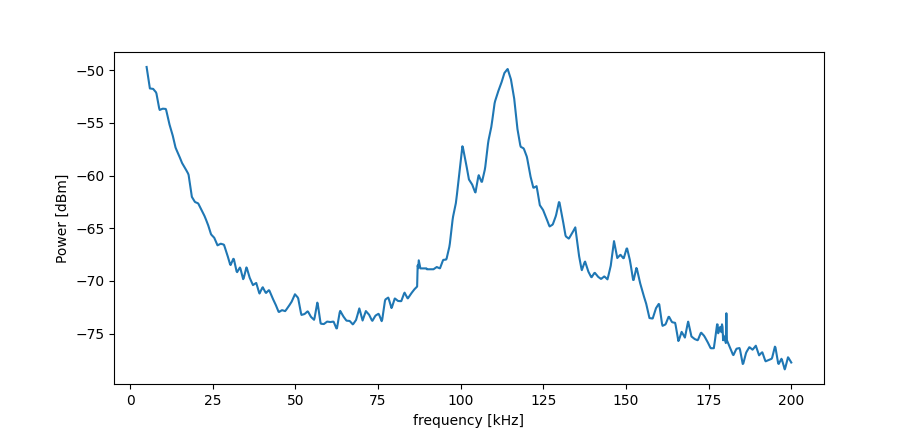
\includegraphics[width=1.1\linewidth]{opick}
  \caption{Op-amp's noise for the notch filter.}
  \label{fig:opeak}
\end{subfigure}%
\hspace{1em}%
\begin{subfigure}{.45\textwidth}
  \centering
  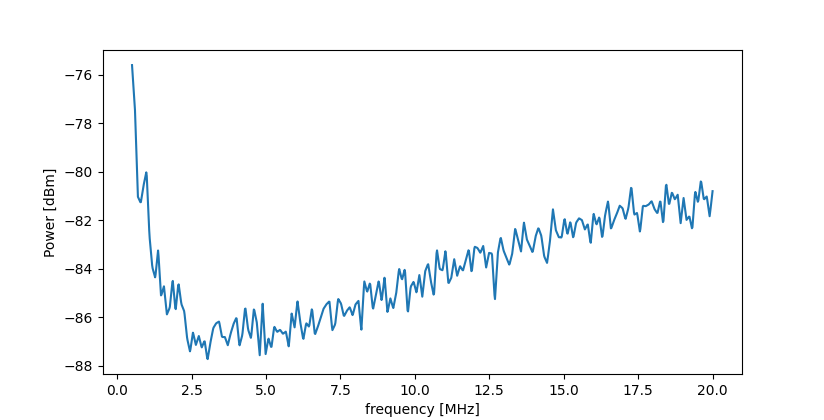
\includegraphics[width=1.1\linewidth]{odeep}
  \caption{Op-amp's noise for the tank filter.}
  \label{fig:odeep}
\end{subfigure}
\caption{Experimental spectrums with the original components.}
\label{fig:exp_spec_o}
\end{figure}

The peak corresponds very well to the theoretical one \eqref{peak_notch_original} with an error of about $\pm1$kHz. However, the deep is clearly shifted to $-400$kHz (i.e located at $3.8$MHz) on the \textit{simulation} graph \ref{fig:odeep}, and is even shifted to $-700$kHz (i.e located at $3.5$MHz) on the epxerimental graph: it appears after further tests and modificatiosn that there is a lack of understanding in the capacitor value and the best guess would be that the surrounding of the circuit induces a non-linear behavior\footnote{\textit{Non-linear} meaning that this difference has a tendency to increases while the resonances increase (i.e when modifiying the components).} of the stray capacitance of $14pF$, thus explaining the shift with the experimental graphs.\footnote{Note the difference of absolute power on the y-axis between the experimental and simulated noise spectrums: that is due to the parameters entered in LTSpice which artificially decreases the \textit{zero} level. That is why, the unit of the y-axis for the simulated figures are in dB and not in dBm.}

Nevertheless, it is obvious that the drop of electronic noise is not localized on the right spot: ideally, the minimum noise gain would be at $43$MHz. In that way, we modify the inductor value to a theoretical one, namely $0.82\mu F$ instead of $100\mu F$:
\begin{equation}
f_{tank} = \frac{1}{2\pi\sqrt{0.82 \times 10^{-6} \times 14 \times 10^{-12}}} \simeq 46MHz
\end{equation}
which appears to be $3$MHz out of resonance. However, when simulating the full circuit with this new value for the inductor, one obtains the graph \ref{fig:noise_gain_opamp_new}.
\begin{figure}[h!]
\caption{Simulated noise gain graph with the new inductor.}
\centering
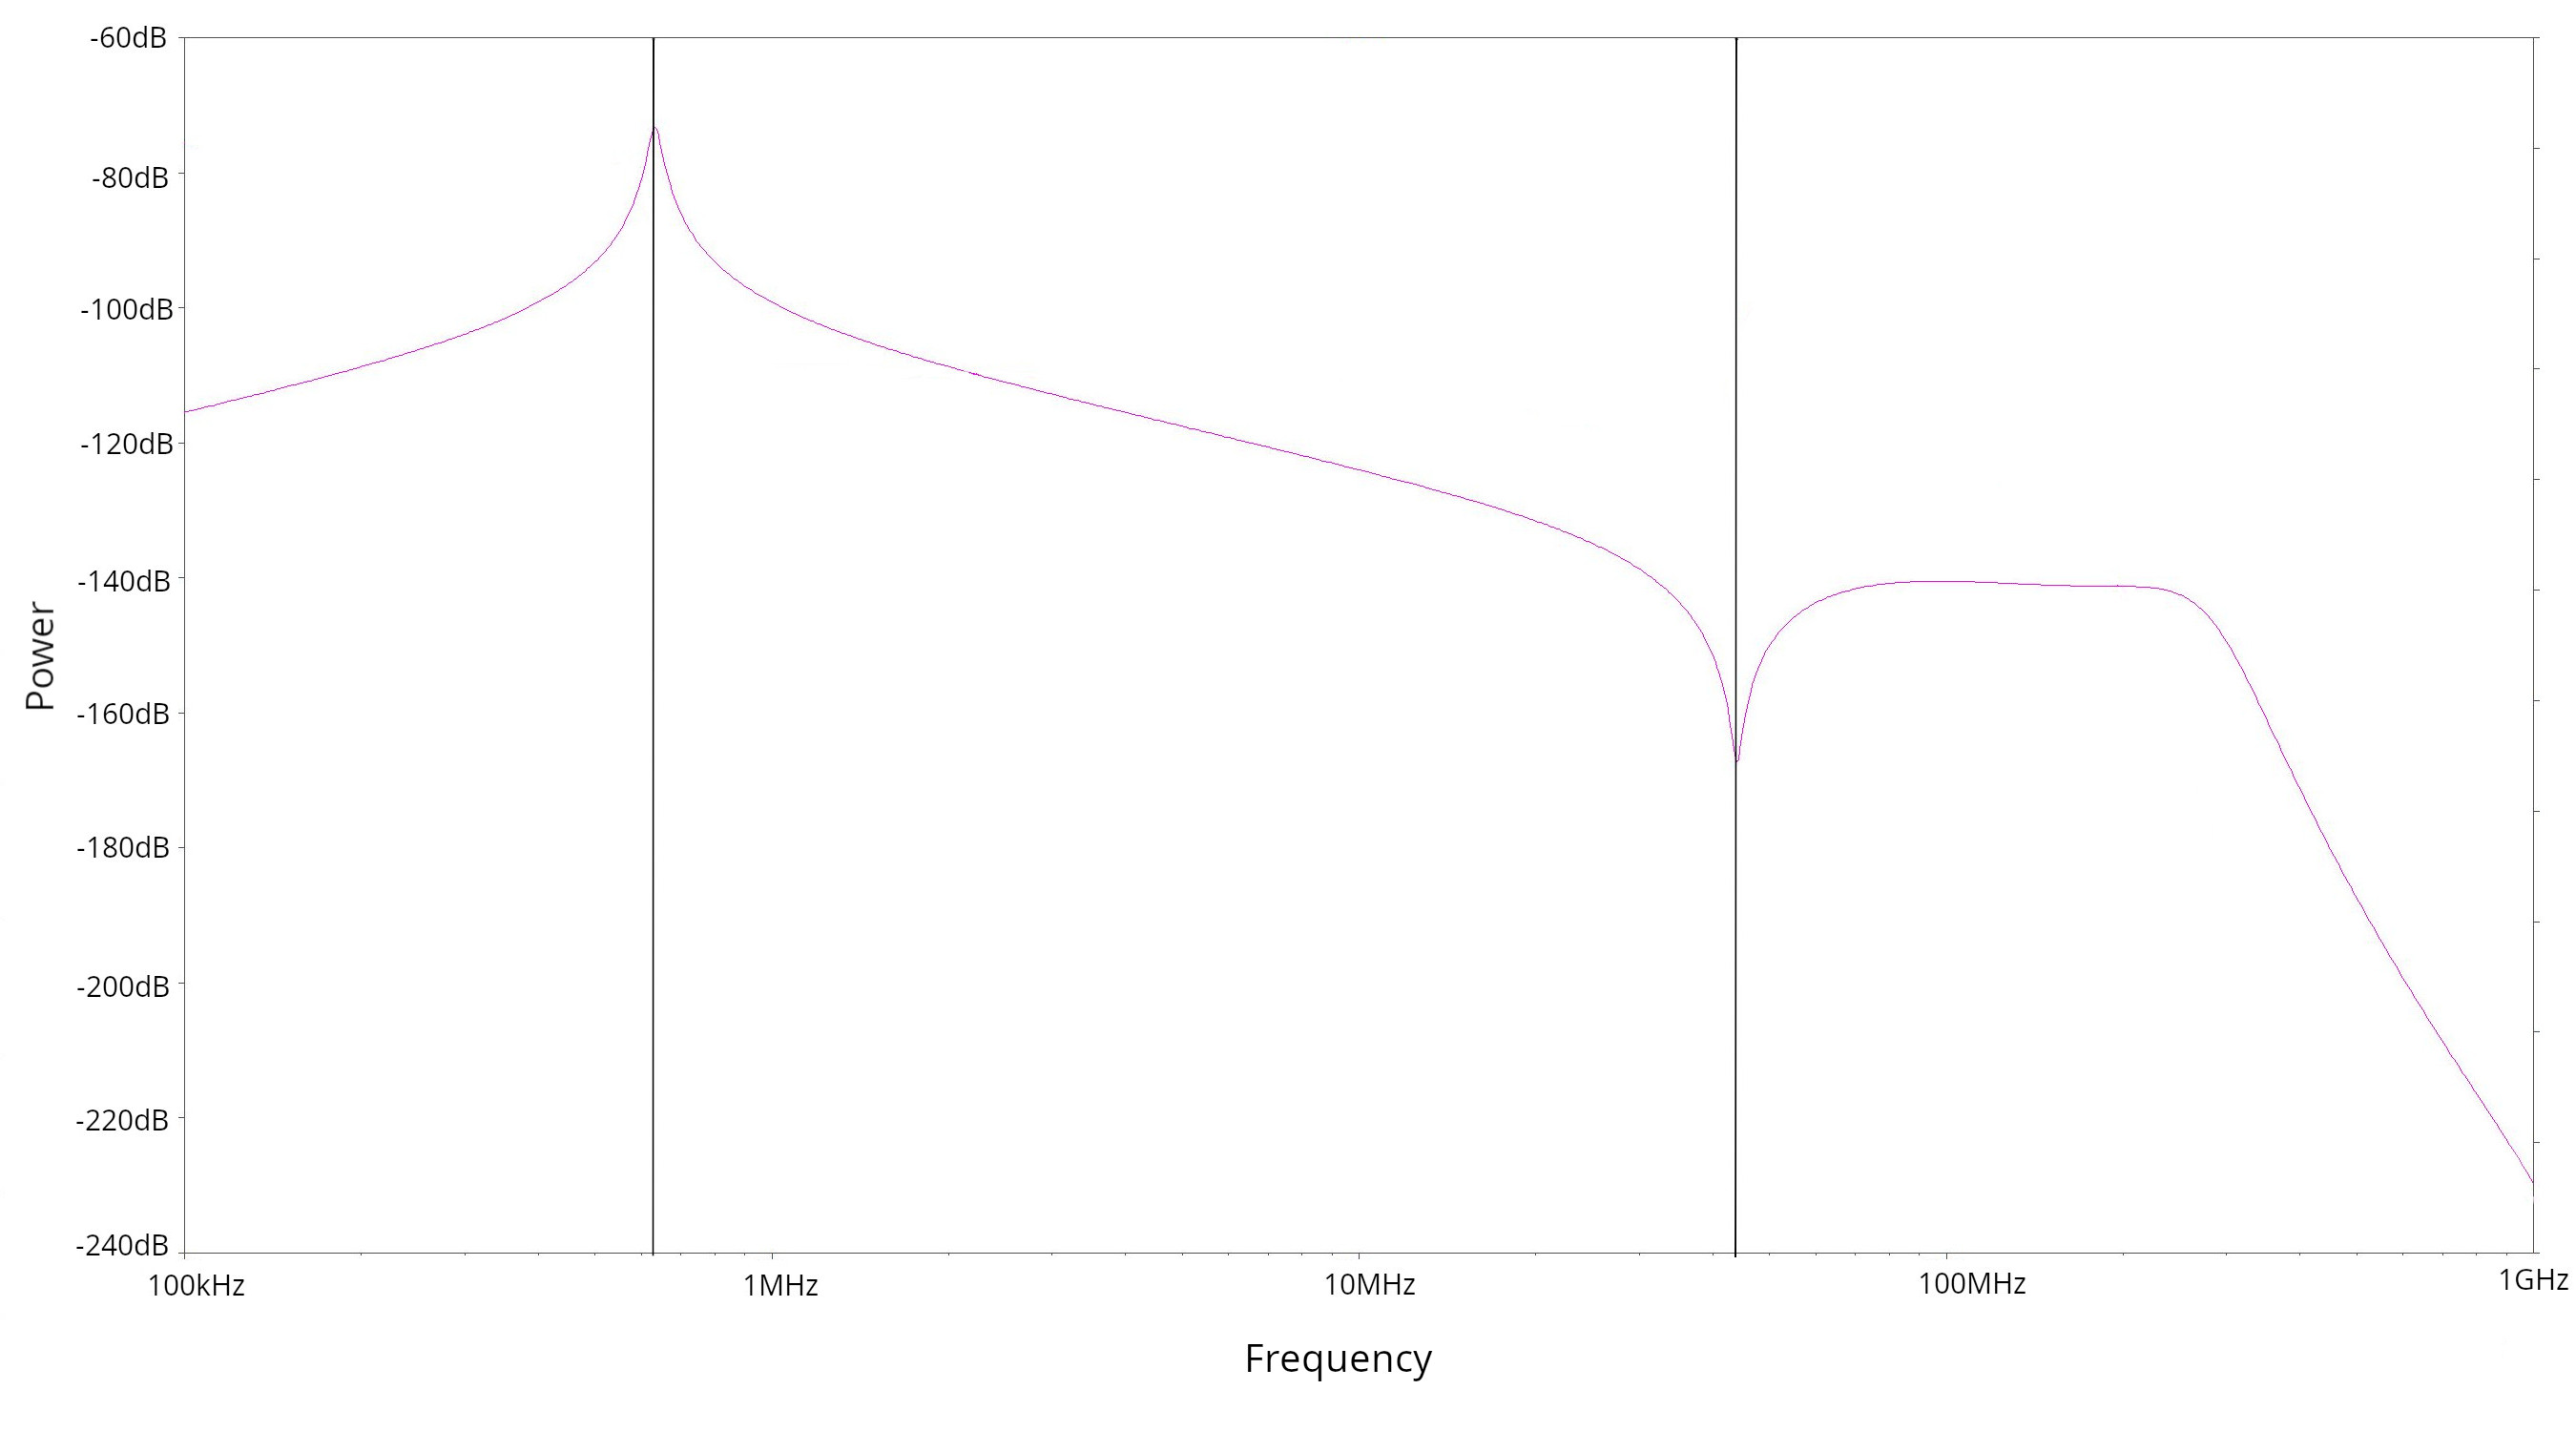
\includegraphics[width=\textwidth]{noise_gain_opamp_new}
\label{fig:noise_gain_opamp_new}
\end{figure} The deep of $-170$dB clearly corresponds to the $43$MHz resonance. Thus, modifying the inductor to $0.82\mu F$ should move the deep to the correct position of $43$Mhz. Moreover, in the worst case of misunderstanding this misalignment with the theoretical resonances, the inductor would change values from several hundreds of micro-Farads, in order to reach a theoretical maximum of $60$MHz: for example, taking $L=0.5\mu F$ would give approximately $60$Mhz of resonance for the deep and considering a shift to the left, we should attain the targeted deep of $43$MHz. In that way, we commanded several inductors of values ranging $100nF$ to $2\mu F$ and replace the orginal inductor by removing and making a new soldered joint.

Picture of the detector

At the end of the day, we have an inductor of exactly $0.8\mu F$ which allow a nice deep of the noise gain of roughly $-85$dBm.

\begin{figure}[h!]
\centering
\begin{subfigure}{.45\textwidth}
  \centering
  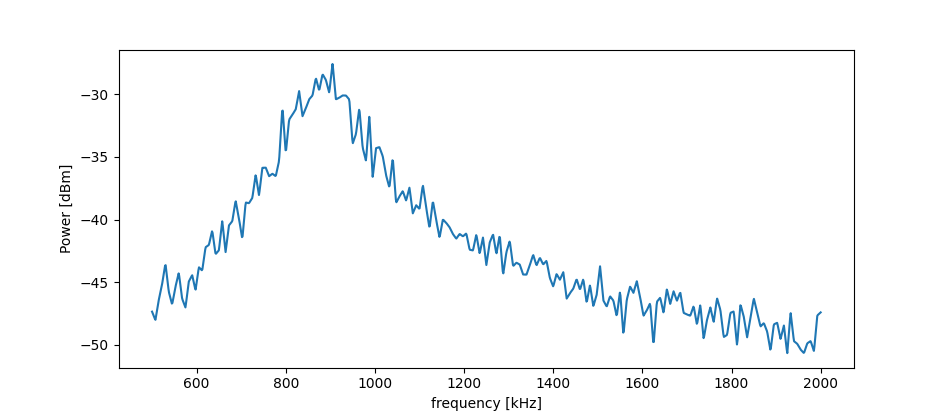
\includegraphics[width=1.1\linewidth]{mpick}
  \caption{Op-amp's noise for the notch filter.}
  \label{fig:mpeak}
\end{subfigure}%
\hspace{1em}%
\begin{subfigure}{.45\textwidth}
  \centering
  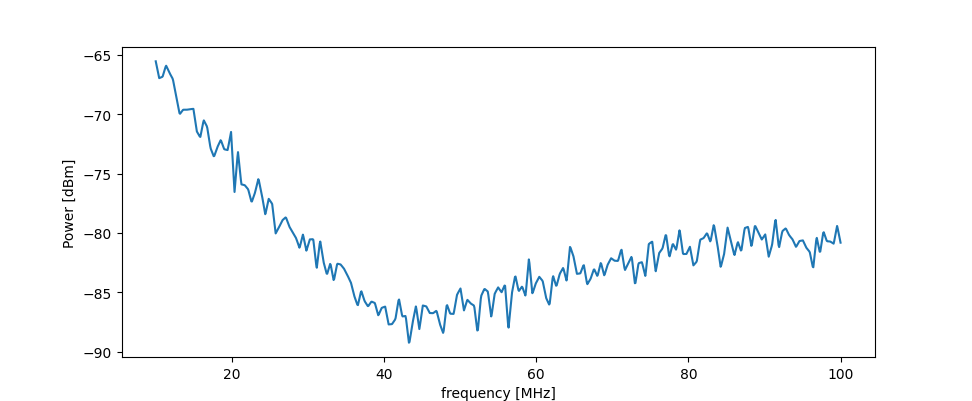
\includegraphics[width=1.1\linewidth]{mdeep}
  \caption{Op-amp's noise for the tank filter.}
  \label{fig:mdeep}
\end{subfigure}
\caption{Experimental spectrums with the new inductor.}
\label{fig:exp_spec_m}
\end{figure}

The graph \textit{fig:mpeak} also shows the peak from the Notch filter which, by virtue of \eqref{rlc_resonance} moved to the right at, approximately, $900$kHz where, from simulation, we were excpecting it at $700$kHz. However, the deep on graph \ref{fig:mdeep} is very well localized around the expected light frequency of $43$Mhz.

Moreover, the new total gain graph \ref{fig:total_gain_new} clearly shows that the ouput voltage is not affected by the filters.

Finally, we succeded to modify the detector with our frequency requirements by replacing some components of the filters, in order to reduce as much as possible the electrical noise comming from the active components, namely the op-amp.

The next sections will focus on the parametrization/configuration of the detector which involves, among others, saturation test, amplification noise test and technical procedures in order to make sure that the experiment works in the parameter's range of the detector.

\begin{figure}[h!]
\caption{Total gain of the circuit with the new inductor.}
\centering
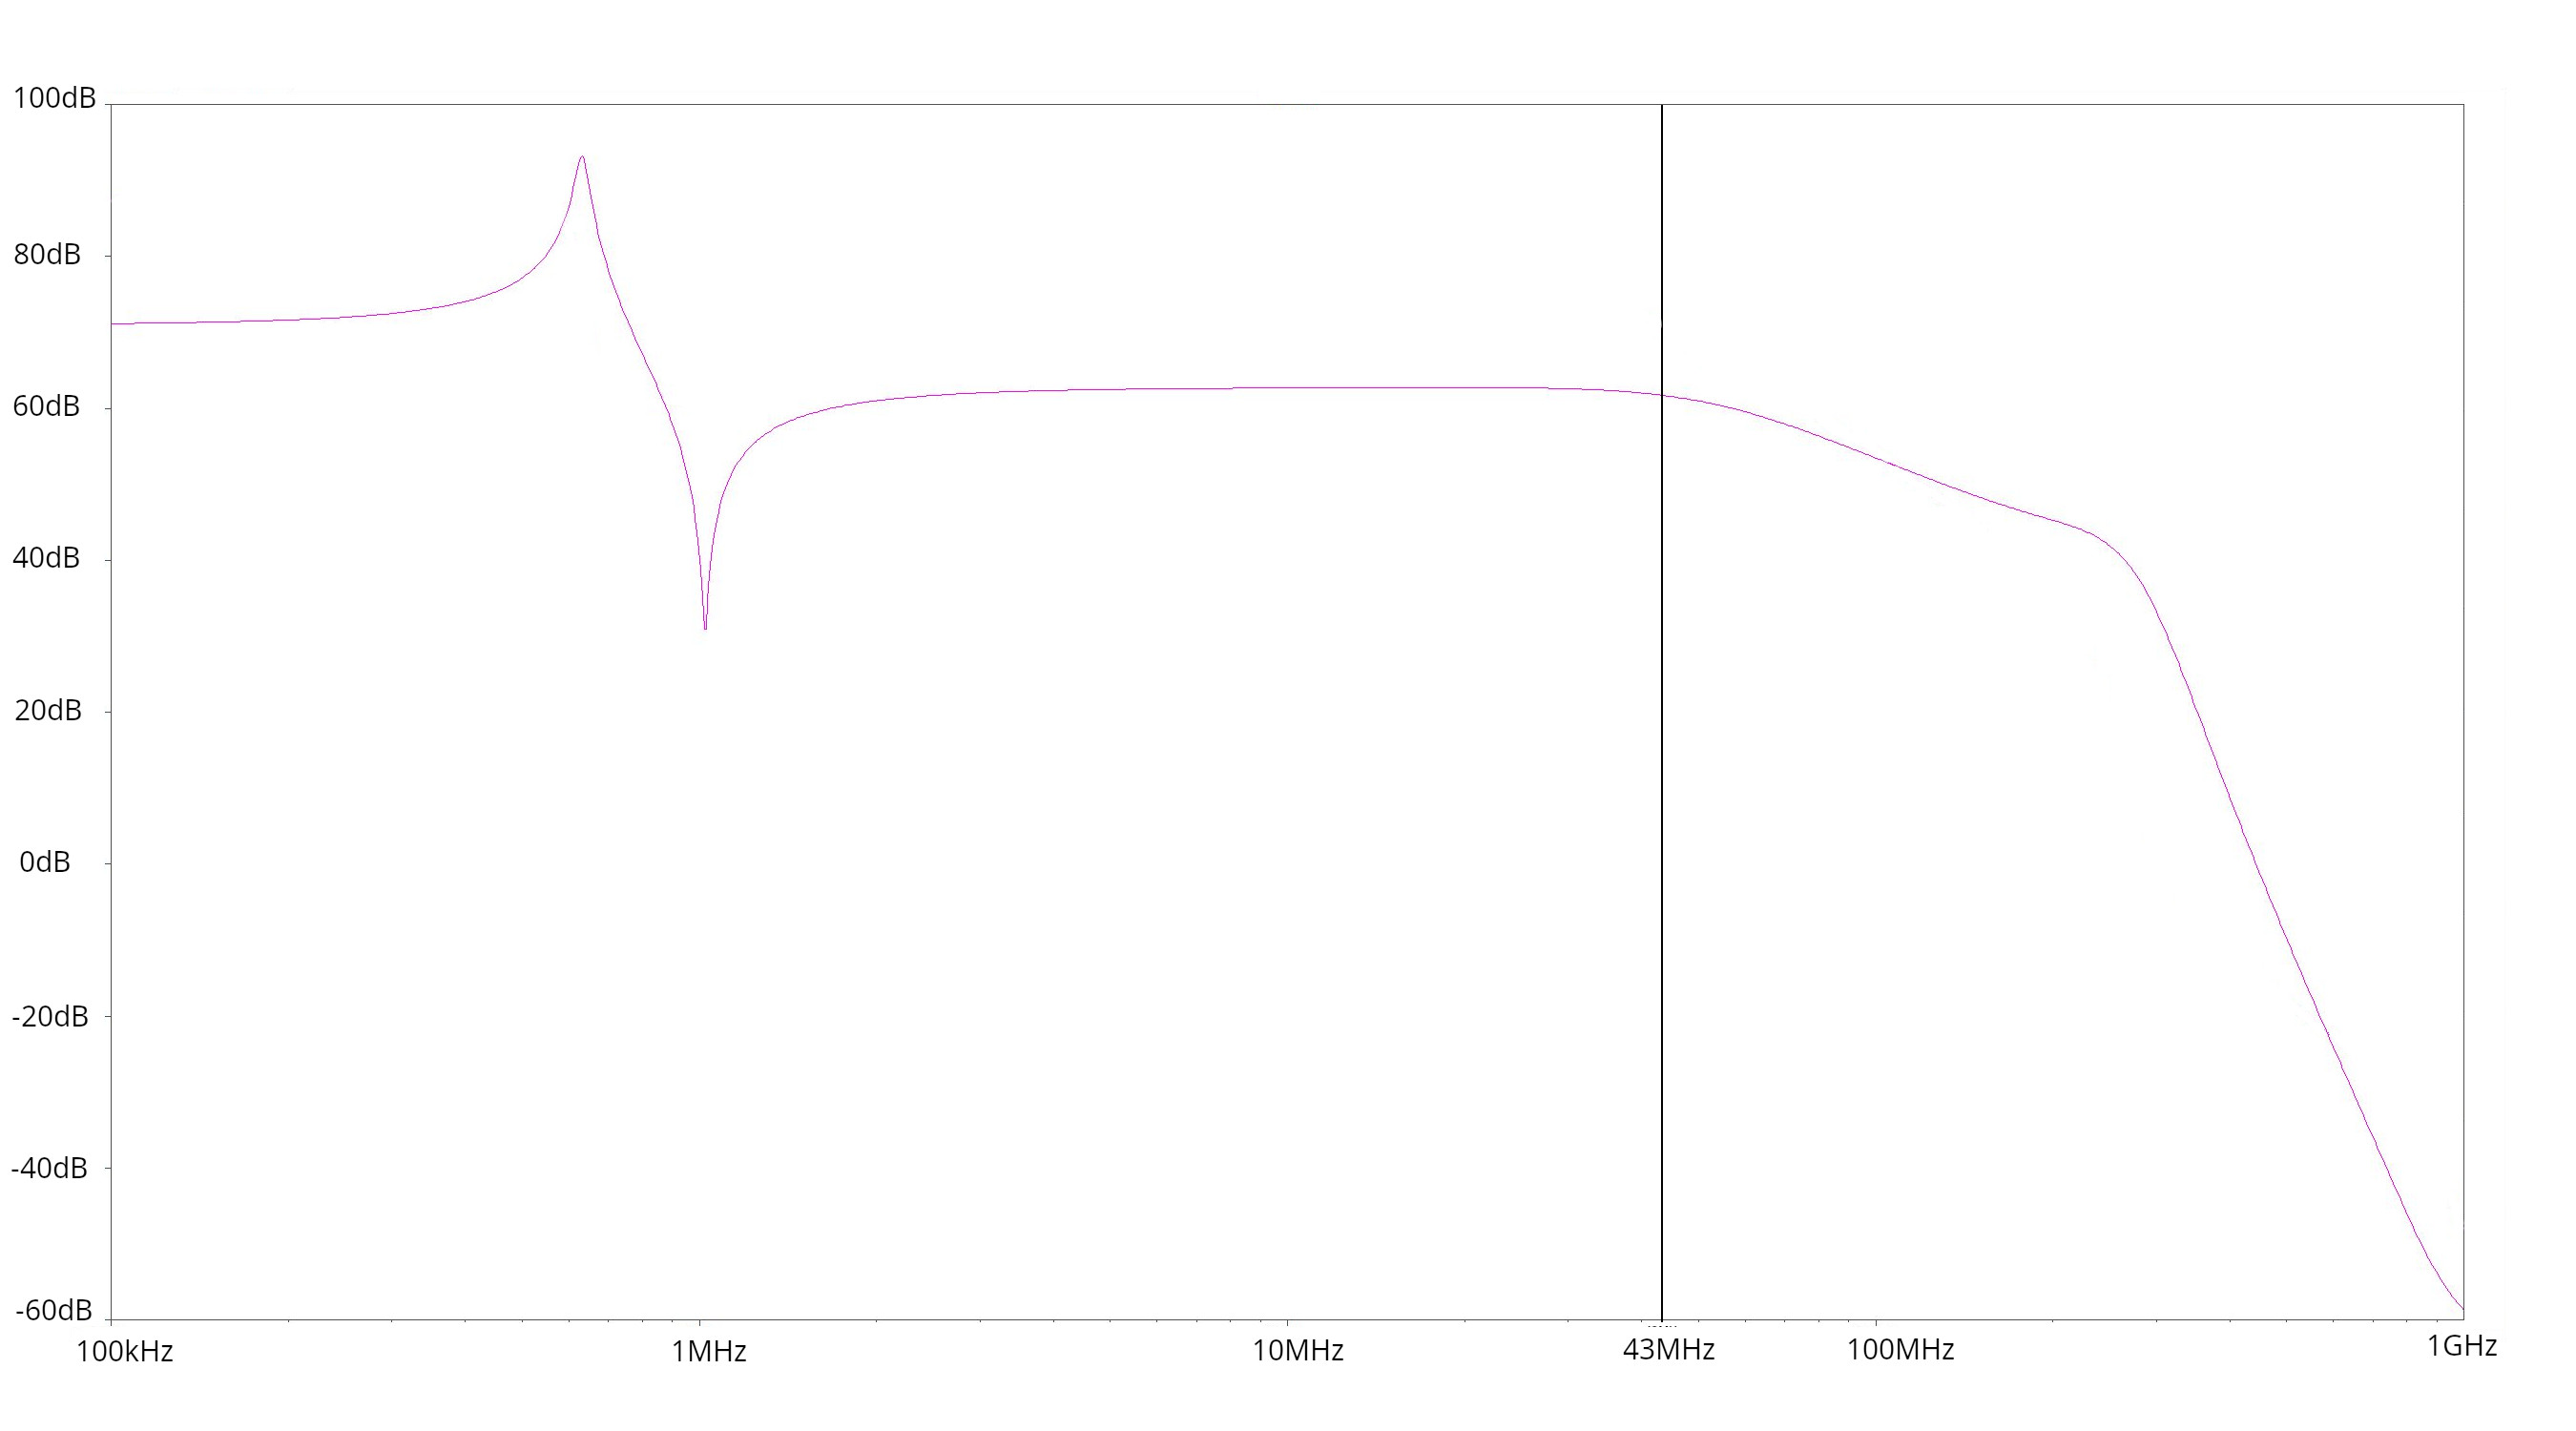
\includegraphics[width=\textwidth]{total_gain_new}
\label{fig:total_gain_new}
\end{figure}

\section{Diode's size versus laser's cross section area}

Firstly, we start to simply verify if the \textit{final} laser beam, which is composed of the cavity beam plus the optical oscillator laser, is not oversized compared to the diode area. Inddeed, the specification sheet for those diodes (S5971) gives an explicit photosensitive diameter size of 1.2mm (the sheet specifies it as the \textit{area size}). In other words, the laser beam after the overlap of the beam splitter must have a diameter of less than 1.2mm. Otherwise, we would \textit{spatially saturate} the diodes and lose some part of the laser's cross section area.

Therefore, we add two lenses with a focal length of 50mm each in front of both diodes. We place them at 65mm from the diodes respectively. From a geometrical optic's point of view, the laser is essentially an ensemble of parallel lines of light as one could perceive from a distant star. Thereby, from the optical rule involved for a convergent lens, the laser's parallel lines firstly converge after crossing the lens until they all reach the focal point, then diverges. With this configuration, summarized in figure \ref{fig:heterodyne-lens}, the diodes are exactly 15mm after the focal point of the lenses. 

\begin{figure}[h!]
\caption{Heterodyne experiment with lens added.}
\centering
\includegraphics[width=0.8\textwidth]{heterodyne-lens}
\label{fig:heterodyne-lens}
\end{figure}

As the focal point to diode distance is lower than the focal length, the resulting laser's cross section area while hitting the diodes is smaller than the original one (i.e before the lens). This ratio is computed as follow:
\begin{equation}
\label{lens_cross_section_ratio}
\textrm{Cross Section Area Ratio} \stackrel{\text{def}}{=} r_{cs} = \frac{\vert d-f \vert}{f}
\end{equation}
where $d$ is the the focal point to diode distance whereas $f$ is the focal length. Note the absolute value which avoid the ratio \eqref{lens_cross_section_ratio} to become negative if $d$ is smaller than $f$ (i.e the diodes reside in the \textit{convergent} part of the lens). Thus, we obtain in our case a $r_{cs} = 0.3$. In other words, the beams hitting the diodes after crossing the lenses are apprxoimately three times smaller in area than the original beam.

In order to check if the amount $r_{cs} = 0.3$ of cross section area reduction is sufficient, we shall move progressively the dectector perperdicularly to the optical axis. As represented in figure \ref{fig:heterodyne-lens}, we block one diode while transposing lateraly the detector and recording the DC output voltage\footnote{The DC component of the electric signal, when only one diode is enabled, is proportional to the intensity received (until saturation) independently of the frequencies of the light. }.

According to the laser beal size compared to the photosensitive area, two cases are distinguishable:
\begin{itemize}
	\item The laser beam size is smaller than the photodiodes. The voltage output increases, reach a plateau of constant voltage ouput, then decreases.
	\begin{figure}[h!]
	\centering
	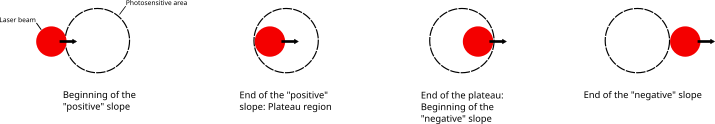
\includegraphics[width=0.9\textwidth]{diode-size-sm}
	\label{fig:diode-size-sm}
	\end{figure}
	\item The laser beam size is equivalent to the photodiodes: Fig ??. The voltage output increases, reach a maximal peak of voltage, then decreases.
	\begin{figure}[h!]
	\centering
	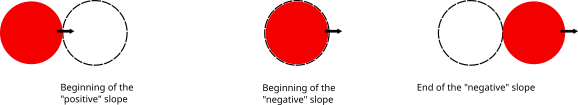
\includegraphics[width=0.7\textwidth]{diode-size-eq}
	\label{fig:diode-size-eq}
	\end{figure}
	\item The laser beam size is bigger than the photodiodes: Fig ??. The voltage output increases, reach a plateau of constant voltage ouput, then decreases.
	\begin{figure}[h!]
	\centering
	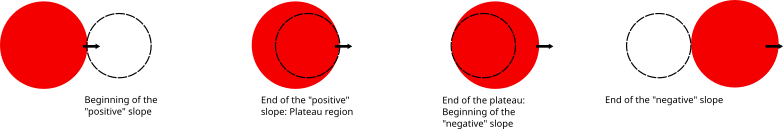
\includegraphics[width=\textwidth]{diode-size-big}
	\label{fig:diode-size-big}
	\end{figure}
\end{itemize}
As we can notice, this technic shows the same behavior for bigger or smaller beam sizes. However, it is possible to evaluate the beam's diameter by measuring the distance between the beginning and the end of the slope. Indeed, this measure is literraly the position when the laser's beam starts hitting the photosensitive area (i.e this is the beginning of the slope) whereas when the laser's beam is fully included into the photodiode (i.e this is the \textit{plateau} and the end of the slope). Moreover, if the beam is bigger than the photosensitive area, the plateau (thus the end of the slope) will be reached when the beam covers entirely the photodiode: the \textit{slope distance} is the photodiode's diameter, not the beam's diameter. In other worlds, if we measure less than 1.2mm for the \textit{slope distance} then the laser's beam is encompassed into the photosensitive area.

Figure \ref{fig:diode-size-plot} shows the results for two different powers involved in the local oscillator: using two powers ensure that we are not saturating the photodiodes in term of intensity when measuring the beam's size. As we consider the cavity laser very weak (in order of picowatts), the main power come out of the reference laser\footnote{In that case, we use two very distinct powers which are tuned mechanically, with a button on the \textit{laser box}. This is not a \textit{clean} method because it is not very precise and we shall use a different method in the next section.}.

\begin{figure}[h!]
\caption{Average voltage ouput of the detector according to the relative position of one of the diode (The other diode is blocked from light), for two different power of the local oscillator.}
\centering
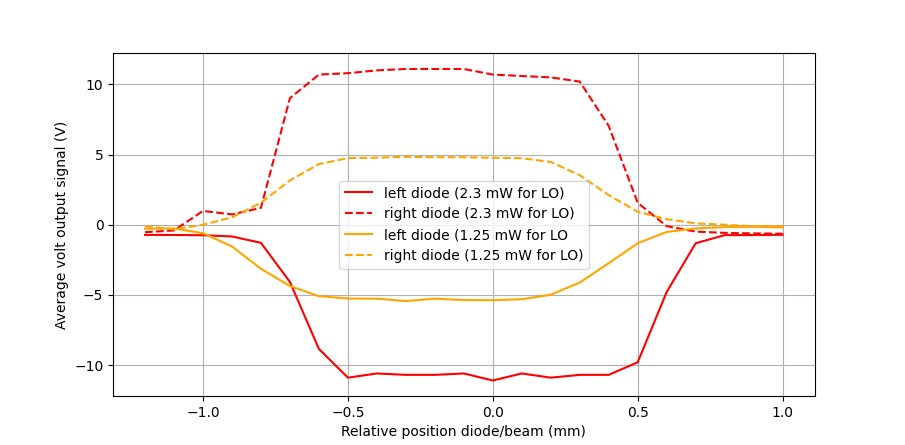
\includegraphics[width=\textwidth]{diode-size-plot}
\label{fig:diode-size-plot}
\end{figure}

The yellow curves (low power) may be considered not saturating the diodes as those curves doesn't reach the same maximum than the red curves (high power).\footnote{Note than this argument, alone, does not allow to decide if the red curves means the saturation of the diodes or not.}. We can measure the beam's diameter as roughly 0.6mm for the red curves and 1mm for the yellow curves. Thus, the laser beam is well encompassed into the photodiodes. Secondly, those measurements mean that the power associated to the read curves are saturating the diodes: before the beam hits entirely the photosensitive area, the detector reaches its maximum/minimum of output voltage which is now determined to be $\pm11$ volts.

Note that the whole procedure relies on the horizontale diplacement. Naively, one could repeat the process accross different vertical positions: one should obtain a 2D map of the output voltage according to the relative beam to diode position. Nevertheless, we only check in practice that the ouput voltage cannot be maximized while moving the dectector up or down when the beam reaches the plateau region (This is done with the yellow curves power, knowing that we are not already saturating the diodes).

\section{Power to noise ratio}

As we already mentioned in section 2.2 (Balanced heterodyne setup), the detection of light involves an amplification of the light's noise dependenging on the light's power. The photocurrent $i(t)$ produced by the diodes may \textit{always} be written with the sum of the mean photocurrent and a shift to the mean:
\begin{equation}
\label{i_split_delta_i}
i(t) = \left\langle i \right\rangle + \Delta i(t)
\end{equation}
where the mean is obviously a constant over time. By definition of $\Delta i(t)$, its variance is not null. As the electrical power is given by the well known formula $P = U \times I$, applying \eqref{ueqri} gives naturally the noise power definition:
\begin{equation}
\label{def_p_noise}
P_{noise}(t) \stackrel{\text{def}}{=} R \times (\Delta i(t))^2 
\end{equation}
where $R$ is a dummy constant dependent on the circuit design, meaning that the noise power is proportional to the variance of the photocurrent. However, the choice $R$ is not innocent: it is the \textit{resistance/impedance load} of the circuit, namely $Z_f$ from a previous section, which transforms the current into a voltage. The current-voltage link also implies that the noise power can be equivalently defined through the voltage's variance. At this stage of the development, we do not make any assumption on the source of the variance (i.e noise) of the current: this variance may come from the quantum noise and/or the photodiode noise which may produce some \textit{randmoness} from the transformation \textit{intensity to photocurrent}\footnote{We consider the photocurrent \textit{after} the diodes but \textit{before} the transimpedance amplifier: no electrical noise yet.}.

It can be shown\footnote{See Fox ??} that the variance of the photocurrent from an incoming light is proportional to its mean value (with certain conditions on the statistics of the light, namely, having a \textit{classical} light):
\begin{equation}
\label{delta_i_var_prop_i}
(\Delta i(t))^2 \propto \left\langle i \right\rangle
\end{equation}
This relation explicitely says that the quantum noise of a classical light (i.e with a Poissonian distribution) is proportional to the mean photon number. Then, putting \eqref{delta_i_var_prop_i} into \eqref{def_p_noise} gives:
\begin{equation}
\label{p_noise_i_mean}
P_{noise} \propto \left\langle i \right\rangle
\end{equation}
where $P_{noise}$ is not dependent on time anymore if we consider the mean current as constant over time\footnote{The noise power is not dependent on the frequency of the photocurrent either: that is why it is called \textit{white noise}.}. Then, we consider the photocurrent as proportional to the light intensity hitting the diodes (i.e no randomness into the photodiodes). Thus it comes\footnote{Formally we define the light intensity by its Poynting vector which is in watt per meter-squared. However, the measured power (i.e experimental) is in watts, thus normalized to the beam's cross section area.}:
\begin{equation}
\textrm{Noise power (in watts)} \propto \textrm{Light intensity (in watts)}
\end{equation}
In other words, increasing the intensity of the incoming light also increases linearly the variance of the photocurrent, that is to say, the quantum noise.

As we collect the ouput voltage \textit{after} the whole circuit, the electrical noise is superposed to the quantum noise: as those two are uncorrelated, they add together. This means that the noise value, or equivalently the variance of the photocurrent, when no light hits the diodes, is exactly the amount of electrical noise in the circuit. Then, adding light progressively gives a linear curve which is the power to noise ratio. Obviously, this curve is limited by the saturation of the circuit\footnote{The global saturation could also be induced by the saturation of the photodiodes but it turns out experimentally that the saturation is made by the electrical components first, which cannot support a too high current/voltage level.}.

In order to check experimentally this behavior and evaluate the power to noise ratio, we need a precise and efficient method to tune the local oscillator's power. To do so, we use a pair of optical devices:
\begin{itemize}
	\item A polarizer: this device allows only light with the same polarization to cross it. For a linearly polarized electric field, things get mathematically simpler as the resulting field $\vv{E}_{out}$ is the equivalent of the entering field $\vv{E}_{in}$ projected along the polarizer's unitary vector $\vv{e}_{pol}$:
	\begin{equation}
	\vv{E}_{out} = \left( \vv{E}_{in} \cdot \vv{e}_{pol} \right) \vv{e}_{pol}
	\end{equation}
	\item A waveplate: here we use a \textit{lambda-half} waveplate (abbreviated $\lambda/2$-waveplate) and for a linearly polarized electric field, this device simply rotates the polarization's direction of the electric field.  
\end{itemize}

Assuming that the input electric field is linearly polarized (which is the case experimentally), coupling those two devices makes a very precise power-tunable instrument. Figure \ref{fig:wp-pol-setup} represents how they must be placed along the optical axis.

\begin{figure}[h!]
\caption{Waveplate and polarizer setup as a power-tunable instrument. Note that the incoming beam doesn't to be necessary vertically polarized. Only the relative angle between the waveplate and polarizer is relevant for amplitude reduction}
\centering
\includegraphics[width=0.9\textwidth]{wp-pol-setup}
\label{fig:wp-pol-setup}
\end{figure}

The waveplate rotate the electric field and the polarizer project the electric field: if the E-field is parallel to the polarizer axis after the waveplate, the output amplitude is the same as the input one. If the E-field is perpendicular to the polarizer axis after the waveplate, the ouput amplitude is null. Every polarisation's direction of the E-field in between shall give a reduced amplitude compared to the maximum amplitude: because of the scalar operation, the amplitude relation is not linear but \textit{cosine} dependent, hence very sensitive for almost perpendicular E-fields. The ensemble of Fig \ref{fig:wp-pol-setup} is placed before the beam splitter along the local oscillator's optical axis as in Fig \ref{fig:heterodyne-wp}.

\begin{figure}[h!]
\caption{Complete setup with the group Waveplate\&Polarizer added.}
\centering
\includegraphics[width=0.8\textwidth]{heterodyne-wp}
\label{fig:heterodyne-wp}
\end{figure}

As stated in section 2.2 (Balanced heterodyne setup), the resulting amplitude of the overlapping of two linearly polarized E-field is maximized when they are parallels. In this way, we have to ensure that the field coming from the cavity (i.e the superradiant laser) is collinear to the local oscillator without involving the waveplate into the setup. In practice, the cavity field is maintained as vertically polarized\footnote{For other experiences in the lab, the polarization of the cavity field is considered as vertical, thus always checked as vertical before starting any experiment.} and we align the polarizer along the same axis. By looking at the spectrum analyzer, the peak at 43MHz shall vary between zero and a maximum while rotating the main axis of the polarizer: zero means perpendicular polarization whereas the maximum means parallel/collinear polarization. It is important to notice that when reaching perpendicular polarization, the measured total beam power is not null but only the terms \eqref{mix_hetero_ic} and \eqref{mix_hetero_id}, hence the 43Mhz beat (i.e the $\delta\omega$) vanishes.

Once the fields are collinear, it suffices to put the waveplate into the setup and rotate it: this involves a rotation of the local oscillator's E-field, hence a power variation of the resulting beam (i.e after the polarizer).

Now, the principle is to calculate the variance of the recorded output voltage, according to the incoming light power (tuned by the waveplate). However, as we transfer directly the detector's signal to the oscilloscope, we face two problems:
\begin{itemize}
	\item The variance (i.e the noise) is modulated by the 43MHz signal as depicted by figure \ref{fig:beatnoise}.
	
	\begin{figure}[h!]
	\caption{Example of modulation of a perfect one-mode signal of 43MHz with a noisy signal. The resulting signal does not exhibit simply the variance of both original signals. Indeed, a demodulation process is required in order to retrieve the variance of the noisy signal independently.}
	\centering
	\includegraphics[width=0.8\textwidth]{beatnoise}
	\label{fig:beatnoise}
	\end{figure}
	
	However, the variance of a sine wave times a white noise function is not simply the variance of a sine wave (which is simply $1/2$ if the amplitude is $1$) plus/multiplied by the variance of the white noise.
	\item The received signal comprises also other frequencies than the interesting $\delta\omega/(2\pi) = 43$MHz. Hence, the rough computed variance of the output signal shall be a \textit{mix} of all the noisy signals generated by the electriccal noise, especially outside of the low-noise bandwidth of the detector. Indeed, we configured the detector to create less noise than the quantum noise only inside a narrow bandwidth around 43MHz. Everywhere else is susceptible to have high electrical noise level.
\end{itemize}

In order to rectify those issues, we shall add a \textit{demodulation} block between the output gate of the detector and the oscilloscope as represented in figure \ref{fig:wavemixer}. The idea is to mix the ouput signal with a well behaved electric sine wave called \textit{reference}: this operation is called a \textit{modulation}. At first order\footnote{The mathematical description of a wave mixer is slightly more complex. However, all the other harmonics are far beyond the highest and lowest frequencies considered at \textit{first order}, hence negligeable for our purpose.}, the wave mixer essentially creates the same components than \eqref{list_comp_light_mix} when one mixes two light beams, except the \textit{single} frequencies. Namely, for an output frequency $\omega_1$ and a reference of $\omega_2$ we obtain:
\begin{equation}
\omega_1 + \omega_2, \quad \omega_1 - \omega_2
\end{equation}
Now if we set that $\omega_1$ corresponds to our 43MHz and $\omega_2$ of the same frequency, then we get four harmonics at the respective frequencies:
\begin{equation}
43\,\textrm{MHz}, \quad 0\,\textrm{MHz}
\end{equation}
In other words, the modulation process translates the spectrum with 43MHz to the left (if we only take into account the term $\omega_1 -\omega_2$. Thus, a signal at 42MHz for example, will become a signal of -1MHz. By symmetry of the spectrum, this signal will superpose with a previous 44MHz signal also translated to 1MHz. 

\begin{figure}[h!]
\caption{Diagram showing the demodulation setup at the output of the detector.}
\centering
\includegraphics[width=0.5\textwidth]{wavemixer}
\label{fig:wavemixer}
\end{figure}

As sketched in previous figure \ref{fig:wavemixer}, we place a low pass filter after the wave mixer which removes all the harmonics higher than a certain frequency value. In practice, we set it to 100kHz and this selection allows us to only keep the DC signal with some slow-varying signals which corresponds to the envelop of a quasi-monochromatic field: the electric signal showed on the oscilloscope is somehow the transposed signal ensemble from $43\pm 0.1MHz$. This operation is called a \textit{demodulation} as we modulate the original signal in order to remove its main frequency.

Finally, as equation \eqref{p_noise_i_mean} is not dependent on the frequency, we could send any light to the diodes (but still \textit{classical}) and recover the linear power to noise ratio behavior. Thereby, we disable the cavity laser and just turn on the local oscillator for this test\footnote{In practice, both lasers are turned on for calibration when targeting the 43MHz beat. After calibration, the cavity's laser is turned off.}. The reference laser is then overlapping with vacuum which has infinite harmonics: there is still a \textit{beat} generated at 43MHz after the beam splitter.

In figure \ref{fig:power2noise}, we present the variance of the output voltage from the oscilloscope (in volts-squared)\footnote{As the impedance $Z_f$ is a constant, we should just multply it by the variance in order to obtain the power. However, the ouput voltage is also influenced by a second amplifier in the circuit and the mathematical formulation is not obvious. Anyway, the noise power is proportional to the variance of the voltage, which allows us to highlight the linear behavior and other caracteristics.}, according to the light's input power (in milliwatts). The variance is computed as follow for a discrete set of data:
\begin{equation}
\textrm{variance} = \frac{1}{N}\sum_{i} (x_i - \overline{x})^2
\end{equation}
where $N$ is the amount of samples recorded, $x_i$ denotes one sample (in volts) and $\overline{x}$ the mean voltage of the set. As a typical is set is not too large, computationally speaking, we can apply the rough formula\footnote{For very large sets of data, one may use other approaches involving approximative but efficient algorithms.}.

\begin{figure}[h!]
\caption{Power to noise ratio plot for three different configurations.}
\centering
\includegraphics[width=0.8\textwidth]{power2noise}
\label{fig:power2noise}
\end{figure}

Three sets are recorded:
\begin{itemize}
	\item Two unbalanced: either the left or right diode is blocked from the incoming laser.
	\item One balanced: both diodes receive light.
\end{itemize}
In the three cases, an affine fit is applied (i.e with a non-zero y-value at $x=0$), represented by the straight lines. The first thing we can notice is that the unbalanced detection fits are cut after 0.3mW. Figure \ref{fig:power2tension} represent the mean voltage (the DC component) received for each experimental point of figure \ref{fig:power2noise}.

\begin{figure}[h!]
\caption{Mean tension from the data sets of figure \ref{fig:power2noise}}
\centering
\includegraphics[width=0.8\textwidth]{power2tension}
\label{fig:power2tension}
\end{figure}

Between 0.3mW and 0.5mW, the variance for unbalanced detection hits very high values (not visible in the sketched window of \ref{fig:power2noise}). Beyond 0.5mW of input light (for both diodes), the variance drops to approximately its initial value at null power (which is the electrical noise). It is clear that this behavior comes from the saturation of the electronic components: at a certain light intensity, the components \textit{ride out} very high photocurrent, and beyond, the components act as if there were no light at all. In the balanced case, both diodes receive high-intensity compared to the limitations of the circuit. However, the photocurrents are substracted \textit{before} reaching the components of the circuit. The op-amps and other electronics deal only with very small variation (i.e uncorrelation) of the photocurrent: those variations represent this highlighted white noise. Nevertheless, we observe a slight unfit for the balanced detection above 0.7mW: this probably comes from a saturation of the photodiodes which cannot handle this amount of light power indivually and limit the $\Delta i(t)$ in \eqref{i_split_delta_i}.

At the end of the day, we characterized the electrical noise as well as the light power to \textit{voltage-squared} noise ratio for the detector: the global noise (i.e electrical plus quantum noise) evolves between 35 and 70 nano \textit{volts-squared} for incoming light power of "0"mW\footnote{We never reach experimentally a null input light power. The "zero" value is assumed by convergence.} and 0.68mW.

\section{Intensity calibration}

For all the previous tests, the supposed superradiant laser generated from the cavity and used in sections 2.4 and 2.5 was in reality replaced by a \textit{fake} laser: we used a standard laser reproducing the same frequency of the emited light in case of superradiance.

As previously stated, the cavity laser is mixed with the local oscillator to generate a 43MHz beat. In other words, the reference laser is configured to be 43MHz away from the cavity laser. However, the experiment is made in a way that it is hard to change all the optics in order to generate the desired frequency for the fake laser. Thereby, we create two sidebands by phase modulation, 781.14MHz away from the main frequency as depicted in figure \ref{fig:sb-def}.

\begin{figure}[h!]
\caption{Spectrum of the generated fake laser.}
\centering
\includegraphics[width=0.6\textwidth]{sb-def}
\label{fig:sb-def}
\end{figure}

The mathematical formulation of phase modulation is as follow. Considering the ampltide of an electric field $E(t)$ (or an analytic signal in general) as defined in \eqref{eq1}, we write $\overline{E}(t)$ as:
\begin{equation}
\overline{E}(x=0, t) \stackrel{\text{def}}{=} Ee^{i(\omega t + \phi)}
\end{equation}
where $\overline{E}$ is the real ampltiude (constant), $\omega$ the frequency of this perfectly coherent field and $\phi$ the phase at the origin. The act of \textit{phase modulating} comes while adding $h\sin(\Omega t)$ to the phase $\phi$, where $h$ is the modulation index and $\Omega$ the modulation frequency. Thus:
\begin{equation}
\overline{E}(t) \rightarrow \overline{E}_{mod}(t) \stackrel{\text{def}}{=} Ee^{i(\omega t + h\sin(\Omega t) + \phi)}
\end{equation}
The same applies for $\overline{E}^*(t) \rightarrow \overline{E}^*_{mod}(t)$. Then, using two identities:
\begin{align}
e^{iz\sin\theta} &= \sum_{n=-\infty}^{+\infty} J_n(z)e^{in\theta} \quad \textrm{Jacobi-Anger identity}\\
J_{-n}(z) &= (-1)^nJ_n(z)
\end{align}
we find:
\begin{equation}
\overline{E}_{mod}(t) = Ee^{i(\omega t + \phi)} \left( J_0(h) + \sum_{n=1}^{+\infty} J_n(h)e^{in\Omega t} + \sum_{n=1}^{+\infty} (-1)^n J_n(h)e^{-in\Omega t} \right)
\end{equation}
As we are mainly interested by the first two sidebands and considering that higher orders of sidebands have negligeable ampltidues compared to the first two, we can write:
\begin{equation}
\overline{E}_{mod}(t) \simeq Ee^{i(\omega t + \phi)} \left( J_0(h) + J_1(h)e^{i\Omega t} - J_1(h)e^{-i\Omega t} \right)
\end{equation}
where we identify the term involving $J_0$ as the carrier, $J_1(h)$ as the right sideband (with frequency $\omega + \Omega$) and $-J_1(h)$ as the left sideband (with frequency $\omega - \Omega$).

Knowing that the frequency carrier has a lower frequency than the actual superradiant beam, this is the upper sideband (i.e the sideband on the right of the carrier in figure \ref{fig:sb-def}) which create a 43Mhz beat by coupling with the reference laser. The carrier frequency and the lower sideband create respectively a beat at 824.14MHz and 1.60528GHz which are unvisible for the detector.

Therefore, the intensity that we get from the fake laser is in reality much greater than the actual intensity of the sideband which couples to the local oscillator. Moreover, we know from other first experiments conducted in the lab that the superradiant laser power is in order of tens of picowatts. The principle of this intensity calibration test is to determine at which actual intensity we can still distinguish the 43MHz beat: if the intensity is too weak, the beat vanishes into the global noise level showed on the spectrum analyzer.

The phase modulation of the carrier frequency is controlled through a parameter called \textit{Amplitude of modulation} and is measured in percentage of \textit{what the device managing the modulation is able to do}. At 100\%, the two sidebands reach their maximum of amplitude whereas the carrier's amplitude is slightly reduced: the total energy of the laser beam is kept as constant and \textit{redistributed} through multiple sidebands\footnote{We saw earlier that a phase modulation induces an infinite creation of sidebands in theory but we only stay concerned by the closest and most powerfull ones (i.e the two direct neightboors).}. At 0\%, there is no modulation at all and the main frequency keeps its original amplitude.

Firstly, we reduce the power of the fake laser (with sidebands or not) to a minimum thanks to a couple $\frac{\lambda}{2}$-waveplate/polarizer before the cavity: we measure 0.01$\mu$W before the beam splitter of the heterodyne experiment which is almost the amount of error (i.e the sensitivity) of the powermeter used. Then, the test is reduced in two simple steps:
\begin{enumerate}
	\item Choosing a percentage of "modulation" then measuring the ratio between the sideband amplitude and the carrier amplitude.
	\item Measure the power difference between the top of the 43MHz beat and the global noise level.
\end{enumerate}

In order to visualize the carrier and its sidebands as on previous figure \ref{fig:sb-def}, we change the cavity configuration into \textit{modulation mode}. Thanks to a piezo element fixed at one side of the cavity, we can actually tune precisely the cavity's length. The goal of this modulation mode is thus to periodically extend and contract the length of the cavity. By placing an intensity detector at the ouput of the cavity, it gives an effect of scanning the cavity back and forth through the different modes. Indeed, the wavelength of superradiant and fake laser are around 689nm, that is to say, a frequency of 434THz, represents roughly the fifty thousandth cavity's mode for our setup. Then, varying the length of the cavity changes the amount of modes before the resonance of 434THz, but also moves the position of each resonance on the spectrum. At first order (i.e with very small variations), we can consider the FSR (i.e the \textit{frequency distance} between each mode) as constant: for example, if we configure the piezo to contract progressively, in order to move the carrier frequency progressively (which lies around 434THz) from the 50,000th resonance to the 50,001th resonance\footnote{In reality, on a spectrum graph, the cavity resonances move while the carrier frequency stands at 434THz.}, the FSR difference is negligeable.

Nevertheless, as both the sidebands and the carrier are on resonance, applying this modulation mode directly on the fake laser ownning the two sidebands shall give a single intensity peak (Figure \ref{fig:sb-fsr})

\begin{figure}[h!]
\caption{Spectrum of the fake laser without offset on the sidebands giving a unique peak for the intensity output the time axis represent the extension/contraction of the piezo according to the time.}
\centering
\includegraphics[width=0.8\textwidth]{sb-fsr}
\label{fig:sb-fsr}
\end{figure}

To rectify the problem, we give a small offset to the 781.14MHz frequency and, as represented in figure \ref{fig:sb-off}, the sidebands are now off resonance. Note that the offset may be equivalently positive or negative.

\begin{figure}[h!]
\caption{Spectrum of the fake laser with an offset on the sidebands giving three peaks for the intensity output.}
\centering
\includegraphics[width=0.8\textwidth]{sb-off}
\label{fig:sb-off}
\end{figure}

By extending the cavity's length, the resonances shall \textit{move} to the left of the spectrum and the transmitted frequency hitting the detector (the "intensity" detector, not the balanced detector), shall be in the following order: the carrier, the lower sideband, then the upper sideband. Note that if the offset is negative (i.e the sidebands are closer to carrier) we shall see the carrier, then the upper and lower sideband in this order. As we can see on previous figure \ref{fig:sb-off}, the intensity of the different frequencies is now dependent on the time (i.e the elapsed time given to the piezo to extend and contract). This method allows a good visualization of the amplitude distribution through the frequencies of the fake laser. Obviously, the second step of the test is done with no offset (i.e both sidebands on resonances): this implies to change the cavity from "modulation" mode to "normal" mode for each percentage of modulation.

The total intensity $I_{tot}$ is the sum of the intensity of the carrier $I_c$ and twice the sideband's intensity $I_s$:
\begin{equation}
\label{i_tot_r_def}
I_{tot} = I_m + 2 I_s
\end{equation}
It is possible to express the sideband's intensity in terms of the carrier intensity times a factor $r$ representing the ratio between the carrier and one sideband:
\begin{equation}
I_s = r \times I_m
\end{equation}
Rewriting \eqref{i_tot_r_def} gives:
\begin{equation}
I_{tot} = I_s (1+2r) \Leftrightarrow I_s = I_{tot} \left( \frac{r}{1+2r} \right)
\end{equation}
where $I_{tot}$ is proportional to the measured power of 0.01$\mu$W\footnote{We consider the surface associated to the cross section of laser beams as constant.}. In other words, the factor:
\begin{equation}
\alpha \stackrel{\text{def}}{=} \frac{r}{1+2r}
\end{equation}
applies in both equalities:
\begin{align}
I_{s} &= \alpha I_{tot}\\
P_{s} &= \alpha P_{tot}
\end{align}
where $P_{s}$ is the power associated to one sideband and $P_{tot}$ the total power. That is why, we equivalently talk about \textit{intensity} or \textit{power} of a laser here.

The measurement are taken from 100\% of modulation down to, ideally, 0\%, by step of 5\%: 100\%, 95\%, 90\%, etc. Until 35\% (included), the offset is of 6MHz which gives two sidebands far of 787.14MHz from the carrier. Below 35\%, the sideband's intensity is drastically reduced and not distinguishible anymore, mainly because the edges of the intensity peak from the carrier \textit{hides} the very weak intensity from the sidebands. The offset is thus increased to 14MHz, giving 795.14MHz for the frequency shift between the carrier and the sidebands. The curves from the oscilloscope are smoothed: the sideband intensities are visible for 30\%, 25\% and 20\% of modulation. Below 20\%, no additional \textit{tricks} can make the sidebands visible again.

\begin{figure}[h!]
\caption{Plot of the ratio $r$ and $\alpha$ with two different fits.}
\hspace*{-2cm}\includegraphics[width=1.25\textwidth]{sb-r-fit}
\label{fig:sb-r-fit}
\end{figure}

The experimental ratio $r$ is plotted in figure \ref{fig:sb-r-fit} for the set of amplitude described previously. An \textit{exponential} fit of third degrees is represented with the orange curve: a polyonmial fit is applied on the logarithme of the data set then exponentiated (i.e $e^{ax+bx^2+cx^3+d}$ where $a,b,c,d$ are determined numerically). The $\alpha$ ratio is plotted on Fig ?? from the $r$ values given by the exponential fit: the right side is the associated y-axis. At first glance, it is clear that $\alpha$ is null when the modulation amplitude is null and $\alpha$ reach a limit of approximately $0.4$ when the amplitude is 100\%. Moreover, a linear approximation can be done between 40\% and 60\% of amplitude.

The red curve is a \textit{bessel} fit accross all the data points. Indeed, as the detector (not the balanced detector) receives separately the first sideband, the carrier and the second sideband, we evaluate the intensities with the exact formula $I \simeq \overline{E}(x,t)^2$. For the main frequency (i.e the carrier), we calculate:
\begin{align}
I_m &= \left( \overline{E}_{mod,J_0}(t) + \overline{E}_{mod,J_0}(t)^* \right)^2\\
&= J_0(h)^2E^2\left(e^{i(\omega t + \phi)} + e^{-i(\omega t + \phi)}\right)^2\\
&= J_0(h)^2E^2\left( 2 + e^{2i(\omega t + \phi)} + e^{-2i(\omega t + \phi)}\right)\\
&= 4J_0(h)^2E^2\cos^2(\omega t + \phi)
\end{align}
Averaging over a couple of periods, we obtain:
\begin{equation}
\left\langle I_m \right\rangle \simeq 2J_0(h)^2E^2
\end{equation}
With an equivalent reasoning for the two sidebands, we calulate:
\begin{align}
I_{s,left} = J_1(h)^2E^2\cos^2(( \omega - \Omega ) t + \phi )\\
I_{s,right} = J_1(h)^2E^2\cos^2(( \omega + \Omega ) t + \phi )\\
\end{align}
which gives by averaging:
\begin{equation}
\left\langle I_{s,left} \right\rangle = \left\langle I_{s,right} \right\rangle \simeq 2J_1(h)^2E^2
\end{equation}
By definition of the ratio $r$, we get:
\begin{equation}
r = \frac{\left\langle I_{s,\, left \, or \, right} \right\rangle}{\left\langle I_m \right\rangle} \simeq \left( \frac{J_1(h)}{J_0(h)} \right)^2
\end{equation}
The variable $h$ is then determined numerically. As we can see, the red curve including every experimental data point is not a good approximation: we suspect a saturation of the modulation device above a certain amplitude where this \textit{bessel formulation} is not valid anymore. Therefore, the green curve is a bessel fit over the first 55\% of amplitude which gives a better approximation for amplitudes below 55\%. However, even without physical argument, it is easier to trust the exponenital fit and that is why the $\alpha$ ratio is calulated upon it.

Figure \ref{fig:sb-power-visibility} represents the power difference between the peak at 43MHz and the global noise level on the spectrum analyzer, according to the sideband power: we select an amplitude of modulation with a null offset for the sidebands; we compute the associated sideband power (from a total power of 0.01µW which is constant over the data set); we measure the power difference on the spectrum analyzer. This time, the balanced detector is used instead of the previous \textit{intensity detector}: we are interested by the noise-to-beat ratio for the detector actually used in the final experiment for $g^1$. Therefore, one diode (equivalently left or right) is blocked in order to show the beat, otherwise canceled by substraction of the photocurrent.

\begin{figure}[h!]
\caption{Beat power visibility according to the light power of the sideband.}
\centering
\includegraphics[width=0.8\textwidth]{sb-power-visibility}
\label{fig:sb-power-visibility}
\end{figure}

In other words, this figure shows \textit{how visible} is the signal compared to the output power of the cavity creating the 43MHz beat. A logarithmic scale is used on the x-axis in order to clearly dissociate the data at low power. The y-axis is in dB: we substract the beat power (in dBm) to the noise power (in dBm),
\begin{align}
\textrm{Power difference} &= 10 \times \log_{10}\left( \frac{\textrm{Beat power}}{1mW} \right) - 10 \times \log_{10}\left( \frac{\textrm{Noise power}}{1mW} \right) \\
&= 10 \times \log_{10}\left( \frac{\textrm{Beat power}}{\textrm{Noise power}} \right)
\end{align}
As we can see, between 20 and 50 picowatts, the 43MHz beat is clearly distinguishable from the global noise level. Therefore, we should be able to retrieve the signal from the detector output when the true superradiant laser shall be used.

\chapter{Data analysis}
\label{data_analysis_chapter}
\section{Light detection: classical development}

In this section, we shall make a theoretical development of the detection process from a classical point of view, in order to evaluate the frist order correlation function $g^1$. In fact, we shall demonstrate that the ouput signal from the heterodyne detector is not directly $g^1$ but a composition of the cavity's \textit{signal}\footnote{Note that we use here the term "signal" instead of "electric field" because we are going to analyse somehow equivalently the light, current and voltage fields.} and the local oscillator's \textit{signal}. Therefore, we must numerically transform the ouput signal to compute the norm of $g^1$.

We firstly introduce the conecpt of analytic signal. We assume a function $x$ as follow:
\begin{equation}
\label{x_r_in_r}
x(t): \mathbb{R} \rightarrow \mathbb{R}
\end{equation}
where $x(t)$ is square-integrable:
\begin{equation}
\label{square_integrable}
\exists \, A \in \mathbb{R} \quad \textrm{s.t} \quad \lim_{T\to\infty} \int_{-T}^{T} x(t)^2\,dt < A
\end{equation}
Then \eqref{x_r_in_r} and \eqref{square_integrable} define a real valued analytic signal. For example, the cosine function does not fulfill the square-integrable condition. However, making a restriction as follow:
\begin{align}
\begin{split}
\cos(t)_{restrained}& = \cos(t) \quad \textrm{if} \quad t \in \left[ -T, T \right] \quad \textrm{s.t} \quad T \in \mathbb{R}\\
&= 0 \quad \quad \quad \textrm{else}
\end{split}
\end{align}
allows this new function to be square-integrable. Then it becomes obvious that any signal can be transformed into an analytic signal thanks to an interval restriction, in the event that the original function does not diverge to infinity in this interval.

Thanks to the Fourier transform, it is possible to show that $x(t)$ may be expressed as\footnote{See Mandel and Wolf p.93}:
\begin{equation}
x(t) = \int_0^\infty a(\nu)\cos(\phi(\nu)-2\pi\nu t)\,d\nu \quad \textrm{s.t} \quad a(\nu),\phi(\nu) \quad \textrm{real functions}
\end{equation}
then expanding the cosine with the Euler's formula:
\begin{align}
x(t) &= \frac{1}{2}\int_0^\infty a(\nu)e^{i(\phi(\nu)-2\pi\nu t)}\,d\nu + \frac{1}{2}\int_0^\infty a(\nu)e^{-i(\phi(\nu)-2\pi\nu t)}\,d\nu\\
\label{x_def_z_zstar}
&\stackrel{\text{def}}{=} z(t) + z(t)^* = 2\Re\left\lbrace z(t) \right\rbrace
\end{align}
where we defined $z(t)$ as the equivalent of $x(t)$ without the negative frequency components. In other words:
\begin{equation}
z(t) = \mathscr{F}^{-1} \left[ t \right]\left\lbrace \,\, \Theta(\nu) \mathscr{F}\left[ \nu \right] \left\lbrace x(t) \right\rbrace \,\, \right\rbrace
\end{equation}
where $\Theta(\nu)$ is the Heaviside step function. Thus, $z(t)$ is called the \textit{associated complex analytic signal of $x(t)$}. Therefore, \textit{any real valued signal which does not diverge may be transformed into an analytic signal, hence, expressed in the form \eqref{x_def_z_zstar}}.

The actual electric fields hitting the diodes is \textit{a priori} an unknown signal, which, by essence, is not analytical. However, because the cavity's beam power is limited to a few tens of picowatts and the local oscillator beam is manually adjusted to not saturate the diodes\footnote{See section 2.4, 2.5 and 2.6}, we are certain that the electric fields do not diverge\footnote{In practice, even an extremely high amplitude of a signal can meet the square-integrable requirement (i.e no actual signal may reach \textit{infinity}).}. Also, because the recording time is finite, it becomes clear that the \textit{collected} electric field is an analytic signal. Of course, as we assumed the fields to be lineary and parallely polarized, the signal in question is the amplitude of the given fields impiging on the diodes. Moreover we replace the field amplitude $E(t)$ by the analytic equivalent $x(t)$ where it may represent the cavity signal, the local oscillator or a linear combination of both. We define:
\begin{align}
\label{x_eq_zc_zcstar}
x_c(t) &= z_c(t) + z_c^*(t) \quad \textrm{Cavity's field}\\
\label{x_eq_zr_zrstar}
x_r(t) &= z_r(t) + z_r^*(t) \quad \textrm{Local oscillator's field (reference laser)}
\end{align}
It is important to notice that \eqref{x_eq_zc_zcstar} and \eqref{x_eq_zr_zrstar} are similar to the phasor representation given in \eqref{eq1}: the associated electric field amplitudes are $E_c(t)$ and $E_r(t)$ respectively. In practice, we use a 50:50 beam splitter which can be formulated as:
\begin{equation}
\label{beam_splitter_relation}
\begin{pmatrix}
E_{out,a}(t)\\E_{out,b}(t)
\end{pmatrix}
=
\frac{1}{\sqrt{2}}\begin{bmatrix}
1 & 1\\
1 & -1
\end{bmatrix}
\cdot
\begin{pmatrix}
E_c(t)\\E_r(t)
\end{pmatrix}
\end{equation}
where $E_{out,a}(t)$ and $E_{out_b}(t)$ are the first and second output fields of the beam splitter respectively\footnote{Note that equation \eqref{beam_splitter_relation} is  also valid in the quantum case.}. It follows:
\begin{align}
\label{x_out_a_def}
x_{out,a} &= z_{out,a}(t) + z^*_{out,a}(t) = \frac{1}{\sqrt{2}}(x_r(t) + x_c(t))\\
\label{x_out_b_def}
x_{out,b} &= z_{out,b}(t) + z^*_{out,b}(t) = \frac{1}{\sqrt{2}}(x_r(t) - x_c(t))
\end{align}

The physical quantity recorded by the photodiodes is the intensity (or irradiance) which is the power flux of the field, hence, the magnitude of the Poynting vector defined by:
\begin{equation}
\vv{S}(t) \stackrel{\text{def}}{=} \frac{1}{\mu_0}\vv{E}_{out}(t) \times \vv{B}_{out}(t)
\end{equation}
where $\mu_0$ is the vacuum permeability, $\vv{E}_{out}$ is the vector representation of the electric field from the beam splitter's ouput $a$ or $b$ (i.e we drop the $a,b$ indices) and $\vv{B}_{out}$ its associated magnitic field\footnote{We name it $\vv{B}$ instead of $\vv{H}$ as we consider a vacuum environment, hence, a formulation in terms of microscopic fields.}. Thus, the instantaneous intensities on the diodes read:
\begin{equation}
I(t) \stackrel{\text{def}}{=} \vert \vv{S}(t) \vert
\end{equation}
In our case, fields are electromagnetic waves which implies that $\vv{E}_{out}$, $\vv{B}_{out}$ and the unit vector $\vv{k}$ in direction of propagation, are orthogonals. In particular:
\begin{equation}
\vv{B}_{out} = \frac{1}{c} \vv{k} \times \vv{E}_{out}
\end{equation}
where $c$ is the speed of light (in the vacuum). As the fields are linearly polarized, we may artificially choose a frame where the axis are aligned along the vector fields:
\begin{equation}
\vv{E}_{out}(t) \stackrel{\text{def}}{=} \begin{pmatrix}
E_{out}(t)\\0\\0
\end{pmatrix}
\quad\quad
\vv{B}_{out}(t) \stackrel{\text{def}}{=} \begin{pmatrix}
0\\B_{out}(t)\\0
\end{pmatrix}
\quad\quad
\vv{k} \stackrel{\text{def}}{=} \begin{pmatrix}
0\\0\\1
\end{pmatrix}
\quad\quad
\end{equation}
Thus:
\begin{equation}
\vv{B}_{out}(t) = \frac{1}{c}\begin{pmatrix}
0\\E_{out}(t)\\0
\end{pmatrix}
\Rightarrow
\vv{S} = \frac{1}{\mu_0 c}\begin{pmatrix}
0\\0\\E_{out}(t)^2
\end{pmatrix}
\end{equation}
Finally, the intensities on the photodiodes read:
\begin{align}
I(t) &= \left( c\epsilon_0 E_{out}(t) \right)^2\\
I(t) &= \left( c\epsilon_0 E_{out}(t) \right)^2
\end{align}
where $\epsilon_0$ is the vacuum permittivity and we used the relation $c=1/\sqrt{\mu_0\epsilon_0}$. The unit of the irradiance is in watt per squared meter (W/m² i.e a power per unit of surface). Then it comes:
\begin{equation}
I(t) \propto x_{out}(t)^2
\end{equation}
Moreover, it is possible to approximate the intensity as\footnote{Here, the constants $c\epsilon_0$ is swallowed into the unit of the E-field, that is to say, we write $I(t) = E_{out}(t)^2$.}:
\begin{equation}
I(t) \simeq \overline{E}_{out}^*(t)\overline{E}_{out}(t) \Rightarrow I(t) \simeq z_{out}^*(t)z_{out}(t)
\end{equation}
where, from \eqref{x_out_a_def} and \eqref{x_out_b_def}, $z_{out}(t)$ are expressed by:
\begin{align}
z_{out,a}(t) &= \frac{1}{\sqrt{2}}(z_r(t) + z_c(t))\\
z_{out,b}(t) &= \frac{1}{\sqrt{2}}(z_r(t) - z_c(t))
\end{align}
This approximation is valid only if we consider the intensity as a mean over a certain time interval. For a quasi-monochromatic signal with frequency $\omega$ and linewidth $\Delta\omega$, it does not remove the slow variations of period $1/\Delta\omega$ created by the envelop. However, this approximation \textit{hides} the fast variations of period $1/\omega$.\footnote{See Mandel and Wolf p.100.}

Firstly we consider the exact approach:
\begin{align}
I_a(t) &\propto x_{out,a}(t) = \frac{1}{2} (x_c(t)^2 + x_r(t)^2 + 2x_c(t)x_r(t))\\
I_b(t) &\propto x_{out,b}(t) = \frac{1}{2} (x_c(t)^2 + x_r(t)^2 - 2x_c(t)x_r(t))
\end{align}
Now, as stated in Chapter 2, the role of a photodiode is to convert the intensity signal into a current signal with a certain efficiency\footnote{Namely, the quantum efficiency $\eta$.}. Then, the photocurrents $i_{a,b}(t)$ are directly proportional to the intensities $I_{a,b}(t)$. By the principle of the balanced detection, the photocurrents are substracted:
\begin{equation}
\label{i_a_minus_i_b}
i_a(t) - i_b(t) \propto 2x_c(t)x_r(t)
\end{equation}
Without further development, we can already see that the current's signal obtained is the cavity's signal \textit{modulated} by twice the signal of the local oscillator, which allows us to tune the amplitude of the signal read on the oscilloscope, by adjusting the power of the reference laser.

The transformation \textit{current to voltage} does not alter the relation \eqref{i_a_minus_i_b} as the transimpedance amplifier does not modify the variations of the signal but only its amplitude: this operation adds a factor in front of $2x_c(t)x_r(t)$ which vanishes into the proportional sign of \eqref{i_a_minus_i_b}. In short, the output voltage is actually dependent on $2x_c(t)x_r(t)$.

Now, we make two hypothesis on the reference and cavity beams which, after all, are naturals:
\begin{itemize}
	\item The local oscillator exhibit a perfectly monochromatic/coherent light of frequency $\omega_{r}$.\footnote{Here, $\omega_{r}$ is equivalent to $\omega_{LO}$ in Chapter 2: it is renamed by the sake of consistency in the indices.}
	\item The cavity's beam is quasi-monochromatic with a centered frequency $\omega_{c}$.
\end{itemize}
Hence, we can redefine $x_r(t)$ as:
\begin{equation}
x_r(t) = z_r(t) + z^*_r(t) = \beta e^{i\omega_{r}t} + \beta^* e^{-i\omega_{r}t}
\end{equation}
where $\beta$ is the complex ampltiude (i.e including a phase). Similarly for $x_c(t)$:
\begin{equation}
x_c(t) = z_c(t) + z^*_c(t) = \alpha(t) e^{i\omega_{c}t} + \alpha^*(t) e^{-i\omega_{c}t}
\end{equation}
where, now, the complex amplitude $\alpha(t)$ is time dependent. In other words, $\alpha(t)$ involves all the frequencies of the spectrum of $x_c(t)$ except the main frequency $\omega_{c}$ which has been removed: $\alpha(t)$ is the slow varying envelop of the cavity's signal representing the linewidth of the quasi-monochromatic cavity's beam\footnote{See Mandel and Wolf p.98.}.

Therefore, from \eqref{i_a_minus_i_b}, we obtain:
\begin{align}
\begin{split}
\label{iaib_temp}
i_a(t) - i_b(t) \propto 2 ( &\alpha(t)\beta e^{i(\omega_c + \omega_r)t} + \alpha^*(t)\beta^* e^{-i(\omega_c + \omega_r)t} + \\
&\alpha(t)\beta^* e^{i(\omega_c - \omega_r)t} + \alpha^*(t)\beta e^{-i(\omega_c - \omega_r)t} )
\end{split}
\end{align}
which clearly gives, on a fourier spectrum, the two beats $\omega_c + \omega_r$ and $\omega_c - \omega_r$, associted to their opposite $-(\omega_c + \omega_r)$ and $\omega_r - \omega_c$. As we already argued in Chapter 2, the photodiodes of the heterodyne detector are unable to collect the frequencies higher than, roughly, 100MHz. Thereby, the frist two terms of \eqref{iaib_temp} may be neglected:
\begin{equation}
i_a(t) - i_b(t) \propto 2 \left(\alpha(t)\beta^* e^{i(\omega_c - \omega_r)t} + \alpha^*(t)\beta e^{-i(\omega_c - \omega_r)t} \right) \stackrel{\text{def}}{=} f(t)
\end{equation}
We can rewrite:
\begin{equation}
f(t) = 2(z_c(t) z_r^*(t) + z_c^*(t) z_r(t)) = 4 \Re \left\lbrace z_c^*(t)z_r(t) \right\rbrace
\end{equation}
It is evident that the product $z_c^*(t)z_r(t)$ generates a new associated complex analytic signal of $f(t)$:
\begin{equation}
f(t) = 2\Re \left\lbrace z_f(t) \right\rbrace \quad \textrm{s.t} \quad z_f(t) \stackrel{\text{def}}{=} 2z_c^*(t)z_r(t)
\end{equation}
Thus $f(t)$ is by construction an analytic signal thanks to \eqref{x_def_z_zstar}. It is possible to show that $f(t)$ is the Hilbert transform of another analytic signal, that we name $g(t)$, such that\footnote{See Mandel and Wolf 3.1-12.}
\begin{equation}
\label{zf_eq_f_p_g}
z_f(t) = \frac{1}{2} \left( f(t) + i g(t) \right)
\end{equation}
In other words, because $f(t)$ is analytic, we can reconstruct the imaginary part of $z_f(t)$. For example, if $f(t)$ is a simple cosine function, then $g(t)$ is a sine function, which clearly shows that $z_f(t)$ is a complex exponential rotating with the same frequency and dephased as $f(t)$ and $g(t)$. $f(t)$ and $g(t)$ form an Hilbert pair. It can be proven that one way to retreive $g(t)$, which is the simplest in terms of time/power computation, is as follow:
\begin{equation}
g(t) = \mathscr{F}^{-1}[t]\left\lbrace sign(\nu) \cdot \mathscr{F}[\nu]\left\lbrace f(t) \right\rbrace \right\rbrace
\end{equation}
which corresponds to:
\begin{itemize}
	\item Computing the Fourier transform of $f(t)$.
	\item Replacing the spectrum, only for the negative frequencies, by its opposite.
	\item Computing the inverse Fourier transform.
\end{itemize}
It is now possible to isolate $z_c^*(t)$:
\begin{equation}
\label{zf_def}
z_f(t) = 2z_c^*(t)z_r(t) = \frac{1}{2} (f(t) + ig(t)) \Rightarrow z_c^*(t) = \frac{1}{4z_r(t)} (f(t) + ig(t))
\end{equation}
From that, we may compute $g^1$ in the classical way. Indeed, considering a non-stationary process generating the cavity's beam, \eqref{g1_classic_def} gives in that case:
\begin{equation}
\label{g1_in_our_case}
g^1(t_1,t_2) = \frac{\left\langle z_c^*(t_1)z_c(t_2) \right\rangle}{\sqrt{\left\langle \vert z_c(t_1) \vert ^2 \right\rangle \left\langle \vert z_c(t_2) \vert ^2 \right\rangle}}
\end{equation}
For the unknows in the denominator, we calculate:
\begin{equation}
\vert z_c(t) \vert ^2 = z_c^*(t)z_c(t) = \frac{f(t)^2 + g(t)^2}{16\vert z_r(t) \vert^2}
\end{equation}
For the numerator:
\begin{equation}
z_c^*(t_1)z_c(t_2) = \frac{f(t_1)f(t_2) + g(t_1)g(t_2) + i (g(t_1)f(t_2) - f(t_1)g(t_2))}{16z_r^*(t_2)z_r(t_1)}
\end{equation}
Replacing those terms into \eqref{g1_in_our_case} gives:
\begin{equation}
g^1(t_1,t_2) = \frac{\left\langle f(t_1)f(t_2) + g(t_1)g(t_2) + i \left]g(t_1)f(t_2) - f(t_1)g(t_2)\right] \right\rangle e^{i\omega_r(t_1 - t_2)}}{\sqrt{\left\langle f(t_1)^2 + g(t_1)^2 \right\rangle \left\langle f(t_2)^2 + g(t_2)^2 \right\rangle}}
\end{equation}
where we used the relations:
\begin{align}
z_r^*(t_2)z_r(t_1) &= \vert \beta \vert^2 e^{i\omega_r(t_1 - t_2)}\\
\vert z_r(t_1) \vert^2 = \vert z_c(t_1) \vert^2 &= \vert \beta \vert^2
\end{align}
Note that the proportionality sign in \eqref{i_a_minus_i_b} vanishes thanks to the normalization factor of $g^1$ (i.e the denominator): the quantum efficiency is not involved in the signal processing treatment. Then, as the interesting quantity is the norm of $g^1$, we compute:
\begin{equation}
\label{g1_comput_form}
\vert g^1(t_1, t_2) \vert = \sqrt{\frac{\left\langle f^n(t_1)f^n(t_2) + g^n(t_1)g^n(t_2) \right\rangle^2_N + \left\langle g^n(t_1)f^n(t_2) - f^n(t_1)g^n(t_2) \right\rangle^2_N}{\left\langle f^n(t_1)^2 + g^n(t_1)^2 \right\rangle_N \left\langle f^n(t_2)^2 + g^n(t_2)^2 \right\rangle_N}}
\end{equation}
where we recall that $\left\langle \cdot \right\rangle_N$ is an ensemble average over a set of signals: we record $N$ signals $f(t)$, that we rename individually $f^n(t)$ (i.e $f^n(t)$ is the nth signal from $1$ to $N$) and generate the Hilbert pairs $g^n(t)$.

It is important to note that, in the non-stationary case, the norm of $g^1$ is due to the convergence of the ensemble average. In theory, $\left\langle \cdot \right\rangle_N$ is an average over an infinite set of signals. A finite set gives only an approximation of the theoretical first order correlation function. In particular, if we compute \eqref{g1_comput_form} with only one signal $f(t)$, we drop the average operation and get:
\begin{align}
\begin{split}
\vert g^1(t_1, t_2) \vert &= \sqrt{\frac{\left[f(t_1)f(t_2) + g(t_1)g(t_2) \right]^2 + \left[g(t_1)f(t_2) - f(t_1)g(t_2) \right]^2}{\left[f(t_1) + g(t_1) \right] \left[ f(t_2) + g(t_2) \right]}}\\
&= \sqrt{\frac{f(t_1)^2f(t_2)^2 + g(t_1)^2g(t_2)^2 + g(t_1)^2f(t_2)^2 + f(t_1)^2g(t_2)^2}{f(t_1)^2f(t_2)^2 + g(t_1)^2g(t_2)^2 + g(t_1)^2f(t_2)^2 + f(t_1)^2g(t_2)^2}}\\
&= 1
\end{split}
\end{align}
with any value of time $t_1$ and $t_2$.

Also, for the diagonal elements where $t_1=t_2\stackrel{\text{def}}{=}t$ (which is the equivalent of $\tau = 0$ in the stationary case), $\vert g^1(t_1, t_2) \vert$ is set to unit by \textit{definition}:
\begin{align}
\begin{split}
\vert g^1(t, t) \vert &= \sqrt{\frac{\left\langle f^n(t)f^n(t) + g^n(t)g^n(t) \right\rangle^2_N + \left\langle g^n(t)f^n(t) - f^n(t)g^n(t) \right\rangle^2_N}{\left\langle f^n(t)^2 + g^n(t)^2 \right\rangle_N \left\langle f^n(t)^2 + g^n(t)^2 \right\rangle_N}}\\
&= \sqrt{\frac{\left\langle f^n(t)^2 + g^n(t)^2 \right\rangle^2_N}{\left\langle f^n(t)^2 + g^n(t)^2 \right\rangle_N^2}}\\
&= 1
\end{split}
\end{align}
This means that \textit{any} analytical signal is totally phase coherent for zero delay: this statement is obvious and confirm the realism aspect of formula \ref{g1_comput_form}.


Finally, \eqref{g1_comput_form} is the final form used for the numerical implementation in order to process the recorded signals of the superradiant beam. Nevertheless, appendix \ref{prog_impl} gives some examples of numerical verification before actual use in the experiment as well as more description of the porgram and its optimizations.

\section{$g^1$ measurement for a standard laser}

In order, to compare the behavior of the superradiant laser, we start by characterizing the behavior of a laser considered as standard (i.e from a cavity in the \textit{good} regime and nearly perfectly coherent). In that way, the analysed laser is the "fake" laser used in Chapter 3.

The local oscillator is tuned at approximately 0.1mW for each branch after the beam splitter.The cavity laser is considered as \textit{weak} with a couple of microwatts: the main power is produced by the local oscillator. The sidebands of the cavity laser are slightly ahead compared to the superradiant laser which gives a beat frequency of 44.4MHz instead of 43MHz: this is not a problem as this frequency is still in the \textit{acceptable} low noise region of the detector (see figure \ref{fig:noise_gain_opamp_new}). Ten signals are recorded for a time delay of 1.6ms each. There are 500,000 samples per signal: the sampling rate is of 312.5MHz, therefore there are approximately seven samples per period of 44MHz.

\begin{figure}[h!]
\centering
\begin{subfigure}{.48\textwidth}
  \centering
  \includegraphics[width=1.1\linewidth]{st-f-rough}
  \caption{One of the ten signals: raw data.}
  \label{fig:st-f-rough}
\end{subfigure}%
\hspace{1em}%
\begin{subfigure}{.48\textwidth}
  \centering
  \includegraphics[width=1.1\linewidth]{st-fft-rough}
  \caption{One of the ten signals: power spectrum of the raw data.}
  \label{fig:st-fft-rough}
\end{subfigure}
\caption{}
\end{figure}

Figure \ref{fig:st-f-rough} is a plot of one recorded signal without modification (i.e what the oscilloscope shows). Figure \ref{fig:st-fft-rough} is the \textit{power spectrum} (i.e the absolute value squared of the fourier transform) sketched only for the positive frequencies\footnote{As the processed signal is real-valued, the FFT is symmetric along the y-axis.} and cut at approximately 60MHz\footnote{From the Nyquist theorem, the maximum frequency possibly analysed is of (312.5MHz / 2)$\sim$ 156MHz}. We can see that the signal is slightly shifted from zero in terms of volt in \ref{fig:st-f-rough} and that the detector generates a lot of noise at low frequency in \ref{fig:st-fft-rough}. Thereby, we apply a numerical band-pass filter between 43MHz and 45MHz: everything outside of $\left[-45\cdot 10^6, -43\cdot 10^6 \right] \cup \left[43\cdot 10^6, 45\cdot 10^6 \right]$ is set to zero.

\begin{figure}[h!]
\centering
\begin{subfigure}{.48\textwidth}
  \centering
  \includegraphics[width=1.1\linewidth]{st-f-bpf}
  \caption{One of the ten signals: data after the band-pass filter.}
  \label{fig:st-f-bpf}
\end{subfigure}%
\hspace{1em}%
\begin{subfigure}{.48\textwidth}
  \centering
  \includegraphics[width=1.1\linewidth]{st-fft-bpf}
  \caption{One of the ten signals: power spectrum of the data after the band-pass filter.}
  \label{fig:st-fft-bpf}
\end{subfigure}
\caption{}
\end{figure}

Clearly, the signal obtained after the band-pass filter is \textit{weaker} and not shifted anymore: the previous shift in \ref{fig:st-f-rough} was generated by the noise signal. Also, the width of the band-pass filter is wide enough to encompass the main features of the beat signal at 44.4MHz, as sketched in figure \ref{fig:st-fft-bpf}.

\begin{figure}[h!]
\caption{Non-stationary plot of $g^1$ for a standard laser.}
\centering
\includegraphics[width=0.9\textwidth]{st-g12}
\label{fig:st-g12}
\end{figure}
After numerically processing the signal, we obtain figure \ref{fig:st-g12}: a 2D map for $g^1$. The downsampled factor is set to 500: the 2D map is actually a picture of 1000 pixels by 1000 pixels. As we can see, the diagonal doesn't reach unity: that is due to the downsampling process which \textit{average} the surroundings pixels which are below unity.

It is clear that the map \ref{fig:st-g12} exhibits a nearly perfect symmetry along the diagonal $t_1=t_2$. In other words: $\vert g^1(t_1, t_2) \vert = \vert g^1(t_1 + T, t_2 + T) \vert$ with $T$ a constant. It allows us to average the blue diagonal elements as described in figure \ref{fig:to-st}.

\begin{figure}[h!]
\caption{Diagram of the method to transform the map $\vert g^1(t_1, t_2) \vert$ to $\vert g^1(\tau) \vert$.}
\centering
\includegraphics[width=0.5\textwidth]{to-st}
\label{fig:to-st}
\end{figure}

The red square delimitation is used in order to not \textit{overweight} or \textit{underweight} the samples of $\vert g^1(\tau) \vert$ caused by the residual \textit{triangles} in figure \ref{fig:to-st}. Here, the Manhattan distance is used: making a displacement of one sample for $t_1$ and one sample for $t_2$ results in $\tau = t_1 - t_2 \rightarrow \tau = t_1 + 1 - (t_2 + 1) = t_1 - t_2 + 2$. In other words, the blue diagonals are half the length of one side of the 2D map, namely 0.8 milliseconds. Thus, we get figure \ref{fig:st-stat}.
\begin{figure}[h!]
\centering
\includegraphics[width=0.7\linewidth]{st-stat}
\caption{Approximation of $\vert g^1(\tau) \vert$ for the cavity laser.}
\label{fig:st-stat}
\end{figure}

To summarize, the cavity laser is continuously phase coherent (between 0.675 and 0.750 for the norm of $g^1$) during the first 800 microseconds. The first brutal drop from 0.850 to 0.750 is due to the downsampling effect as stated earlier. The uniform drop from a theoretical $\vert g^1(\tau) \vert = 1 \,\, \forall \,\, \tau $ to $\vert g^1(\tau) \vert \simeq 0.7 \,\, \forall \,\, \tau $ is certainly due to a residual white noise from the electronical circuit or the light itself.

\section{$g^1$ measurement for the superradiant laser}

The procedure is repeated with, this time, the quasi-continous superradiant laser instead of the "fake" laser. The local oscillator is set at 0.74mW\footnote{The difference with 0.1mW makes no incidence.}. The sampling rate is kept at 312.5MHz. Fifty signals encompasing the full quasi-continous lasing are recorded over, approximately, six milliseconds each: we get nearly two million samples per signal.ze

\begin{figure}[h!]
\centering
\begin{subfigure}{.48\textwidth}
  \centering
  \includegraphics[width=1.1\linewidth]{sp-f-rough}
  \caption{One of the fifty signals: raw data.}
  \label{fig:sp-f-rough}
\end{subfigure}%
\hspace{1em}%
\begin{subfigure}{.48\textwidth}
  \centering
  \includegraphics[width=1.1\linewidth]{sp-fft-rough}
  \caption{One of the fifty signals: power spectrum of the raw data.}
  \label{fig:sp-fft-rough}
\end{subfigure}
\caption{}
\end{figure}

Figure \ref{fig:sp-f-rough} is one example over the fifty signals: no filter is applied. Figure \ref{fig:sp-fft-rough} is the associated power spectrum windowed between approximately 0 and 60MHz.

\begin{figure}[h!]
\centering
\begin{subfigure}{.48\textwidth}
  \centering
  \includegraphics[width=1.1\linewidth]{sp-f-bpf}
  \caption{One of the fifty signals: data after the band-pass filter.}
  \label{fig:sp-f-bpf}
\end{subfigure}%
\hspace{1em}%
\begin{subfigure}{.48\textwidth}
  \centering
  \includegraphics[width=1.1\linewidth]{sp-fft-bpf}
  \caption{One of the fifty signals: power spectrum of the data after the band-pass filter.}
  \label{fig:sp-fft-bpf}
\end{subfigure}
\caption{}
\end{figure}

In order to encompass the majority of the features, we apply a band-pass filter of 5MHz (between 41MHz and 46MHz) as shown in figure \ref{fig:sp-fft-bpf}. The resulting signal (with an inverse Fourier transform) is sketched in figure \ref{fig:sp-f-bpf}: this follows the same behavior as the intensity detected directly at the ouput of the the cavity (i.e before the heterodyne experiment). The recording process is triggered from the signal initiating the pump of the atoms: that is why we get a negative part on the time interval as well as an extension after 4.5ms in figure \ref{fig:sp-f-bpf}.

\begin{figure}[h!]
\centering
\begin{subfigure}{.48\textwidth}
  \centering
  \includegraphics[width=1.1\linewidth]{spec3-42}
\end{subfigure}%
\hspace{1em}%
\begin{subfigure}{.48\textwidth}
  \centering
  \includegraphics[width=1.1\linewidth]{spec3-43}
\end{subfigure}
\end{figure}

\begin{figure}[h!]
\centering
\begin{subfigure}{.48\textwidth}
  \centering
  \includegraphics[width=1.1\linewidth]{spec3-44}
\end{subfigure}%
\hspace{1em}%
\begin{subfigure}{.48\textwidth}
  \centering
  \includegraphics[width=1.1\linewidth]{spec3-45}
\end{subfigure}
\caption{Spectrograms of four different recorded signals for the quasi-continuous superradiant laser}
\label{fig:spectrograms}
\end{figure}

Figure \ref{fig:spectrograms} are the spectrograms for four different signals: we clearly see an initial drift of the frequency for the four signals followed by unstabilities of less than 100kHz. However, the initial drift makes no incidence on the result. Otherwise, the generated map $\vert g^1(t_1, t_2) \vert$ would be very different (i.e we would expect less phase coherence) at the same time interval of the drift: it is clear that the width of the \textit{yellow diagonal} on the top-left subfigure in \ref{fig:sp-g12} (which corresponds to the majority part of the drift between 0 and 1ms) is not significantly reduced compared to the other plots.

\begin{figure}[h!]
\centering
\begin{subfigure}{.48\textwidth}
  \centering
  \includegraphics[width=1.1\linewidth]{sp-g12-1}
\end{subfigure}%
\hspace{1em}%
\begin{subfigure}{.48\textwidth}
  \centering
  \includegraphics[width=1.1\linewidth]{sp-g12-3}
\end{subfigure}
\end{figure}

\begin{figure}[h!]
\centering
\begin{subfigure}{.48\textwidth}
  \centering
  \includegraphics[width=1.1\linewidth]{sp-g12-4}
\end{subfigure}%
\hspace{1em}%
\begin{subfigure}{.48\textwidth}
  \centering
  \includegraphics[width=1.1\linewidth]{sp-g12-2}
\end{subfigure}
\caption{Four different \textit{chunks} of the map $\vert g^1(t_1, t_2) \vert$}
\label{fig:sp-g12}
\end{figure}

In order to lighten the computation process, each signal is divied in blocks of 200 000 samples which allow us only to generate the $\vert g^1(t_1, t_2) \vert$ over a small region (that we call \textit{chunk}) along the diagonal. The chunk are overlapped in order to show a not reduce to zero the anti-diagonal width\footnote{Without the overlap, }. On a recent computer, with the multithreading feature enabled (i.e parallel computation over six cores), the total computation took a bit more than four hours. Figure \ref{fig:sp-g12} represents four different chunks of the 2D map. Figure \ref{fig:medley} is familiarly called \textit{medley} as every chunk is pasted on the same figure at its respective position.

\begin{figure}[h!]
\caption{Non-stationary plot of $g^1$ for the superradiant laser. The width (i.e $t_{1, max}$) and the height (i.e $t_{2, max}$) of this 2D map are naturally valued to 6ms.}
\centering
\includegraphics[width=0.9\textwidth]{medley}
\label{fig:medley}
\end{figure}

Once again, we apply the technique described by figure \ref{fig:to-st} over the chunk n°3 to n°11 (where we get the maximum width of the \textit{yellow diagonal}. The red borders are applied on each chunk and, thanks to the overlap of the chunks, all the samples composing the resulting $\vert g^1(\tau) \vert$ are equivalently weighted during the average process: we get figure \ref{fig:sp-stat}.

\begin{figure}[h!]
\caption{Approximation of $\vert g^1(\tau) \vert$ for the superradiant laser.}
\centering
\includegraphics[width=0.9\textwidth]{sp-stat}
\label{fig:sp-stat}
\end{figure}

The first sample, as stated previously, does not reach unity due to the downsampling and neighbors average. The plateau region of $g^1$ does not reach zero as it would do in theory because of the finite amount of signal recorded and the average operation which has a tendancy to lift the full graph. Then, the following gaussian fit is applied:
\begin{equation}
\textrm{Gaussian fit}(\tau, A, \sigma) = \frac{A}{\sqrt{2\pi}\sigma} e^{-\frac{\tau^2}{2\sigma^2}} + 0.1
\end{equation}
where the amplitude $A$ and variance $\sigma^2$ are the paramater numerically determined. As we can see in figure \ref{fig:sp-stat}, $\sigma$ is valued to $4\cdot10^{-5}$ which means that, by definition, 95.45\% of the area under the gaussian is covered for $\tau=2\sigma\simeq 80$µs. If we respect the definition \ref{}, then a numerical integration gives $\tau_c \simeq 32$µs. In other words, for the time interval where the superradiant laser exhibits a stationary process (i.e between 0.5ms and 3ms on the time interval), the frequency emitted is \textit{fairly} coherent for 30µs (i.e $\vert g^1(\tau) \vert \gtrsim 0.6$)\footnote{Due to the global offset of the curves in \ref{fig:sp-stat} along the y-axis, we can predict a slight reduction of the coherence time for the \textit{real} curve.} and mostly incoherent after 80µs.

As I write these lines, the team and myself are not able to understand why the behavior is \textit{Gaussian}. Obivously, it means that the spread of frequencies is mainly due to a Doppler broadening effect\footnote{See Loudon ??} which may be encountered with thermal light for example. Moreover, we can extend the question by applying the \textit{Wiener-Khintchine theorem} stating that "the autocorrelation function of a stationary random process (i.e $G^1(\tau)$) and the power spectrum of the process form a Fourier transform pair"\footnote{See Mandel and Wolf ??}:
\begin{equation}
G^1(\tau) = \int_{-\infty}^{+\infty} S(\omega) e^{-i\omega\tau} \,d\omega
\end{equation}
where $G^1(\tau)$ is the non-normalized equivalent of $g^1(\tau)$ and $S(\omega)$ the power spectrum. This equation means that, in the time interval where the laser exhibits a stationary process, the power spectrum has a gaussian shape\footnote{The Fourier transform of a gaussian function in time space results in a gaussian function in frequency space.} with a width of $1/\sigma = 25\cdot 10^{3}$: the linewidth (that we define by the FMWH here) of the emitted light is thus approximately $2.355/\sigma \simeq 59$kHz. Therefore, among the characterization of the superradiant laser, the question remaining is: \textit{"Why cold atoms of strontium 88 in the bad cavity regime exhibits a gaussian spread of the noise around the carrier frequency?"}

\chapter{Conclusion}

Firstly, we have created a quantum model representing the most accurately possible the actual system of the superradiant laser. As the atoms composing the gain medium are indistinguishable, we use the Tavis-Cummings model where the two-level atoms are \textit{packed} into a collective spin state. Moreover, three lindblad terms are added, representing the cavity leak, the repump of the atoms and the decay into free space. We saw that the simulation of open quantum systems involving thousands of particles is a tough subject: a bruteforce simulation is limited to only a few particles. Thereby, the cumulant expansion method is applied where a set of equation involving the expectation values of each group of operator is derived. We may freely choose the level of precision at which we capture the quantum correlation. This method allow a faster computation and save numerical resources in order to simulate sevral hundred thousands of atoms with paramters describing the actual configuration of the superradiant system.

In parallel, we have built an extension to the original superradiant experiment in the view of measuring the first order correlation function. In order to reduce the electronic noise of the circuit, a component of the detector is changed after a meticulous analysis. Then, the latter is put into the heterodyne experiment and several tests, including intensity saturation and power to noise ratio, are done before actual use. The data analysis of the recorded signals is made through several algorithms treating the non-stationary and stationary case of $g^1$ as well as side numerical methods like band-pass filtering, downsampling, parallelism, etc.

Finally, we experimentally determined a time interval of three to four milliseconds where the superradiant laser exhibits a stationary process. Hence, the stationary $\vert g^1(\tau) \vert$ is numerically extracted from the non-stationary equivalent and we demonstrate that the coherence time $\tau_c$ is about thirty microseconds whereas the phase information is completely lost after eighty microseconds. Moreover, a clear gaussian shape appears for $\vert g^1(\tau) \vert$, revealing a Doppler-broadened effect on the quantum system which allow to determine a linewidth of 59kHz by applying the Wiener-Khintchine theorem. Unfortunately, the numerical results are not conclusive: we barely reach the same order of magnitude for the coherence time $\tau_c$ with ?? microseconds and the gaussian shape is quasi-inexistant (even if the shape is clearly not lorentzian). Moreover, the finite precision of the numbers lead to a limitation of the number of simulated atoms to three hundred thousands, which is approximately three times less than the actual number of active atoms inside the cavity.

Those poor results for the numerical part are a personal deception as I have spent a certain amount of energy writing and optimizing the full algorithm generating the sets of equations as well as the solver. However, this theoretical modeling and simulation allowed me to read tens of related articles from which I have clearly extended my understanding on open quantum systems and their numerical approach. Similarly, the experimentation brought me to edge of my previous capacities, thus enhanced my skills in experimental setup, signal processing and electronics: I learned that being a researcher, especially an experimentalist, force you to, not only excel in your domain (here, quantum optics), but also be a multidisciplinary specialist for which, I think, I managed to control for this project.

As I write those lines, the results for the second order correlation function have been in preparation for the last month now. Another setup is already built, including fiber coupling, single photon detectors, numerical processing etc. This involve intensity interferometry, thus photon correlation, quantum noise attenuation: this experiment is related to the Hanbury-Brown-Twiss experiment. It requires then a quantum development of the detection to reveal the autocrorrelation $g^2(\tau)$ into the final computed data. As the first order correlation function is clearly gaussian-shaped, we shall use the \textit{Siegert} relation $\vert g^2(\tau) \vert = 1 + \vert g^1(\tau)^2 \vert$ in order to confirm the results. In short, very interesting physics are incoming for which, I regret, should have been written in this thesis but as the single photon detectors are borrowed from another team, the whole process took more time than expected\footnote{Those two little detectors cost roughly ten thousands euros! The price of a new car! Therefore, as the quantum metrology group use them only for this project, we prefer to save the money and borrow them from very kind colleagues.} \footnote{The experiment during the first semester (September to October) has also been be slightly delayed as the \textit{master reference laser} of the lab (serving as reference for all the experiments) was in a servicing process in Austria as it has been used during four years without fine verification.}. However, if I succeed to extract the right data and understand the process leading to those results, this work should lead to an article in collaboration with my supervisor.

\appendix
\chapter{Mathematical complements}
\section{Jaynes-Cummings model}
\subsection{Unitary transformation}
\label{unit_transfo}
A special case of the Baker–Campbell–Hausdorff (BCH) formula may be stated as follow:

\begin{corollary}
Let's $s \in \mathbb{C}$ then $\hat{A}$ and $\hat{B}$ two operators belonging to an Hilbert space $\mathscr{H}$ such that $\left[ \hat{A}, \hat{B} \right] = \hat{B}c$ with $c \in \mathbb{C}$. Thus: 
\begin{equation}
e^{s\hat{A}}\hat{B}e^{-s\hat{A}} = \hat{B}e^{cs}
\end{equation}
\end{corollary}
\begin{proof}
From BCH formula:
\begin{align}
\begin{split}
e^{s\hat{A}}\hat{B}e^{-s\hat{A}} &= \hat{B} + \left[ \hat{A}, \hat{B} \right]s + \frac{1}{2} \left[ \hat{A}, \left[ \hat{A}, \hat{B} \right] \right] s^2 + ... \\
&= \hat{B} + \hat{B}cs + \frac{1}{2} \left[ \hat{A}, \hat{B}c \right] s^2 + ...\\
&= \hat{B}(1 + cs + \frac{1}{2}(cs)^2 + ...)\\
&= \hat{B}e^{cs}
\end{split}
\end{align}
\end{proof}

Then, evaluating each term of the transformed $\hat{H}_{JC}$ with the unitary transformation \eqref{unitary_trans_def} is simply calculating the commutators:
\begin{align}
\label{commut_first}
&\left[ \hat{n} + \hat{\sigma}_z, \hat{n} \right]\\
&\left[ \hat{n} + \hat{\sigma}_z, \hat{\sigma}_z \right]\\
\label{commut_sec}
&\left[ \hat{n} + \hat{\sigma}_z, \hat{\sigma}_+ \hat{a} \right]\\
&\left[ \hat{n} + \hat{\sigma}_z, \hat{\sigma}_- \hat{a}^\dag \right]\\
\label{commut_third}
&\left[ \hat{n} + \hat{\sigma}_z, \hat{\sigma}_+ \hat{a}^\dag \right]\\
&\left[ \hat{n} + \hat{\sigma}_z, \hat{\sigma}_- \hat{a} \right]
\end{align}
For \eqref{commut_first}:
\begin{equation}
\left[ \hat{n} + \hat{\sigma}_z, \hat{n} \right] = \left[ \hat{n}, \hat{n} \right] + \left[ \hat{\sigma}_z, \mathbb{1} \right] = 0
\end{equation}
Thus:
\begin{equation}
U\hbar \omega_c\hat{n}U^\dag = e^{i\omega_a t(\hat{n} + \hat{\sigma}_z)}\hbar\omega_c\hat{n}e^{-i\omega_a t(\hat{n} + \hat{\sigma}_z)} = \hbar\omega_c\hat{n}
\end{equation}
For \eqref{commut_sec}:
\begin{align}
\left[ \hat{n} + \hat{\sigma}_z, \hat{\sigma}_+ \hat{a} \right] &= \left[ \hat{n}, \hat{\sigma}_+ \hat{a} \right] + \left[ \hat{\sigma}_z, \hat{\sigma}_+ \hat{a} \right]\\
&= \hat{\sigma}_+ \left[ \hat{n}, \hat{a} \right] + \left[ \hat{\sigma}_z, \hat{\sigma}_+ \right] \hat{a}\\
&= -\hat{\sigma}_+\hat{a} + \hat{\sigma}_+\hat{a}\\
&= 0
\end{align}
thanks to:
\begin{equation}
\left[ \hat{n}, \hat{a} \right] = \hat{a}^\dag\hat{a}\hat{a} - \hat{a}\hat{a}^\dag\hat{a} = -\hat{a}
\end{equation}
and:
\begin{equation}
\left[ \hat{\sigma}_z, \hat{\sigma}_+ \right] = \frac{1}{2}\left(\left[ \hat{\sigma}_z, \hat{\sigma}_x \right] + i \left[ \hat{\sigma}_z, \hat{\sigma}_y \right] \right) = i\hat{\sigma}_y + \hat{\sigma}_x = \hat{\sigma}_+
\end{equation}
by using \eqref{sigma_commut}.
Then, it comes:
\begin{equation}
U\hbar g\hat{\sigma}_+\hat{a}U^\dag = \hbar g\hat{\sigma}_+\hat{a}
\end{equation}
For \eqref{commut_third}:
\begin{align}
\left[ \hat{n} + \hat{\sigma}_z, \hat{\sigma}_+ \hat{a}^\dag \right] &= \left[ \hat{n}, \hat{\sigma}_+ \hat{a}^\dag \right] + \left[ \hat{\sigma}_z, \hat{\sigma}_+ \hat{a}^\dag \right]\\
&= \hat{\sigma}_+ \left[ \hat{n}, \hat{a}^\dag \right] + \left[ \hat{\sigma}_z, \hat{\sigma}_+ \right] \hat{a}^\dag\\
&= 2\hat{\sigma}_+\hat{a}
\end{align}
Thus:
\begin{align}
U\hbar g\hat{\sigma}_+\hat{a}^\dag U^\dag &= e^{i\omega_a t(\hat{n} + \hat{\sigma}_z)}\hbar g\hat{\sigma}_+\hat{a}^\dag e^{-i\omega_a t(\hat{n} + \hat{\sigma}_z)}\\
&= e^{2i\omega_a t}\hbar g\hat{\sigma}_+\hat{a}^\dag
\end{align}
The same applies for the remaining terms.

\subsection{Eigenvalues and Eigenstates}
\label{eigen_vals_states}

From \ref{jc_block}, it turns out that the hamiltonian can be written as:
\begin{equation}
\hat{H}_{JC} = \bigotimes_n \hat{H}_n \quad \textrm{s.t} \quad \hat{H}_n = \begin{bmatrix}
\hbar \Delta\omega \, (n-1) & \hbar g \sqrt{n}\\
\hbar g \sqrt{n} & \hbar \Delta\omega \, n
\end{bmatrix}
\end{equation}
The goal is to diagonalize each block $\hat{H}_n$. As $\hat{H}_n$ lies in a 2-dimensional Hilbert space, there exists two eigenvalues $E_{n,\pm}$. We use the relation $\textrm{det}(\hat{H}_{JC} - E_{n,\pm}\mathbb{1}) = 0$. Thus we find:
\begin{equation}
E_{n,\pm} = \hbar\Delta\omega(n-\frac{1}{2}) \pm \hbar\sqrt{4g^2 n + \Delta\omega^2}
\end{equation}
Now we solve:
\begin{equation}
\hat{H}_{JC} \ket{v_\pm} = E_{n,\pm}\ket{v_\pm}
\end{equation}
with $\ket{v_\pm}=(x_\pm,y_\pm)$. We obtain:
\begin{equation}
x_\pm \left( \frac{\Delta\omega \pm \sqrt{4g^2n + \Delta\omega^2}}{2g\sqrt{n}} \right) = y_\pm
\end{equation}
which gives, in term of $\ket{v_\pm}$:
\begin{equation}
\ket{v_\pm} = x_\pm \begin{pmatrix}
1\\
\frac{\Delta\omega \pm \sqrt{4g^2n + \Delta\omega^2}}{2g\sqrt{n}}
\end{pmatrix}
\end{equation}
It requires that $\vert\braket{v_\pm}{v_\pm}\vert^2 = 1$. Thus:
\begin{equation}
x_\pm = \frac{2g\sqrt{n}}{\sqrt{8g^2n + 2\Delta\omega^2 \pm 2\Delta\omega \sqrt{4g^2n + \Delta\omega^2}}}
\end{equation}
We identify:
\begin{equation}
\ket{v_\pm} = \begin{pmatrix}
\cos(\theta_n/2)\\
\sin(\theta_n/2)
\end{pmatrix}
\end{equation}
By using the relations:
\begin{align}
\begin{split}
\sin(\theta_n) &= 2\cos(\theta_n/2)\sin(\theta_n/2)\\
\cos(\theta_n) &= \cos(\theta_n/2)^2 - \sin(\theta_n/2)^2
\end{split}
\end{align}
we finally obtain:
\begin{equation}
\tan(\theta_n) = \frac{\sin(\theta_n)}{\cos(\theta_n)} = -\frac{2g\sqrt{n}}{\Delta\omega}
\end{equation}

\subsection{Spatial evolution operator}
\label{spatial_evol_op}

The time evolution operator gives:
\begin{equation}
\ket{\psi(t)} = e^{-\frac{i}{\hbar}E_{1,+}t} \cos\left(\frac{\theta_{1}}{2}\right) \ket{1, +} - e^{-\frac{i}{\hbar}E_{1,-}t} \sin\left(\frac{\theta_{1}}{2}\right) \ket{1, -}
\end{equation}
Applying the eigenstates/values from \ref{jc_eigens}:
\begin{align}
\begin{split}
\ket{\psi(t)} &= \left( \cos(\theta_1/2)^2 e^{-\frac{i}{\hbar}E_{1,+}t} + \sin(\theta_1/2)^2 e^{-\frac{i}{\hbar}E_{1,-}t} \right) \ket{e, 0} \\
&+ \left( \cos(\theta_1/2) \sin(\theta_1/2) e^{-\frac{i}{\hbar}E_{1,+}t} - \sin(\theta_1/2) \cos(\theta_1/2) e^{-\frac{i}{\hbar}E_{1,-}t} \right) \ket{g, 1}
\end{split}
\end{align}
As $\Delta\omega = 0$, then:
\begin{equation}
\tan(\theta_1) = -\frac{2g}{\Delta\omega} \rightarrow -\infty \Leftrightarrow \theta_1 \equiv \frac{\pi}{2} \left[\pi\right]
\end{equation}
Thus:
\begin{equation}
E_{1,\pm} = \pm 2\hbar g
\end{equation}
Finally, with $\Omega = 2g$:
\begin{equation}
\ket{\psi(t)} = \left( \frac{e^{-i\Omega t}}{2} + \frac{e^{+i\Omega t}}{2} \right) \ket{e, 0} + \left( \frac{e^{-i\Omega t}}{2} - \frac{e^{+i\Omega t}}{2} \right) \ket{g, 1}
\end{equation}
which gives:
\begin{equation}
\ket{\psi(t)} = \cos(\Omega t) \ket{\uparrow, 0} - i \sin(\Omega t) \ket{\downarrow, 1}
\end{equation}

\section{Cumulant expansion method for $\hat{a}^\dag$}
\label{cumu_exp_for_ad}

From \ref{dtad_rough}, we easily see that the $\gamma$ and $\nu$ terms vanish identically because of the tensor relation existing between the cavity field and spin spaces which allows to reorder $\hat{a}^\dag$ and $\hat{S}_+ / \hat{S}_-$ freely. For the $\kappa$ term, we apply the commutator $\left[ \hat{a}, \hat{a}^\dagger \right] = 1$ in order to write:
\begin{equation}
\begin{split}
\kappa \left( \hat{a}^\dagger \hat{a}^\dagger \hat{a} - \frac{1}{2} \hat{a}^\dagger \hat{a} \hat{a}^\dagger - \frac{1}{2} \hat{a}^\dagger \hat{a}^\dagger \hat{a} \right) &= \kappa \left( \frac{1}{2}\hat{a}^\dagger \hat{a}^\dagger \hat{a} - \frac{1}{2} \hat{a}^\dagger (\hat{a}^\dagger \hat{a} + 1) \right)\\
&= -\frac{\kappa}{2} \hat{a}^\dagger
\end{split}
\end{equation}
The last term is the commutator involving the TC-hamiltonian $\hat{H}_{TC} = \hbar\Delta\omega\,\hat{n} + g \left(\hat{S}_+ \hat{a} + \hat{S}_-\hat{a}^{\dag} \right)$ which reads:
\begin{equation}
\begin{split}
\left[ \hat{H}_{TC}, \hat{a}^\dag \right] &= \hbar\Delta\omega\,\hat{a}^\dag\hat{a}\hat{a}^\dag + g\left(\hat{S}_+ \hat{a}\hat{a}^\dag + \hat{S}_-\hat{a}^{\dag}\hat{a}^\dag \right) - \hbar\Delta\omega\,\hat{a}^\dag\hat{a}^\dag\hat{a} - g\left(\hat{S}_+ \hat{a}^\dag\hat{a} + \hat{S}_-\hat{a}^{\dag}\hat{a}^\dag \right) \\
&= \hbar\Delta\omega\,\hat{a}^\dag(\hat{a}^\dag\hat{a} + 1) + g\hat{S}_+ (\hat{a}^\dag\hat{a} + 1) - \hbar\Delta\omega\,\hat{a}^\dag\hat{a}^\dag\hat{a} - g\hat{S}_+ \hat{a}^\dag\hat{a} \\
&= \hbar\Delta\omega + g\hat{S}_+ \\
\end{split}
\end{equation}
where we used the commutator relation $\left[ \hat{a}, \hat{a}^\dagger \right] = 1$. Thus, we obtain the equation \ref{ad_pure}.

\section{Notch filter formula}
\label{notch_filter_formula}

It is important to note that the actual notch filter of the detector behaves with a current, meaning that the line between (A) and (B) in figure \ref{fig:filter} drives current but has no voltage difference. As the op-amp following the filter transforms the current into a voltage, analysing the voltage or current response is equivalent. In order to analyse the gain response of the \textit{current-notch-filter}, we reorder the electrical components in a \textit{voltage behavior} as in figure \ref{fig:notch-tension}.
\begin{figure}[h!]
\caption{Notch filter in its \textit{standard} form (often presented like this in literature).}
\centering
\includegraphics[width=0.3\textwidth]{notch-tension}
\label{fig:notch-tension}
\end{figure}
The impedance $Z_R$ is just the resistance $R$ whereas the impedance $Z_{LC}$ is the sum of the capacitor's impedance and inductor's impedance\footnote{In this section (and only here) the letter $j$ denotes the common imaginary number $i$ in order to not mix it with the current $i(t)$.}:
\begin{equation}
Z_{LC} = Z_{L} + Z_{C} = j\omega L - \frac{1}{j\omega C}
\end{equation}
where $\omega$ is the frequency of the voltage amplitude running in the filter. The Notch filter is then simply a tension-divider circuit where one may use the following formula:
\begin{equation}
V_{in}\frac{Z_{LC}}{Z_{R} + Z_{LC}} = V_{out}
\end{equation}
Rearranging the terms gives:
\begin{equation}
\frac{V_{out}}{V_{in}} = \frac{1}{1 - j\left( \frac{R}{\omega L - \frac{1}{\omega C}} \right)}
\label{phasor-vin-vout}
\end{equation}
The gain is the absolute value of the phasor representation \ref{phasor-vin-vout}:
\begin{equation}
\left\vert \frac{V_{out}}{V_{in}} \right\vert = \frac{1}{\sqrt{1 + \left( \frac{R}{\omega L - \frac{1}{\omega C}} \right)^2}}
\end{equation}
which is of course dependent on the voltage frequency. Moreover, the derivative:
\begin{equation}
\frac{d}{d\omega} \left\vert \frac{V_{out}}{V_{in}}(\omega) \right\vert = \frac{R^2\left(L + \frac{1}{\omega^2C}\right)}{\left(\omega L - \frac{1}{\omega C}\right)^3\left(\frac{R^2}{\left(\omega L + \frac{1}{\omega C}\right)^2} + 1\right)^{3/2}}
\end{equation}
has its sign changing according to the term $\left(\omega L - \frac{1}{\omega C}\right)^3$. In other words:
\begin{itemize}
	\item $\omega < \frac{1}{\sqrt{LC}}$ involves that $\frac{d}{d\omega} \left\vert \frac{V_{out}}{V_{in}}(\omega) \right\vert$ is negative.
	\item $\omega > \frac{1}{\sqrt{LC}}$ involves that $\frac{d}{d\omega} \left\vert \frac{V_{out}}{V_{in}}(\omega) \right\vert$ is positive.
	\item $\omega = \frac{1}{\sqrt{LC}}$ is a \textit{mathematically} forbidden value.
\end{itemize}
Therefore $\omega_0 \stackrel{\text{def}}{=} \frac{1}{\sqrt{LC}}$ is the resonance frequency where the ouput voltage\footnote{As the phasor representation is equivalent to a rotating point in 2D around the origin, the absolute value of the voltage in the phasor representation means that we take the instantaneous maximum of the \textit{phasor-voltage} (which is not necessarily the instantaneous amplitude of the real valued voltage).} is at its minimum compared to the input voltage of the filter.

\chapter{Program implementations}
\label{prog_impl}

\section{$g^1$ for stationary processes}

In order to verify the behavior of equation \eqref{g1_comput_form} before its actual utilization, we need to artificially generate (i.e simulate) real cases of light like, among others, perfectly coherent light and \textit{exponential phase decoherence} of light:

\begin{itemize}
	\item A perfectly coherent light source has, by definition, a unique beat mode: the frequency is well defined and the source is said to be monochromatic. In simple words, the electric field is a sine/cosine wave with a given amplitude and a given phase at the origin.
	\item A chaotic light source gets random phase jumps at random time intervals. The "mean" delay between phase jumps is \textit{somewhat}\footnote{The actual definition of the coherence time depends on the statistical distribution used for the model. See R.Loudon The Quantum Theory of Light, section 3.1} the coherence time $\tau_c$ of the given source. By Fourier transform logic, if we consider a chaotic light of a given frequency carrier; longer is the coherence time, thinner gets the linewidth around the main frequency, and reciprocally: the extrem case of a chaotic light with infinite coherence time is a monochromatic source. This type of light source is associated to \textit{Lorentzian}-shaped frequency spectrum: the time offset between each phase jump is dicted by an exponential distribution. That case is very common for atoms in a gaz emitting light where the spectrum linewidth is mainly due to the \textit{collision-broadening} effect\footnote{Another type of chaotic light source are the \textit{gaussian}-shaped light sources where, here, the frequency is randomly distributed according to a gaussian distribution around the main frequency.}.
\end{itemize}

To understand the differences between a stationary and a non-stationary process, one may use the comparison with a dice. Rolling the dice once has a probability  of $1/6$ to obtain any face. We distinct two cases:
\begin{itemize}
	\item The dice is \textit{unbreakable}. The second and any other time we roll the dice, we have the same probabilities of obtaining any face. We say that the probabilities are independent other the time: this is a stationary process (in term of statistics).
	\item The dice is \textit{damageable}. As one corner of the dice gets slightly damaged on the first roll, the probability of obtaining a given face is different the second time we roll the dice. The dice gets more damages after every roll and the probabilities are continously changed over the time: this is a non-stationary process.
\end{itemize}
However, in both cases, the face obtained after a roll can be different from the previous roll, in the stationary or non-stationary case: this is the variation of the probabilities which charaterize the process, not the result of the process itself. In term of signal, we deal with continous probabilities hence, \textit{distributions}. Thereby, for a stationary process involving a signal, we say that the statistical distribution is independent of time. This is the opposite for the non-stationary case.

The two types of source light described earlier are stationary processes. Thus, we firstly use the stationary formulation of $g^1$ in order to verify that the generated signals behave as wanted. Then, we apply those generated signals into \eqref{g1_comput_form}: as the signals are stationary process, a symmetric pattern should appear along the diagonal.

Assuming that the signal recorded is a stationary process, we use the same transformation for $g^1$ as in section 1.5:
\begin{equation}
g^1(\tau) = \frac{\left\langle z^*(t)z(t) \right\rangle}{\left\langle \vert z(t) \vert ^2 \right\rangle} = \frac{\int_{-\infty}^{+\infty} z^*(t)z(t + \tau)\, dt}{\int_{-\infty}^{+\infty} z^*(t)z(t) \, dt}
\end{equation}
where $z$ is the associated complex analytic signal of the generated real signal. From \eqref{zf_eq_f_p_g}, we find:
\begin{equation}
\label{g1_stattionary_computer}
g^1(\tau) = \frac{\int_{-\infty}^{+\infty} f(t)f(t + \tau)\, dt  + i \int_{-\infty}^{+\infty} g(t)g(t + \tau)\, dt}{\int_{-\infty}^{+\infty} f(t)^2 + g(t)^2 \, dt}
\end{equation}
Note that, compared to \eqref{g1_comput_form}, we drop the index $n$: recording multiple instances is unnecessary as the signal is a stationary process and, instead of an ensemble average, a time average is applied over the full signal $f$ and its Hilbert pair $g$. In practice, the time interval of integration is limited as we record a finite time interval of the signal. Indeed, longer is the time interval, more precision we get as for the non-stationary case where, increasing the amount of record $n$, makes $g^1$ converging to the theoretical result. Then, as $f$ is defined from $t_{start}$ to $t_{stop}$, we choose a maximal $\tau$ called $\tau_{max}$ and only integrate from $t_{start}$ to $t_{stop} - \tau_{max}$: when computing $g^1(\tau_{max})$, the term $f(t+\tau_{max})$ is still included into the interval of definition of $f$.

\section{Random number generation}

For a chaotic light including atoms in a gaz, the probability that a phase jump occurs at time $\tau$ is given by the cumulative distribution function $P(\tau)$, defined as:
\begin{equation}
P(\tau) = \left\{
                \begin{array}{ll}
                1-e^{-\tau/\tau_c} \quad \textrm{if} \quad \tau \geqslant 0\\
                0 \quad \textrm{else}
                \end{array}
              \right.
\end{equation}
following an exponential distribution with a rate param $\lambda \stackrel{\text{def}}{=} 1 / \tau_c$ where $\tau_c$ is the coherence time\footnote{ See R.Loudon The Quantum Theory of Light, section 2.9}. The associated probability density function $\rho(\tau)$ is\footnote{From a mathematical point of view, $\tau$ is a random variable.}:
\begin{equation}
\rho(\tau) \stackrel{\text{def}}{=} \frac{1}{\tau_c} e^{\tau / \tau_c}
\end{equation}

Unfortunately, a computer is only able to generate random numbers $u$ following a uniform distribution $U(0,1)$: we get real numbers between 0 and 1 with equal probabilities. As $P(\tau) = p$ is bijective by definition (with $p$ a probability), we note the inverse $P^{-1}(p) = \tau$. Thus we can write:
\begin{equation}
P(P^{-1}(p)) = p \Rightarrow P(P^{-1}(u)) = u
\end{equation}
where $u$ is a probability as $p$, but $u$ comes from the uniform distribution $U(0,1)$ (it is just a change of variable). Then:
\begin{equation}
\label{dist_exp_gene}
1-e^{-P^{-1}(u)/\tau_c} = u \Leftrightarrow P^{-1}(u) = -\tau_c \ln(1-u) = \tau
\end{equation}
In other words, from a probability $u$ given by the computer, $P^{-1}(u)$ produces a random time $\tau$ for the next phase jump, following an exponential distribution. This approach is a specific case of the \textit{inverse transform sampling method}.

\section{Signal generation and $g^1$ verification}

As we can see in \eqref{g1_comput_form} and \eqref{g1_stattionary_computer}, the normalization factor allows to neglect the modulation signal $z_r(t)$ in \eqref{zf_def}: the formulation of $g^1$ (stationary or not) would be exactly the same considering $z_f(t) \propto z_c^*(t)$ or $z_f(t) \propto z_c^*(t)z_r(t)$. Thus, we do not have to modulate the generated signal with a local oscillator in order to test the algorithme.

With an amplitude of $1$ (i.e unit), we generate a cosine wave (or equivalently a sine wave as the phase offset at the origin is not involved in $g^1$):
\begin{itemize}
	\item Perfectly coherent light: no phase jump over the interval of generation $\left[ t_{start}, t_{stop} \right]$. We use a pure cosine wave.
	\item Chaotic light with a lorentzian frequency spectrum (exponential distribution): We generate a random number from the computer $u \in U(0,1)$. Thanks to \eqref{dist_exp_gene}, we get a time delay. For the interval defined by this delay, we generate a pure cosine wave. At the end of this interval, we generate another random number $u$ defining a phase for the next "pure cosine wave". We repeat the process until we reach $t_{stop}$.
\end{itemize}

\begin{figure}[h!]
\caption{Example of generation of a chaotic signal with a coherence time $\tau_c$ of 2 seconds. (Period of $2\pi$ over approximately 20 seconds: 10 samples per period.)}
\centering
\includegraphics[width=0.9\textwidth]{coh_gen}
\end{figure}

\begin{figure}[h!]
\caption{Example of generation of a perfectly coherent signal. Period of $2\pi$ over approximately 20 seconds: 10 samples per period.)}
\centering
\includegraphics[width=0.9\textwidth]{chaos_gen}
\end{figure}

As we already now the result of the algorithme for a perfectly coherent signal\footnote{See section 4.1}, we only focus on the Lorentzian case. Therefore, we generate two signals with a uniform frequency of $2\pi$: the first has a coherence time of 2 seconds whereas the second signal has $\tau_c = 10.0s$. The parameters are: $t_{start} = 0s$, $t_{stop} = 1000s$ and $\tau_{max}=100s$. The amount of sample is valued to ten thousands over the whole width of the signals: $\vert g^1(\tau) \vert$ is composed of a thousand of samples. The simulated curve of $\vert g^1(\tau) \vert$ is compared with the theoretical curve for collision-broadened light source:
\begin{equation}
\vert g^1(\tau) \vert = e^{-\tau/\tau_c}
\end{equation}

\begin{figure}[h!]
\centering
\begin{subfigure}{.48\textwidth}
  \centering
  \includegraphics[width=1.1\linewidth]{test_stat_2}
\end{subfigure}%
\hspace{1em}%
\begin{subfigure}{.48\textwidth}
  \centering
  \includegraphics[width=1.1\linewidth]{test_stat_10}
\end{subfigure}
\caption{Stationary $\vert g^1(\tau) \vert$ for the two different sets. Left: $\tau_c=2$. Right: $\tau_c=10$}
\end{figure}

As we can see, the theoretical prediction is well respected and the remaining \textit{bumps}, over the time interval showing a complete incoherence, are due to the finite time interval of integration.

\begin{figure}[h!]
\caption{Example of non stationary plot of $\vert g^1(\tau) \vert$ for one set of data (40 signals) with $\tau_c=2$}
\centering
\includegraphics[width=0.9\textwidth]{test_g12}
\end{figure}

\section{Downsampling}

The recorded signal from the experiment is of 43MHz. For a good presicion, we must have approximately 10 samples per period: an optimal sampling rate would be around 430MHz\footnote{In practice, the sampling rate may be as low as 200MHz which reprensent a bit less than five samples per period.}. As the superradiant lasing time can be as long as four milliseconds, the amount of samples for one record of the signal may easily exceed one million. For the non-stationary case of $g^1$, the output data is a 2D map: from the previous case, a map of 1M x 1M samples! A common size/presicion for a float number in a computer is of 32bits (i.e 4 bytes). Then, for recorded signals of 10k, 50k, 100k and 500k samples, we get:
\begin{itemize}
	\item 10k x 10k $\rightarrow$ 400 MB
	\item 50k x 50k $\rightarrow$ 10 GB
	\item 100k x 100k $\rightarrow$ 40 GB
	\item 500k x 500k $\rightarrow$ greater than 1 TB
\end{itemize}
Firstly, \textit{matplotlib} (the plotting library for python) struggles to show images larger than 5k x 5k \footnote{This quantity depends on the hardware, of course.}. Secondly, even with a direct save on the hard-drive (i.e without showing the image on the screen), we cannot reach sizes of 500k x 500k \footnote{Even if hard-drives with capacities of 1 TB are very common, it is not straigthforward (in clear, impossible) to save this amount of data for an image on standard computers. Only supercomputers and fancy \textit{NASA-home-computers} can do that.}. For standard computers, the RAM is limited to approximately 16 or 32 GB, which means that not only the program cannot save it but cannot handle it in real time! From the previous examples, we are limited to sizes of about 50k x 50k.

The first idea is to split the 2D map into squares/chunks of smaller size like a chess plate: for the 100k x 100k, we reduce it to one hundred chunks of 10k x 10k. This is relatively doable except that we shall deal with signals of 1M x 1M, which means several tera-bytes of data, thus several hard-drives only to store one 2D map of $g^1$! \footnote{I am not paid enough for that. Anyway, I am not paid at all...}

A clever solution is to downsample. Of course, we cannot reduce the amount of samples directly from the signal which would mean a loss of phase information, even worse, an aliasing of the signal. However, once the 2D map is generated, we may reduce (i.e average) the samples to a regular size of image, say 1k x 1k or even 3k x 3k: a standard screen size is about 2k (width) x 1k (height) which means that even storing a 1M x 1M map, the computer is not able to show more than 2k x 2k in the best cases. This fix the problem of the hard-drive. For the RAM problem, we apply the downsampling technique in parallel of the "chess plate" method: once we have computed a chunk of 10k x 10k for example, we downsample it to a size of 100 x 100 pixels. At the end, the RAM never exceed the size of one chunk at a time!\footnote{In practice, we shall see that the method used for downsampling is overlapping the neighboor chunks for better accuracy, which force the program to save more data in memory.}

Image processing techniques is a very wide subject and deserve a full thesis (and beyond). The most important thing in image scaling in general is the aliasing problem: in short, the frequencies involved in the image are biased when the size is upscaled or downscaled. The first (and very common) technique is the bilinear filter: we simply average a \textit{chunk of pixel} which produce \textit{one pixel} of the new image. The aliasing limit is reached when we divide the size of the image by two: more reduction and we get aliasing. As we shall reduce the image by, at least, a factor of 100, we would need to apply the downsample algorithme at least seven times (i.e $2^7 > 100$): this is time and power consumming. To reduce the chunk in one pass, we use a gaussian filter: instead of averaging equally the neighboors (i.e with same weights), we apply a very strong weight on direct neighboors and a very weak weight on far neighboors (the distribution of the weight follow a gaussian distribution). The gaussian technique is proven to be somehow optimal: nice features, mathematically tractable, little noticeable artefacts...

Technically, a chunk of the 2D map is computed, then gaussian filter is applied on it and transformed into a unique pixel. The question is: how wide/large must be the square/chunk where we apply a gaussian filter. The following description is in 1D in order to simplify the explanations: by symmetry, it extends to the 2D case.

The size of the chunk in time space correspond to a bandwidth $B$ in frequency space: more pixels are included in each chunk, smaller is the bandwidth and reciprocally. Here the time space corresponds to the pixel space, i.e $t=0$ is pixel number zero, $t=1$ is pixel number one and so on. Therefore, the sampling space $T$ is one (but we keep it as $T$ for the moment). As we can see on previous figure, the numerical Fourier transform gives repetition of the main feature every $1/T$. When the amount of pixel is reduced by a factor of $M$ (i.e $M=2$ is the equivalent of converting two pixels into one pixel), the period of the feature's repetition becomes $1/(MT)$ instead of $1/T$ as in figure \ref{fig:dwsmpl-freq}

\begin{figure}[h!]
\caption{Decimation effect over the spectrum of a discret Fourier transformed signal.}
\centering
\includegraphics[width=0.9\textwidth]{dwsmpl-freq}
\label{fig:dwsmpl-freq}
\end{figure}

Thereby, we want the bandwidth set by the filtered chunk as:
\begin{equation}
B < \frac{0.5}{MT}
\end{equation}
otherwise, the features will overlapp (i.e creating aliasing). The gaussiant filter's cutoff (i.e where we consider the frequency of the function as negligeable) is defined by $f_c \stackrel{\text{def}}{=} 1/(2\pi \sigma)$ where $\sigma$ is the variance (from the fact that the Fourier transform of a gaussian is a also gaussian). Thus:
\begin{equation}
f_c < \frac{1}{2MT} \Leftrightarrow \sigma > \frac{MT}{\pi}
\end{equation}
Now we set $T=1$ and approximate $\pi$ as 3:
\begin{equation}
\sigma > \frac{M}{6}
\end{equation}
To be sure of the inequality, we set:
\begin{equation}
\label{sigma_def}
\sigma \stackrel{\text{def}}{=} 2\times\frac{M}{6} = \frac{M}{3}
\end{equation}
In other words, the variance of the gaussian filter must be three times smaller than the reduction factor $M$. Then we can calculate the size of the gaussian filter, which corresponds to point $x$ where the amplitude of the gaussian defined by the variance \eqref{sigma_def} is negligeable:
\begin{equation}
\textrm{gaussian:} \quad f(x) \stackrel{\text{def}}{=} \frac{e^{-\frac{x^2}{2\sigma^2}}}{\sigma\sqrt{2\pi}} \quad < \quad 1\% \quad \textrm{of} \quad f(0)
\end{equation}
which gives:
\begin{equation}
x = \pm 2\sigma\sqrt{\ln(10)}
\end{equation}
Using \eqref{sigma_def}:
\begin{equation}
x = \pm M \times \frac{2\sqrt{\ln(10)}}{3} \sim \pm M
\end{equation}
Therefore, if we want to downsample 40 pixels into 4 pixels (i.e $M = 10$), we must apply the filter on regions of $-M$ to $+M$ samples, which corresponds to a length of $20$ samples. Obviously, this involves an overlap of the regions where the filter is applied as depicted in figure \ref{fig:dwsmpl-filter}

\begin{figure}[h!]
\caption{Example of a downsampling procedure with a gaussian filter. Each application of the filter gives one sample/pixel of the new signal/image. Four filters are applied: only the second and the third are represented. The first and fourth (i.e the side filters) are a bit more particular, thus not represented here.}
\centering
\includegraphics[width=0.9\textwidth]{dwsmpl-filter}
\label{fig:dwsmpl-filter}
\end{figure}

Finally, the gaussian filter is normalized: from the previous example, the filter is a 1D-map of 20 points and each point's value is divided by the sum of each weight of this 1D-map. In that way, the sum of the filter weights is equal to one.\footnote{Otherwise, there is some leak of the total intensity stored in the image: if the sum is lower than unit, the rescaled image gets darker.}

\end{document}
